% Options for packages loaded elsewhere
\PassOptionsToPackage{unicode}{hyperref}
\PassOptionsToPackage{hyphens}{url}
%
\documentclass[
]{article}
\usepackage{amsmath,amssymb}
\usepackage{iftex}
\ifPDFTeX
  \usepackage[T1]{fontenc}
  \usepackage[utf8]{inputenc}
  \usepackage{textcomp} % provide euro and other symbols
\else % if luatex or xetex
  \usepackage{unicode-math} % this also loads fontspec
  \defaultfontfeatures{Scale=MatchLowercase}
  \defaultfontfeatures[\rmfamily]{Ligatures=TeX,Scale=1}
\fi
\usepackage{lmodern}
\ifPDFTeX\else
  % xetex/luatex font selection
\fi
% Use upquote if available, for straight quotes in verbatim environments
\IfFileExists{upquote.sty}{\usepackage{upquote}}{}
\IfFileExists{microtype.sty}{% use microtype if available
  \usepackage[]{microtype}
  \UseMicrotypeSet[protrusion]{basicmath} % disable protrusion for tt fonts
}{}
\makeatletter
\@ifundefined{KOMAClassName}{% if non-KOMA class
  \IfFileExists{parskip.sty}{%
    \usepackage{parskip}
  }{% else
    \setlength{\parindent}{0pt}
    \setlength{\parskip}{6pt plus 2pt minus 1pt}}
}{% if KOMA class
  \KOMAoptions{parskip=half}}
\makeatother
\usepackage{xcolor}
\usepackage[margin=1in]{geometry}
\usepackage{color}
\usepackage{fancyvrb}
\newcommand{\VerbBar}{|}
\newcommand{\VERB}{\Verb[commandchars=\\\{\}]}
\DefineVerbatimEnvironment{Highlighting}{Verbatim}{commandchars=\\\{\}}
% Add ',fontsize=\small' for more characters per line
\usepackage{framed}
\definecolor{shadecolor}{RGB}{248,248,248}
\newenvironment{Shaded}{\begin{snugshade}}{\end{snugshade}}
\newcommand{\AlertTok}[1]{\textcolor[rgb]{0.94,0.16,0.16}{#1}}
\newcommand{\AnnotationTok}[1]{\textcolor[rgb]{0.56,0.35,0.01}{\textbf{\textit{#1}}}}
\newcommand{\AttributeTok}[1]{\textcolor[rgb]{0.13,0.29,0.53}{#1}}
\newcommand{\BaseNTok}[1]{\textcolor[rgb]{0.00,0.00,0.81}{#1}}
\newcommand{\BuiltInTok}[1]{#1}
\newcommand{\CharTok}[1]{\textcolor[rgb]{0.31,0.60,0.02}{#1}}
\newcommand{\CommentTok}[1]{\textcolor[rgb]{0.56,0.35,0.01}{\textit{#1}}}
\newcommand{\CommentVarTok}[1]{\textcolor[rgb]{0.56,0.35,0.01}{\textbf{\textit{#1}}}}
\newcommand{\ConstantTok}[1]{\textcolor[rgb]{0.56,0.35,0.01}{#1}}
\newcommand{\ControlFlowTok}[1]{\textcolor[rgb]{0.13,0.29,0.53}{\textbf{#1}}}
\newcommand{\DataTypeTok}[1]{\textcolor[rgb]{0.13,0.29,0.53}{#1}}
\newcommand{\DecValTok}[1]{\textcolor[rgb]{0.00,0.00,0.81}{#1}}
\newcommand{\DocumentationTok}[1]{\textcolor[rgb]{0.56,0.35,0.01}{\textbf{\textit{#1}}}}
\newcommand{\ErrorTok}[1]{\textcolor[rgb]{0.64,0.00,0.00}{\textbf{#1}}}
\newcommand{\ExtensionTok}[1]{#1}
\newcommand{\FloatTok}[1]{\textcolor[rgb]{0.00,0.00,0.81}{#1}}
\newcommand{\FunctionTok}[1]{\textcolor[rgb]{0.13,0.29,0.53}{\textbf{#1}}}
\newcommand{\ImportTok}[1]{#1}
\newcommand{\InformationTok}[1]{\textcolor[rgb]{0.56,0.35,0.01}{\textbf{\textit{#1}}}}
\newcommand{\KeywordTok}[1]{\textcolor[rgb]{0.13,0.29,0.53}{\textbf{#1}}}
\newcommand{\NormalTok}[1]{#1}
\newcommand{\OperatorTok}[1]{\textcolor[rgb]{0.81,0.36,0.00}{\textbf{#1}}}
\newcommand{\OtherTok}[1]{\textcolor[rgb]{0.56,0.35,0.01}{#1}}
\newcommand{\PreprocessorTok}[1]{\textcolor[rgb]{0.56,0.35,0.01}{\textit{#1}}}
\newcommand{\RegionMarkerTok}[1]{#1}
\newcommand{\SpecialCharTok}[1]{\textcolor[rgb]{0.81,0.36,0.00}{\textbf{#1}}}
\newcommand{\SpecialStringTok}[1]{\textcolor[rgb]{0.31,0.60,0.02}{#1}}
\newcommand{\StringTok}[1]{\textcolor[rgb]{0.31,0.60,0.02}{#1}}
\newcommand{\VariableTok}[1]{\textcolor[rgb]{0.00,0.00,0.00}{#1}}
\newcommand{\VerbatimStringTok}[1]{\textcolor[rgb]{0.31,0.60,0.02}{#1}}
\newcommand{\WarningTok}[1]{\textcolor[rgb]{0.56,0.35,0.01}{\textbf{\textit{#1}}}}
\usepackage{graphicx}
\makeatletter
\def\maxwidth{\ifdim\Gin@nat@width>\linewidth\linewidth\else\Gin@nat@width\fi}
\def\maxheight{\ifdim\Gin@nat@height>\textheight\textheight\else\Gin@nat@height\fi}
\makeatother
% Scale images if necessary, so that they will not overflow the page
% margins by default, and it is still possible to overwrite the defaults
% using explicit options in \includegraphics[width, height, ...]{}
\setkeys{Gin}{width=\maxwidth,height=\maxheight,keepaspectratio}
% Set default figure placement to htbp
\makeatletter
\def\fps@figure{htbp}
\makeatother
\setlength{\emergencystretch}{3em} % prevent overfull lines
\providecommand{\tightlist}{%
  \setlength{\itemsep}{0pt}\setlength{\parskip}{0pt}}
\setcounter{secnumdepth}{-\maxdimen} % remove section numbering
\ifLuaTeX
  \usepackage{selnolig}  % disable illegal ligatures
\fi
\IfFileExists{bookmark.sty}{\usepackage{bookmark}}{\usepackage{hyperref}}
\IfFileExists{xurl.sty}{\usepackage{xurl}}{} % add URL line breaks if available
\urlstyle{same}
\hypersetup{
  pdftitle={Demo of new simple1 version},
  pdfauthor={Sasha D. Hafner},
  hidelinks,
  pdfcreator={LaTeX via pandoc}}

\title{Demo of new simple1 version}
\author{Sasha D. Hafner}
\date{17 June, 2025 11:11}

\begin{document}
\maketitle

\hypertarget{overview}{%
\section{Overview}\label{overview}}

This demo shows:

\begin{enumerate}
\def\labelenumi{\arabic{enumi}.}
\tightlist
\item
  basic usage,
\item
  variable substrates,
\item
  time-variable inputs,
\item
  speciation (proton-transfer reactions),
\item
  inhibition,
\item
  volatilization, and
\item
  COD balance,
\end{enumerate}

\hypertarget{prep}{%
\section{Prep}\label{prep}}

\begin{Shaded}
\begin{Highlighting}[]
\NormalTok{devtools}\SpecialCharTok{::}\FunctionTok{load\_all}\NormalTok{()}
\end{Highlighting}
\end{Shaded}

\begin{verbatim}
## i Loading ABM
\end{verbatim}

\hypertarget{basic-behavior}{%
\section{1. Basic behavior}\label{basic-behavior}}

The simplest usage is with constant slurry production rate and a fixed
schedule. We need to set some parameters, first management parameters.

\begin{Shaded}
\begin{Highlighting}[]
\NormalTok{mng\_pars }\OtherTok{\textless{}{-}} \FunctionTok{list}\NormalTok{(}\AttributeTok{slurry\_prod\_rate =} \DecValTok{10000}\NormalTok{, }
                 \AttributeTok{slurry\_mass =} \DecValTok{1000}\NormalTok{,     }
                 \AttributeTok{storage\_depth =} \DecValTok{2}\NormalTok{,     }
                 \AttributeTok{resid\_depth =} \FloatTok{0.1}\NormalTok{,      }
                 \AttributeTok{area =} \DecValTok{100}\NormalTok{,              }
                 \AttributeTok{empty\_int =} \DecValTok{100}\NormalTok{,          }
                 \AttributeTok{temp\_C =} \DecValTok{20}\NormalTok{,}
                 \AttributeTok{wash\_water =} \DecValTok{0}\NormalTok{,            }
                 \AttributeTok{wash\_int =} \ConstantTok{NA}\NormalTok{,}
                 \AttributeTok{rest\_d =} \DecValTok{0}\NormalTok{,}
                 \AttributeTok{resid\_enrich =} \DecValTok{1}\NormalTok{)}
\end{Highlighting}
\end{Shaded}

Next substrate parameters, a new argument. This defines substrates. We
could have any number with any names. Note that hydrolysis uses CTM
again (like anything here, that could be changed).

\begin{Shaded}
\begin{Highlighting}[]
\NormalTok{sub\_pars }\OtherTok{\textless{}{-}} \FunctionTok{list}\NormalTok{(}\AttributeTok{subs =} \FunctionTok{c}\NormalTok{(}\StringTok{\textquotesingle{}VSd\textquotesingle{}}\NormalTok{),}
                 \AttributeTok{T\_opt\_hyd =} \FunctionTok{c}\NormalTok{(}\AttributeTok{VSd =} \DecValTok{60}\NormalTok{),}
                 \AttributeTok{T\_min\_hyd =} \FunctionTok{c}\NormalTok{(}\AttributeTok{VSd =} \DecValTok{0}\NormalTok{),}
                 \AttributeTok{T\_max\_hyd =} \FunctionTok{c}\NormalTok{(}\AttributeTok{VSd =} \DecValTok{90}\NormalTok{),}
                 \AttributeTok{hydrol\_opt =} \FunctionTok{c}\NormalTok{(}\AttributeTok{VSd =} \FloatTok{0.1}\NormalTok{),}
                 \AttributeTok{sub\_fresh =} \FunctionTok{c}\NormalTok{(}\AttributeTok{VSd =} \DecValTok{50}\NormalTok{),}
                 \AttributeTok{sub\_init =} \FunctionTok{c}\NormalTok{(}\AttributeTok{VSd =} \DecValTok{50}\NormalTok{))}
\end{Highlighting}
\end{Shaded}

Microbial parameters are similar to other ABM versions, but inhibition
is set separately now (and not shown in this simple example).

\begin{Shaded}
\begin{Highlighting}[]
\NormalTok{grp\_pars }\OtherTok{\textless{}{-}} \FunctionTok{list}\NormalTok{(}\AttributeTok{grps =} \FunctionTok{c}\NormalTok{(}\StringTok{\textquotesingle{}m0\textquotesingle{}}\NormalTok{, }\StringTok{\textquotesingle{}m1\textquotesingle{}}\NormalTok{, }\StringTok{\textquotesingle{}m2\textquotesingle{}}\NormalTok{,}\StringTok{\textquotesingle{}sr1\textquotesingle{}}\NormalTok{),}
                 \AttributeTok{yield =} \FunctionTok{c}\NormalTok{(}\AttributeTok{default =} \FloatTok{0.05}\NormalTok{, }\AttributeTok{sr1 =} \FloatTok{0.065}\NormalTok{),}
                 \AttributeTok{xa\_fresh =} \FunctionTok{c}\NormalTok{(}\AttributeTok{all =} \FloatTok{0.05}\NormalTok{),}
                 \AttributeTok{xa\_init =} \FunctionTok{c}\NormalTok{(}\AttributeTok{all =} \FloatTok{0.05}\NormalTok{),}
                 \AttributeTok{dd\_rate =} \FunctionTok{c}\NormalTok{(}\AttributeTok{all =} \FloatTok{0.02}\NormalTok{),}
                 \AttributeTok{ksv =} \FunctionTok{c}\NormalTok{(}\AttributeTok{default =} \DecValTok{1}\NormalTok{, }\AttributeTok{sr1 =} \FloatTok{0.5}\NormalTok{),}
                 \AttributeTok{kss =} \FunctionTok{c}\NormalTok{(}\AttributeTok{sr1 =} \FloatTok{0.5}\NormalTok{),}
                 \AttributeTok{qhat\_opt =} \FunctionTok{c}\NormalTok{(}\AttributeTok{m0 =} \DecValTok{1}\NormalTok{, }\AttributeTok{m1 =} \DecValTok{1}\NormalTok{, }\AttributeTok{m2 =} \DecValTok{2}\NormalTok{, }\AttributeTok{sr1 =} \DecValTok{9}\NormalTok{),}
                 \AttributeTok{T\_opt =} \FunctionTok{c}\NormalTok{(}\AttributeTok{m0 =} \DecValTok{18}\NormalTok{, }\AttributeTok{m1 =} \DecValTok{18}\NormalTok{, }\AttributeTok{m2 =} \DecValTok{28}\NormalTok{, }\AttributeTok{sr1 =} \DecValTok{44}\NormalTok{),}
                 \AttributeTok{T\_min =} \FunctionTok{c}\NormalTok{(}\AttributeTok{m0 =} \DecValTok{0}\NormalTok{, }\AttributeTok{m1 =} \FloatTok{6.41}\NormalTok{, }\AttributeTok{m2 =} \FloatTok{6.41}\NormalTok{, }\AttributeTok{sr1 =} \DecValTok{0}\NormalTok{),}
                 \AttributeTok{T\_max =} \FunctionTok{c}\NormalTok{(}\AttributeTok{m0 =} \DecValTok{25}\NormalTok{, }\AttributeTok{m1 =} \DecValTok{25}\NormalTok{, }\AttributeTok{m2 =} \DecValTok{38}\NormalTok{, }\AttributeTok{sr1 =} \DecValTok{51}\NormalTok{))}
\end{Highlighting}
\end{Shaded}

The \texttt{dd\_rate\_xa} parameter is for ``death and decay''.

\begin{Shaded}
\begin{Highlighting}[]
\NormalTok{mic\_pars }\OtherTok{\textless{}{-}} \FunctionTok{list}\NormalTok{(}\AttributeTok{dd\_rate\_xa =} \FloatTok{0.02}\NormalTok{)}
\end{Highlighting}
\end{Shaded}

These last two arguments are similar to other versions. VFA is
hard-wired and so has its own elements. The name should be
\texttt{CH3COOH}.

\begin{Shaded}
\begin{Highlighting}[]
\NormalTok{man\_pars }\OtherTok{\textless{}{-}} \FunctionTok{list}\NormalTok{(}\AttributeTok{VFA\_fresh =} \FunctionTok{c}\NormalTok{(}\AttributeTok{CH3COOH =} \DecValTok{2}\NormalTok{), }\AttributeTok{pH =} \DecValTok{7}\NormalTok{, }\AttributeTok{dens =} \DecValTok{1000}\NormalTok{)}
\NormalTok{chem\_pars }\OtherTok{\textless{}{-}} \FunctionTok{list}\NormalTok{(}\AttributeTok{COD\_conv =} \FunctionTok{c}\NormalTok{(}\AttributeTok{CH4 =} \DecValTok{1}\SpecialCharTok{/}\FloatTok{0.2507}\NormalTok{))}
\end{Highlighting}
\end{Shaded}

\begin{Shaded}
\begin{Highlighting}[]
\NormalTok{devtools}\SpecialCharTok{::}\FunctionTok{load\_all}\NormalTok{()}
\end{Highlighting}
\end{Shaded}

\begin{verbatim}
## i Loading ABM
\end{verbatim}

\begin{Shaded}
\begin{Highlighting}[]
\NormalTok{out1 }\OtherTok{\textless{}{-}} \FunctionTok{abm}\NormalTok{(}\DecValTok{365}\NormalTok{,}
            \AttributeTok{mng\_pars =}\NormalTok{ mng\_pars,}
            \AttributeTok{man\_pars =}\NormalTok{ man\_pars,}
            \AttributeTok{grp\_pars =}\NormalTok{ grp\_pars,}
            \AttributeTok{mic\_pars =}\NormalTok{ mic\_pars,}
            \AttributeTok{sub\_pars =}\NormalTok{ sub\_pars,}
            \AttributeTok{chem\_pars =}\NormalTok{ chem\_pars)}
\end{Highlighting}
\end{Shaded}

\begin{verbatim}
## Warning in expandPars(pars = pars, elnms = pars$grps, parnms = grp_par_nms):
## Size-variable parameter problem: Missing element(s) in kss.
\end{verbatim}

\begin{verbatim}
## Warning in checkCOD(dat = dat, grps = pars$grps, subs = pars$subs, COD_conv =
## pars$COD_conv, : COD balance is off by 1.7%
\end{verbatim}

Output is similar to other versions. (The \texttt{value} argument does
not currently work.)

\begin{Shaded}
\begin{Highlighting}[]
\FunctionTok{head}\NormalTok{(out1)}
\end{Highlighting}
\end{Shaded}

\begin{verbatim}
##   time        m0        m1        m2       sr1       VSd   CH3COOH slurry_mass
## 1    0   50.0000   50.0000   50.0000   50.0000   50000.0   2000.00        1000
## 2    1  554.0098  553.8533  558.3748  544.0431  542318.4  29018.66       11000
## 3    2 1066.2767 1065.6732 1083.1940 1028.3035 1022076.9  67371.44       21000
## 4    3 1588.3161 1586.9430 1627.0197 1502.9749 1489597.5 116611.44       31000
## 5    4 2121.2034 2118.7114 2191.8594 1968.2472 1945194.0 176326.70       41000
## 6    5 2665.7726 2661.7877 2779.4361 2424.3064 2389172.2 246127.08       51000
##   CH4_emis_cum slurry_load COD_load CH4_emis_rate temp_C pH m0_eff m1_eff
## 1       0.0000           0        0      25.52844     20  7      0      0
## 2     163.6272       10000   522000     308.65512     20  7      0      0
## 3     628.8119       20000  1044000     626.59326     20  7      0      0
## 4    1425.4337       30000  1566000     970.52564     20  7      0      0
## 5    2577.0208       40000  2088000    1335.99741     20  7      0      0
## 6    4103.8067       50000  2610000    1720.64113     20  7      0      0
##   m2_eff sr1_eff VSd_eff CH3COOH_eff slurry_mass_eff slurry_depth    m0_conc
## 1      0       0       0           0               0         0.01 0.05000000
## 2      0       0       0           0               0         0.11 0.05036453
## 3      0       0       0           0               0         0.21 0.05077508
## 4      0       0       0           0               0         0.31 0.05123600
## 5      0       0       0           0               0         0.41 0.05173667
## 6      0       0       0           0               0         0.51 0.05227005
##      m1_conc    m2_conc   sr1_conc VSd_conc CH3COOH_conc m0_eff_conc
## 1 0.05000000 0.05000000 0.05000000 50.00000     2.000000         NaN
## 2 0.05035030 0.05076135 0.04945846 49.30167     2.638060         NaN
## 3 0.05074634 0.05158067 0.04896683 48.67033     3.208164         NaN
## 4 0.05119171 0.05248451 0.04848306 48.05153     3.761660         NaN
## 5 0.05167589 0.05345999 0.04800603 47.44376     4.300651         NaN
## 6 0.05219192 0.05449875 0.04753542 46.84651     4.826021         NaN
##   m1_eff_conc m2_eff_conc sr1_eff_conc VSd_eff_conc CH3COOH_eff_conc
## 1         NaN         NaN          NaN          NaN              NaN
## 2         NaN         NaN          NaN          NaN              NaN
## 3         NaN         NaN          NaN          NaN              NaN
## 4         NaN         NaN          NaN          NaN              NaN
## 5         NaN         NaN          NaN          NaN              NaN
## 6         NaN         NaN          NaN          NaN              NaN
\end{verbatim}

\begin{Shaded}
\begin{Highlighting}[]
\FunctionTok{tail}\NormalTok{(out1)}
\end{Highlighting}
\end{Shaded}

\begin{verbatim}
##     time       m0       m1       m2      sr1      VSd CH3COOH slurry_mass
## 364  360 74909.98 72497.35 337403.6 17643.06 15468816 4796289      610000
## 365  361 77056.84 74543.26 351549.2 17788.74 15576604 4684393      620000
## 366  362 79234.75 76617.42 366160.3 17931.53 15682002 4557322      630000
## 367  363 81441.36 78717.58 381233.0 18071.50 15785084 4414981      640000
## 368  364 83673.78 80840.93 396758.5 18208.69 15885918 4257395      650000
## 369  365 85928.37 82984.01 412722.1 18343.17 15984571 4084743      660000
##     CH4_emis_cum slurry_load  COD_load CH4_emis_rate temp_C pH   m0_eff
## 364     26846605     3600000 187920000      125134.1     20  7 441740.7
## 365     26973866     3610000 188442000      129394.2     20  7 441740.7
## 366     27105400     3620000 188964000      133674.8     20  7 441740.7
## 367     27241214     3630000 189486000      137950.5     20  7 441740.7
## 368     27381289     3640000 190008000      142189.3     20  7 441740.7
## 369     27525568     3650000 190530000      146351.3     20  7 441740.7
##       m1_eff  m2_eff  sr1_eff  VSd_eff CH3COOH_eff slurry_mass_eff slurry_depth
## 364 422210.1 2239891 63286.93 53531054     3419880         2991000          6.1
## 365 422210.1 2239891 63286.93 53531054     3419880         2991000          6.2
## 366 422210.1 2239891 63286.93 53531054     3419880         2991000          6.3
## 367 422210.1 2239891 63286.93 53531054     3419880         2991000          6.4
## 368 422210.1 2239891 63286.93 53531054     3419880         2991000          6.5
## 369 422210.1 2239891 63286.93 53531054     3419880         2991000          6.6
##       m0_conc   m1_conc   m2_conc   sr1_conc VSd_conc CH3COOH_conc m0_eff_conc
## 364 0.1228032 0.1188481 0.5531206 0.02892305 25.35872     7.862769     0.14769
## 365 0.1242852 0.1202311 0.5670148 0.02869152 25.12355     7.555472     0.14769
## 366 0.1257694 0.1216150 0.5812069 0.02846275 24.89207     7.233845     0.14769
## 367 0.1272521 0.1229962 0.5956766 0.02823671 24.66419     6.898408     0.14769
## 368 0.1287289 0.1243707 0.6103976 0.02801337 24.43987     6.549838     0.14769
## 369 0.1301945 0.1257334 0.6253365 0.02779268 24.21905     6.189004     0.14769
##     m1_eff_conc m2_eff_conc sr1_eff_conc VSd_eff_conc CH3COOH_eff_conc
## 364   0.1411602   0.7488771   0.02115912     17.89738          1.14339
## 365   0.1411602   0.7488771   0.02115912     17.89738          1.14339
## 366   0.1411602   0.7488771   0.02115912     17.89738          1.14339
## 367   0.1411602   0.7488771   0.02115912     17.89738          1.14339
## 368   0.1411602   0.7488771   0.02115912     17.89738          1.14339
## 369   0.1411602   0.7488771   0.02115912     17.89738          1.14339
\end{verbatim}

The effluent columns are cumulative. Is this what we had before? I did
it for COD balance checking. We will have to discuss what is needed.

Here are some results.

\begin{Shaded}
\begin{Highlighting}[]
\FunctionTok{plot}\NormalTok{(slurry\_mass }\SpecialCharTok{\textasciitilde{}}\NormalTok{ time, }\AttributeTok{data =}\NormalTok{ out1, }\AttributeTok{type =} \StringTok{\textquotesingle{}l\textquotesingle{}}\NormalTok{)}
\end{Highlighting}
\end{Shaded}

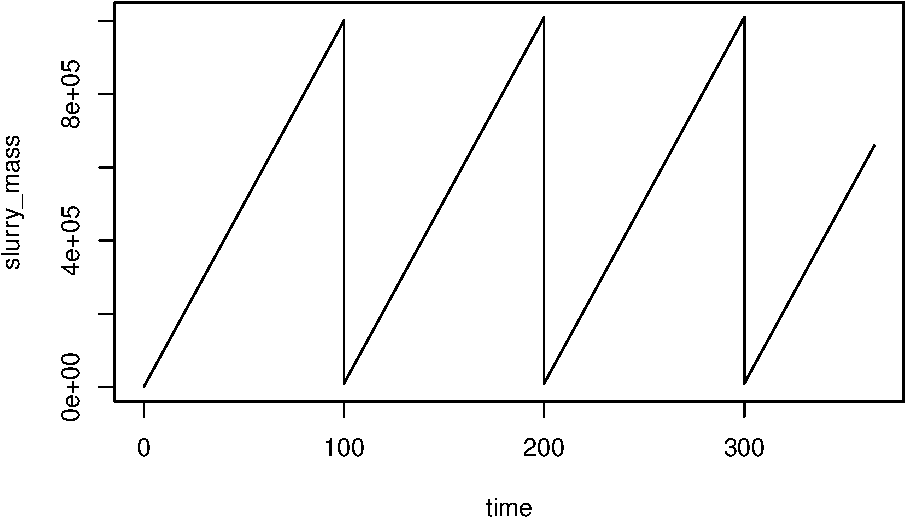
\includegraphics{simple_demo_files/figure-latex/unnamed-chunk-9-1.pdf}

\begin{Shaded}
\begin{Highlighting}[]
\FunctionTok{plot}\NormalTok{(CH4\_emis\_rate }\SpecialCharTok{\textasciitilde{}}\NormalTok{ time, }\AttributeTok{data =}\NormalTok{ out1, }\AttributeTok{type =} \StringTok{\textquotesingle{}l\textquotesingle{}}\NormalTok{)}
\end{Highlighting}
\end{Shaded}

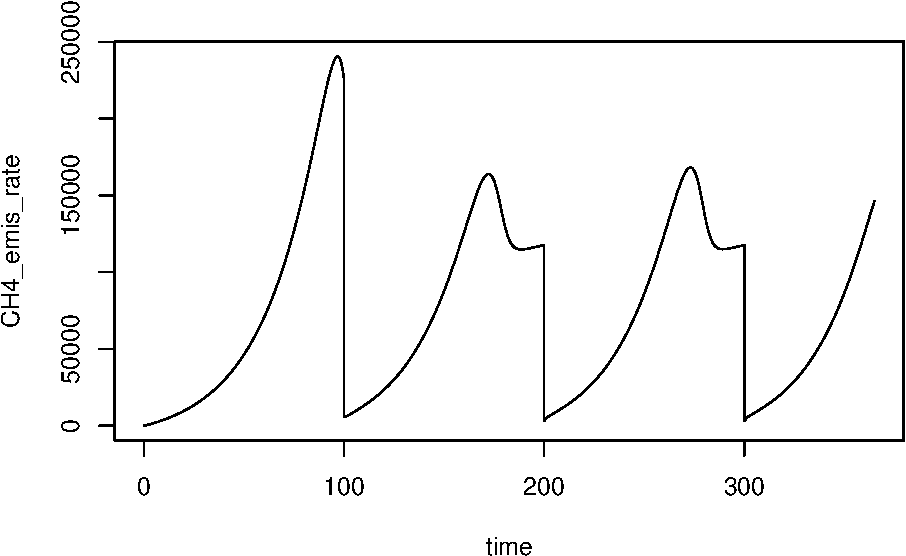
\includegraphics{simple_demo_files/figure-latex/unnamed-chunk-9-2.pdf}

\begin{Shaded}
\begin{Highlighting}[]
\FunctionTok{plot}\NormalTok{(VSd\_conc }\SpecialCharTok{\textasciitilde{}}\NormalTok{ time, }\AttributeTok{data =}\NormalTok{ out1, }\AttributeTok{type =} \StringTok{\textquotesingle{}l\textquotesingle{}}\NormalTok{)}
\end{Highlighting}
\end{Shaded}

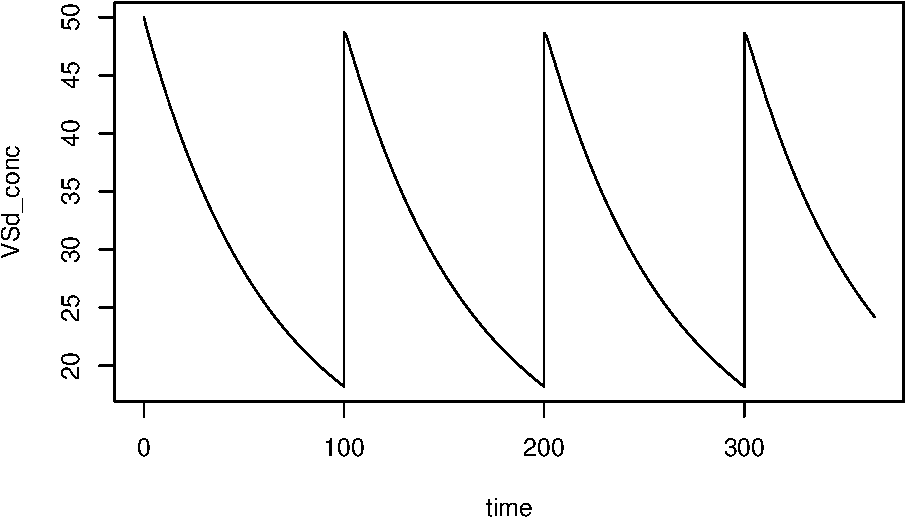
\includegraphics{simple_demo_files/figure-latex/unnamed-chunk-9-3.pdf}

\begin{Shaded}
\begin{Highlighting}[]
\FunctionTok{plot}\NormalTok{(CH3COOH\_conc }\SpecialCharTok{\textasciitilde{}}\NormalTok{ time, }\AttributeTok{data =}\NormalTok{ out1, }\AttributeTok{type =} \StringTok{\textquotesingle{}l\textquotesingle{}}\NormalTok{)}
\end{Highlighting}
\end{Shaded}

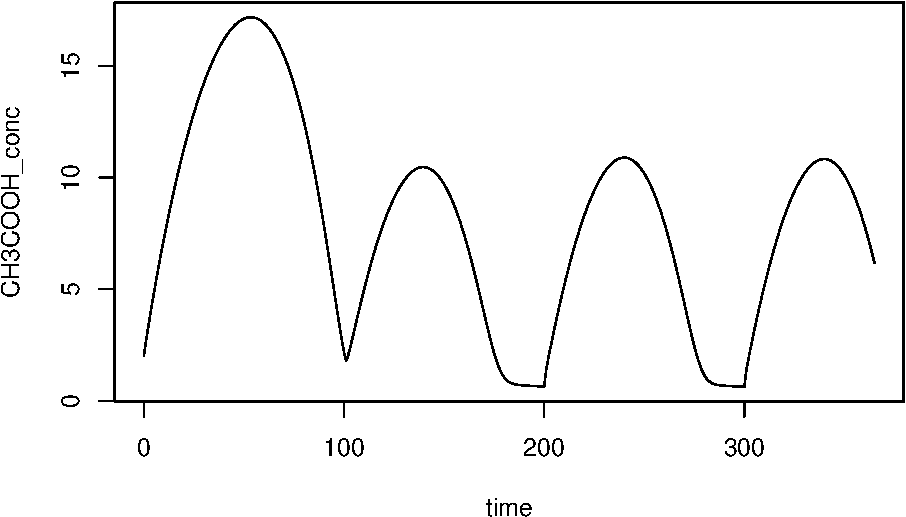
\includegraphics{simple_demo_files/figure-latex/unnamed-chunk-9-4.pdf}

And methanogens.

\begin{Shaded}
\begin{Highlighting}[]
\NormalTok{line\_colors }\OtherTok{\textless{}{-}} \FunctionTok{c}\NormalTok{(}\StringTok{\textquotesingle{}red\textquotesingle{}}\NormalTok{, }\StringTok{\textquotesingle{}blue\textquotesingle{}}\NormalTok{, }\StringTok{\textquotesingle{}purple\textquotesingle{}}\NormalTok{,}\StringTok{\textquotesingle{}orange\textquotesingle{}}\NormalTok{)}
\FunctionTok{matplot}\NormalTok{(out1}\SpecialCharTok{$}\NormalTok{time, out1[, nn }\OtherTok{\textless{}{-}} \FunctionTok{c}\NormalTok{(}\StringTok{\textquotesingle{}m0\textquotesingle{}}\NormalTok{,}\StringTok{\textquotesingle{}m1\textquotesingle{}}\NormalTok{,}\StringTok{\textquotesingle{}m2\textquotesingle{}}\NormalTok{,}\StringTok{\textquotesingle{}sr1\textquotesingle{}}\NormalTok{)]}\SpecialCharTok{/}\DecValTok{1000}\NormalTok{, }
        \AttributeTok{type =} \StringTok{\textquotesingle{}l\textquotesingle{}}\NormalTok{, }\AttributeTok{lty =} \FunctionTok{c}\NormalTok{(}\DecValTok{1}\SpecialCharTok{:}\FunctionTok{length}\NormalTok{(nn)), }\AttributeTok{col =}\NormalTok{ line\_colors, }\AttributeTok{ylab =} \StringTok{\textquotesingle{}Microbial biomass (kg)\textquotesingle{}}\NormalTok{)}
\FunctionTok{legend}\NormalTok{(}\StringTok{"topright"}\NormalTok{, }\AttributeTok{legend =}\NormalTok{ nn, }\AttributeTok{lty =} \FunctionTok{c}\NormalTok{(}\DecValTok{1}\SpecialCharTok{:}\FunctionTok{length}\NormalTok{(nn)), }\AttributeTok{col =}\NormalTok{ line\_colors, }\AttributeTok{lwd =} \DecValTok{1}\NormalTok{, }\AttributeTok{cex =} \FloatTok{0.8}\NormalTok{)}
\end{Highlighting}
\end{Shaded}

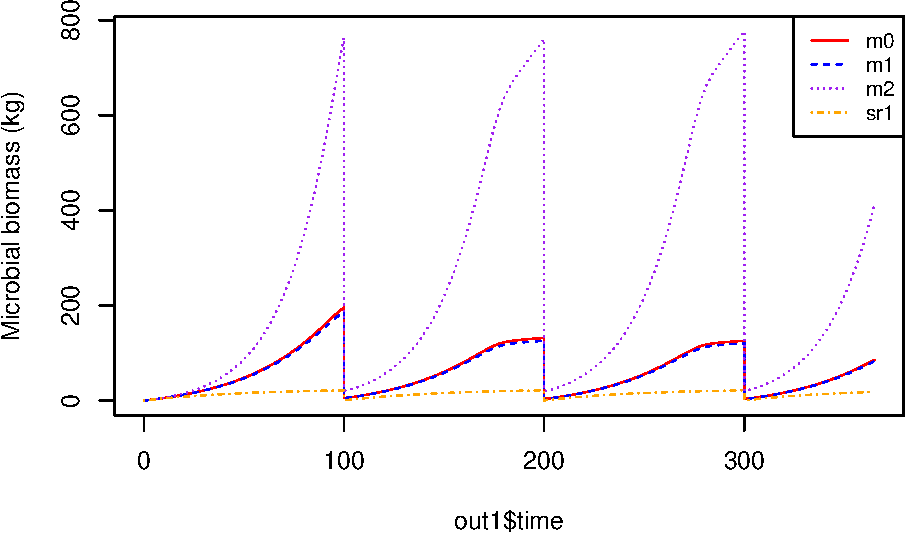
\includegraphics{simple_demo_files/figure-latex/unnamed-chunk-10-1.pdf}

\hypertarget{substrate-flexibility}{%
\section{2. Substrate flexibility}\label{substrate-flexibility}}

Particulate substrates are defined in \texttt{sub\_pars} now and there
are no specific substrates hard-wired in the code. VFA is the only
intermediate, and it is hard-wired. Here we will use three substrates.
Parameter values have no connection to reality in this example.

\begin{Shaded}
\begin{Highlighting}[]
\NormalTok{sub\_pars2 }\OtherTok{\textless{}{-}} \FunctionTok{list}\NormalTok{(}\AttributeTok{subs =} \FunctionTok{c}\NormalTok{(}\StringTok{\textquotesingle{}cellulose\textquotesingle{}}\NormalTok{, }\StringTok{\textquotesingle{}protein\textquotesingle{}}\NormalTok{, }\StringTok{\textquotesingle{}lipids\textquotesingle{}}\NormalTok{),}
                  \AttributeTok{T\_opt\_hyd =} \FunctionTok{c}\NormalTok{(}\AttributeTok{all =} \DecValTok{60}\NormalTok{),}
                  \AttributeTok{T\_min\_hyd =} \FunctionTok{c}\NormalTok{(}\AttributeTok{all =} \DecValTok{0}\NormalTok{),}
                  \AttributeTok{T\_max\_hyd =} \FunctionTok{c}\NormalTok{(}\AttributeTok{all =} \DecValTok{90}\NormalTok{),}
                  \AttributeTok{hydrol\_opt =} \FunctionTok{c}\NormalTok{(}\AttributeTok{lipids =} \FloatTok{0.1}\NormalTok{, }\AttributeTok{protein =} \FloatTok{0.01}\NormalTok{, }\AttributeTok{cellulose =} \FloatTok{0.05}\NormalTok{),}
                  \AttributeTok{sub\_fresh =} \FunctionTok{c}\NormalTok{(}\AttributeTok{lipids =} \DecValTok{3}\NormalTok{, }\AttributeTok{protein =} \DecValTok{20}\NormalTok{, }\AttributeTok{cellulose =} \DecValTok{35}\NormalTok{),}
                  \AttributeTok{sub\_init =} \FunctionTok{c}\NormalTok{(}\AttributeTok{lipids =} \DecValTok{3}\NormalTok{, }\AttributeTok{protein =} \DecValTok{20}\NormalTok{, }\AttributeTok{cellulose =} \DecValTok{35}\NormalTok{))}
\end{Highlighting}
\end{Shaded}

\begin{Shaded}
\begin{Highlighting}[]
\NormalTok{devtools}\SpecialCharTok{::}\FunctionTok{load\_all}\NormalTok{()}
\end{Highlighting}
\end{Shaded}

\begin{verbatim}
## i Loading ABM
\end{verbatim}

\begin{Shaded}
\begin{Highlighting}[]
\NormalTok{out2 }\OtherTok{\textless{}{-}} \FunctionTok{abm}\NormalTok{(}\DecValTok{365}\NormalTok{,}
            \AttributeTok{mng\_pars =}\NormalTok{ mng\_pars,}
            \AttributeTok{man\_pars =}\NormalTok{ man\_pars,}
            \AttributeTok{grp\_pars =}\NormalTok{ grp\_pars,}
            \AttributeTok{mic\_pars =}\NormalTok{ mic\_pars,}
            \AttributeTok{sub\_pars =}\NormalTok{ sub\_pars2,}
            \AttributeTok{chem\_pars =}\NormalTok{ chem\_pars)}
\end{Highlighting}
\end{Shaded}

\begin{verbatim}
## Warning in expandPars(pars = pars, elnms = pars$grps, parnms = grp_par_nms):
## Size-variable parameter problem: Missing element(s) in kss.
\end{verbatim}

\begin{Shaded}
\begin{Highlighting}[]
\FunctionTok{plot}\NormalTok{(slurry\_mass }\SpecialCharTok{\textasciitilde{}}\NormalTok{ time, }\AttributeTok{data =}\NormalTok{ out2, }\AttributeTok{type =} \StringTok{\textquotesingle{}l\textquotesingle{}}\NormalTok{)}
\FunctionTok{lines}\NormalTok{(slurry\_mass }\SpecialCharTok{\textasciitilde{}}\NormalTok{ time, }\AttributeTok{data =}\NormalTok{ out1, }\AttributeTok{col =} \StringTok{\textquotesingle{}red\textquotesingle{}}\NormalTok{)}
\end{Highlighting}
\end{Shaded}

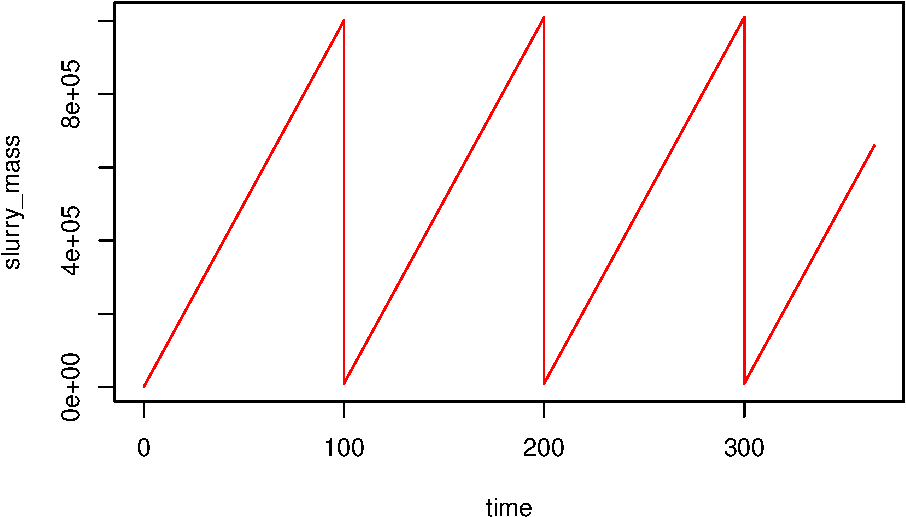
\includegraphics{simple_demo_files/figure-latex/unnamed-chunk-13-1.pdf}

\begin{Shaded}
\begin{Highlighting}[]
\FunctionTok{plot}\NormalTok{(CH4\_emis\_rate }\SpecialCharTok{\textasciitilde{}}\NormalTok{ time, }\AttributeTok{data =}\NormalTok{ out1, }\AttributeTok{type =} \StringTok{\textquotesingle{}l\textquotesingle{}}\NormalTok{)}
\FunctionTok{lines}\NormalTok{(CH4\_emis\_rate }\SpecialCharTok{\textasciitilde{}}\NormalTok{ time, }\AttributeTok{data =}\NormalTok{ out2, }\AttributeTok{col =} \StringTok{\textquotesingle{}red\textquotesingle{}}\NormalTok{)}
\end{Highlighting}
\end{Shaded}

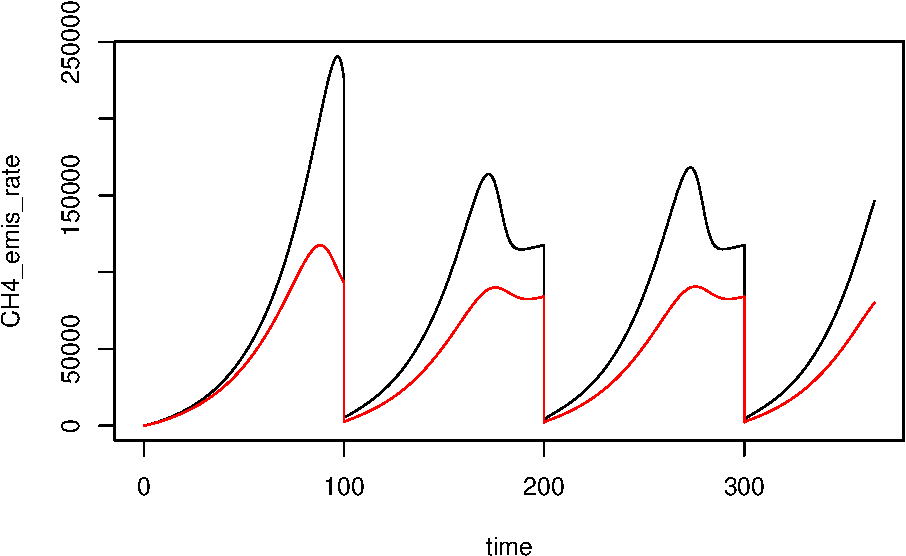
\includegraphics{simple_demo_files/figure-latex/unnamed-chunk-13-2.pdf}

\begin{Shaded}
\begin{Highlighting}[]
\FunctionTok{plot}\NormalTok{(cellulose\_conc }\SpecialCharTok{\textasciitilde{}}\NormalTok{ time, }\AttributeTok{data =}\NormalTok{ out2, }\AttributeTok{type =} \StringTok{\textquotesingle{}l\textquotesingle{}}\NormalTok{, }\AttributeTok{ylim =} \FunctionTok{c}\NormalTok{(}\DecValTok{0}\NormalTok{, }\DecValTok{35}\NormalTok{))}
\FunctionTok{lines}\NormalTok{(lipids\_conc }\SpecialCharTok{\textasciitilde{}}\NormalTok{ time, }\AttributeTok{data =}\NormalTok{ out2, }\AttributeTok{type =} \StringTok{\textquotesingle{}l\textquotesingle{}}\NormalTok{, }\AttributeTok{col =} \StringTok{\textquotesingle{}red\textquotesingle{}}\NormalTok{)}
\FunctionTok{lines}\NormalTok{(protein\_conc }\SpecialCharTok{\textasciitilde{}}\NormalTok{ time, }\AttributeTok{data =}\NormalTok{ out2, }\AttributeTok{type =} \StringTok{\textquotesingle{}l\textquotesingle{}}\NormalTok{, }\AttributeTok{col =} \StringTok{\textquotesingle{}blue\textquotesingle{}}\NormalTok{)}
\end{Highlighting}
\end{Shaded}

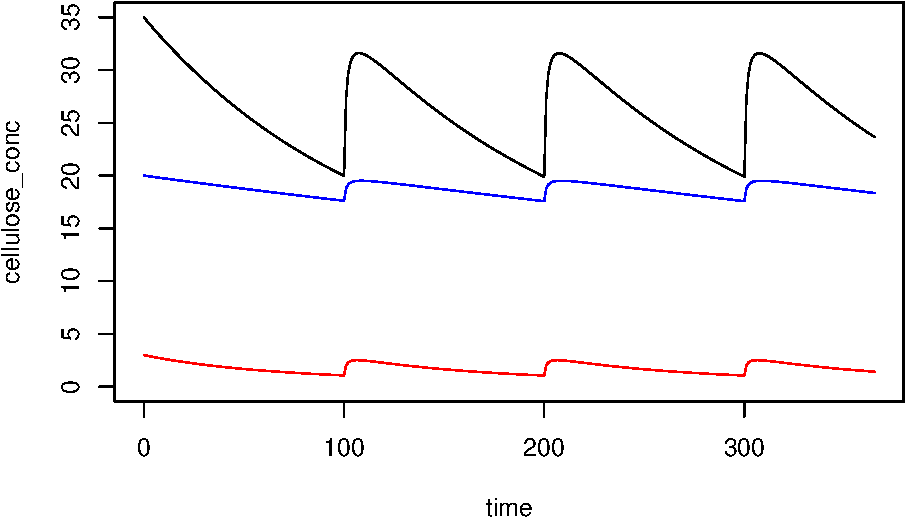
\includegraphics{simple_demo_files/figure-latex/unnamed-chunk-13-3.pdf}

\begin{Shaded}
\begin{Highlighting}[]
\FunctionTok{plot}\NormalTok{(CH3COOH\_conc }\SpecialCharTok{\textasciitilde{}}\NormalTok{ time, }\AttributeTok{data =}\NormalTok{ out1, }\AttributeTok{type =} \StringTok{\textquotesingle{}l\textquotesingle{}}\NormalTok{)}
\FunctionTok{lines}\NormalTok{(CH3COOH\_conc }\SpecialCharTok{\textasciitilde{}}\NormalTok{ time, }\AttributeTok{data =}\NormalTok{ out2, }\AttributeTok{col =} \StringTok{\textquotesingle{}red\textquotesingle{}}\NormalTok{)}
\end{Highlighting}
\end{Shaded}

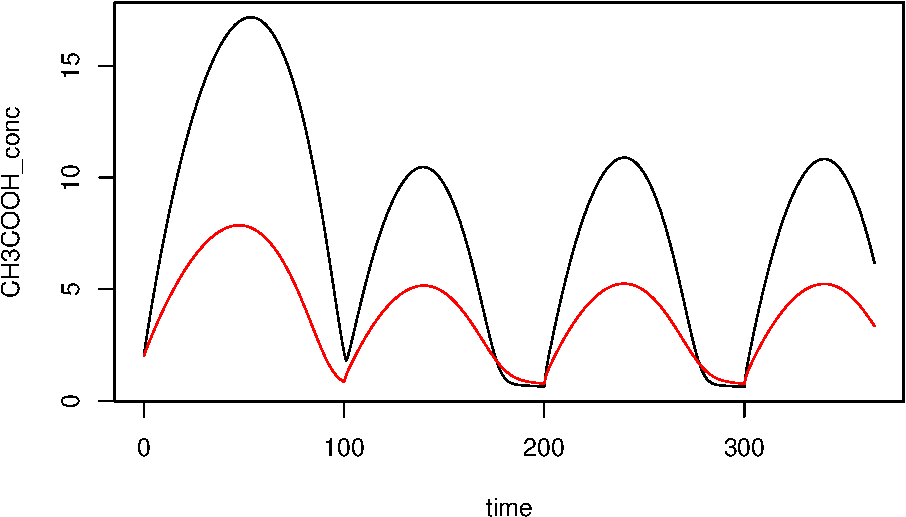
\includegraphics{simple_demo_files/figure-latex/unnamed-chunk-13-4.pdf}

This flexibility comes from an approach similar to what we used for
microbial groups.

\hypertarget{time-variable-inputs-part-1}{%
\section{3. Time-variable inputs part
1}\label{time-variable-inputs-part-1}}

The \texttt{abm()} function can handle variability over time in any
inputs now. Here slurry mass and temperature will vary.

\begin{Shaded}
\begin{Highlighting}[]
\NormalTok{var\_dat }\OtherTok{\textless{}{-}} \FunctionTok{data.frame}\NormalTok{(}\AttributeTok{time =} \FunctionTok{c}\NormalTok{(}\DecValTok{0}\NormalTok{, }\DecValTok{1}\NormalTok{, }\DecValTok{10}\NormalTok{, }\DecValTok{15}\NormalTok{, }\DecValTok{30}\NormalTok{), }
                      \AttributeTok{slurry\_mass =} \FunctionTok{c}\NormalTok{(}\DecValTok{1000}\NormalTok{, }\DecValTok{7000}\NormalTok{, }\DecValTok{2000}\NormalTok{, }\DecValTok{1500}\NormalTok{, }\DecValTok{3000}\NormalTok{),}
                      \AttributeTok{temp\_C =} \FunctionTok{c}\NormalTok{(}\DecValTok{10}\NormalTok{, }\DecValTok{15}\NormalTok{, }\DecValTok{15}\NormalTok{, }\DecValTok{20}\NormalTok{, }\DecValTok{20}\NormalTok{))}

\FunctionTok{plot}\NormalTok{(slurry\_mass }\SpecialCharTok{\textasciitilde{}}\NormalTok{ time, }\AttributeTok{data =}\NormalTok{ var\_dat, }\AttributeTok{type =} \StringTok{\textquotesingle{}o\textquotesingle{}}\NormalTok{)}
\end{Highlighting}
\end{Shaded}

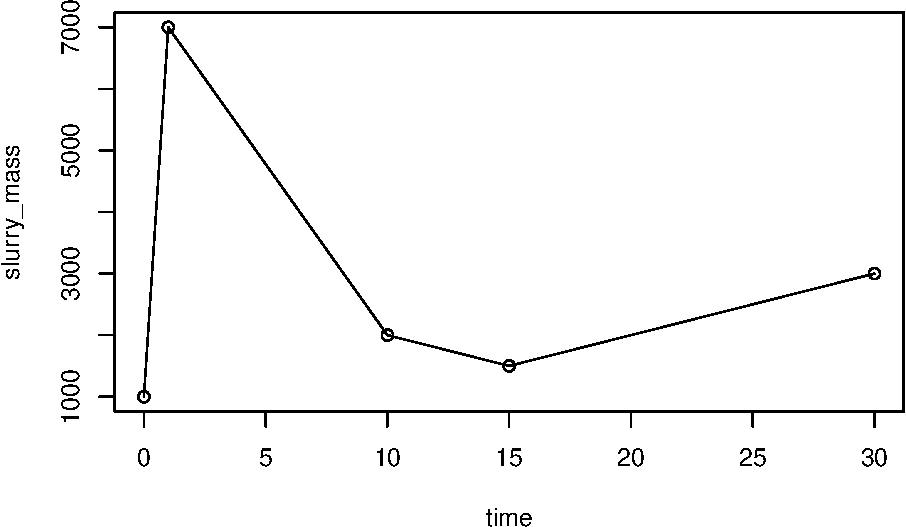
\includegraphics{simple_demo_files/figure-latex/unnamed-chunk-14-1.pdf}

\begin{Shaded}
\begin{Highlighting}[]
\FunctionTok{plot}\NormalTok{(temp\_C }\SpecialCharTok{\textasciitilde{}}\NormalTok{ time, }\AttributeTok{data =}\NormalTok{ var\_dat, }\AttributeTok{type =} \StringTok{\textquotesingle{}o\textquotesingle{}}\NormalTok{)}
\end{Highlighting}
\end{Shaded}

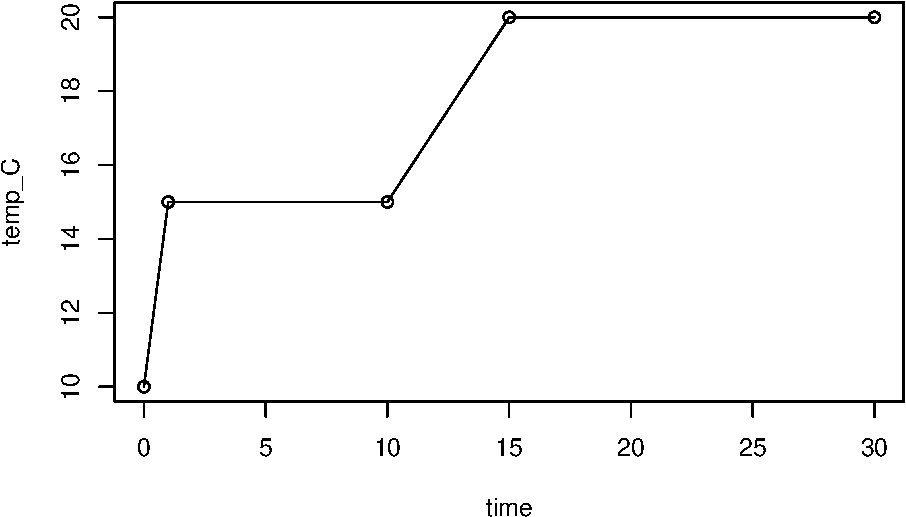
\includegraphics{simple_demo_files/figure-latex/unnamed-chunk-14-2.pdf}

This data frame goes in the \texttt{var\_pars} argument, which must be a
list, even though it might have a single element named \texttt{var}. The
\texttt{var} element is the only required one. The \texttt{var} data
frame must have a \texttt{slurry\_mass} column if it is used--it is not
possible to use an \texttt{abm\_regular()}-like approach with variable
temperature etc.

\begin{Shaded}
\begin{Highlighting}[]
\NormalTok{var\_pars }\OtherTok{\textless{}{-}} \FunctionTok{list}\NormalTok{(}\AttributeTok{var =}\NormalTok{ var\_dat)}
\end{Highlighting}
\end{Shaded}

\begin{Shaded}
\begin{Highlighting}[]
\NormalTok{out3a }\OtherTok{\textless{}{-}} \FunctionTok{abm}\NormalTok{(}\DecValTok{50}\NormalTok{,}
             \AttributeTok{mng\_pars =}\NormalTok{ mng\_pars,}
             \AttributeTok{man\_pars =}\NormalTok{ man\_pars,}
             \AttributeTok{grp\_pars =}\NormalTok{ grp\_pars,}
             \AttributeTok{mic\_pars =}\NormalTok{ mic\_pars,}
             \AttributeTok{sub\_pars =}\NormalTok{ sub\_pars,}
             \AttributeTok{chem\_pars =}\NormalTok{ chem\_pars,}
             \AttributeTok{var\_pars =}\NormalTok{ var\_pars)}
\end{Highlighting}
\end{Shaded}

\begin{verbatim}
## Warning in expandPars(pars = pars, elnms = pars$grps, parnms = grp_par_nms):
## Size-variable parameter problem: Missing element(s) in kss.
\end{verbatim}

\begin{Shaded}
\begin{Highlighting}[]
\FunctionTok{plot}\NormalTok{(slurry\_mass }\SpecialCharTok{\textasciitilde{}}\NormalTok{ time, }\AttributeTok{data =}\NormalTok{ out3a, }\AttributeTok{type =} \StringTok{\textquotesingle{}l\textquotesingle{}}\NormalTok{)}
\end{Highlighting}
\end{Shaded}

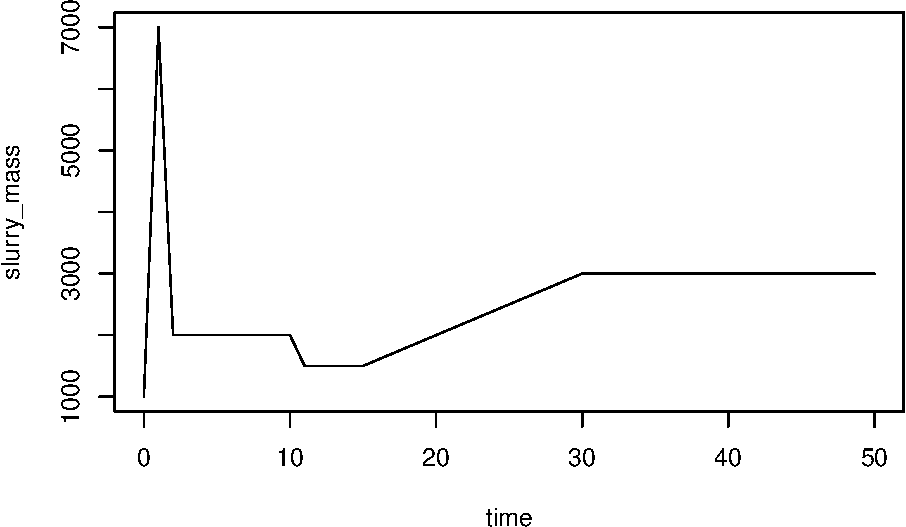
\includegraphics{simple_demo_files/figure-latex/unnamed-chunk-17-1.pdf}

The ``late'' and ``mid'' options are still available, but now through
\texttt{ctrl\_pars}. Here we can change the value through
\texttt{add\_pars}

\begin{Shaded}
\begin{Highlighting}[]
\NormalTok{out3b }\OtherTok{\textless{}{-}} \FunctionTok{abm}\NormalTok{(}\DecValTok{50}\NormalTok{,}
             \AttributeTok{mng\_pars =}\NormalTok{ mng\_pars,}
             \AttributeTok{man\_pars =}\NormalTok{ man\_pars,}
             \AttributeTok{grp\_pars =}\NormalTok{ grp\_pars,}
             \AttributeTok{mic\_pars =}\NormalTok{ mic\_pars,}
             \AttributeTok{sub\_pars =}\NormalTok{ sub\_pars,}
             \AttributeTok{chem\_pars =}\NormalTok{ chem\_pars,}
             \AttributeTok{var\_pars =}\NormalTok{ var\_pars,}
             \AttributeTok{add\_pars =} \FunctionTok{list}\NormalTok{(}\AttributeTok{approx\_method =} \StringTok{\textquotesingle{}late\textquotesingle{}}\NormalTok{))}
\end{Highlighting}
\end{Shaded}

\begin{verbatim}
## Warning in expandPars(pars = pars, elnms = pars$grps, parnms = grp_par_nms):
## Size-variable parameter problem: Missing element(s) in kss.
\end{verbatim}

\begin{Shaded}
\begin{Highlighting}[]
\NormalTok{out3c }\OtherTok{\textless{}{-}} \FunctionTok{abm}\NormalTok{(}\DecValTok{50}\NormalTok{,}
             \AttributeTok{mng\_pars =}\NormalTok{ mng\_pars,}
             \AttributeTok{man\_pars =}\NormalTok{ man\_pars,}
             \AttributeTok{grp\_pars =}\NormalTok{ grp\_pars,}
             \AttributeTok{mic\_pars =}\NormalTok{ mic\_pars,}
             \AttributeTok{sub\_pars =}\NormalTok{ sub\_pars,}
             \AttributeTok{chem\_pars =}\NormalTok{ chem\_pars,}
             \AttributeTok{var\_pars =}\NormalTok{ var\_pars,}
             \AttributeTok{add\_pars =} \FunctionTok{list}\NormalTok{(}\AttributeTok{approx\_method =} \StringTok{\textquotesingle{}mid\textquotesingle{}}\NormalTok{))}
\end{Highlighting}
\end{Shaded}

\begin{verbatim}
## Warning in expandPars(pars = pars, elnms = pars$grps, parnms = grp_par_nms):
## Size-variable parameter problem: Missing element(s) in kss.
\end{verbatim}

\begin{Shaded}
\begin{Highlighting}[]
\FunctionTok{plot}\NormalTok{(slurry\_mass }\SpecialCharTok{\textasciitilde{}}\NormalTok{ time, }\AttributeTok{data =}\NormalTok{ out3a, }\AttributeTok{type =} \StringTok{\textquotesingle{}l\textquotesingle{}}\NormalTok{)}
\FunctionTok{lines}\NormalTok{(slurry\_mass }\SpecialCharTok{\textasciitilde{}}\NormalTok{ time, }\AttributeTok{data =}\NormalTok{ out3b, }\AttributeTok{col =} \StringTok{\textquotesingle{}red\textquotesingle{}}\NormalTok{)}
\FunctionTok{lines}\NormalTok{(slurry\_mass }\SpecialCharTok{\textasciitilde{}}\NormalTok{ time, }\AttributeTok{data =}\NormalTok{ out3c, }\AttributeTok{col =} \StringTok{\textquotesingle{}blue\textquotesingle{}}\NormalTok{)}
\end{Highlighting}
\end{Shaded}

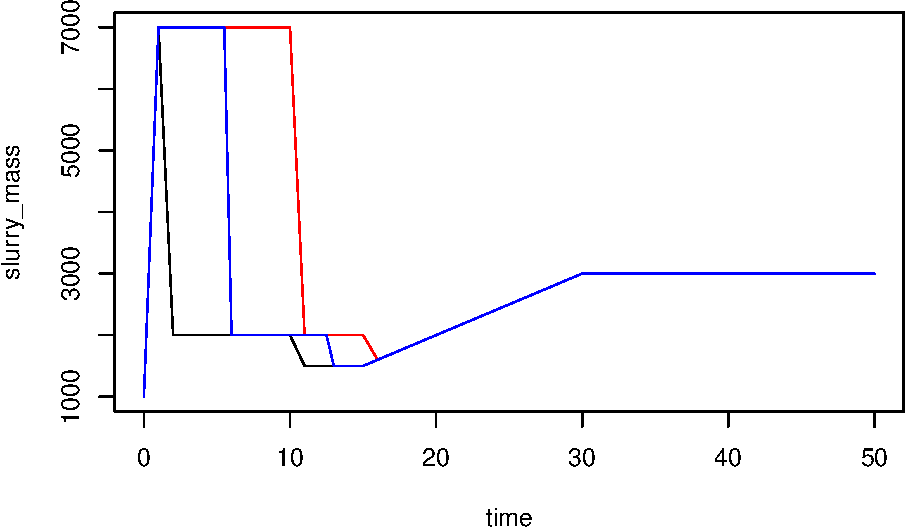
\includegraphics{simple_demo_files/figure-latex/unnamed-chunk-20-1.pdf}

\begin{Shaded}
\begin{Highlighting}[]
\FunctionTok{plot}\NormalTok{(CH4\_emis\_cum }\SpecialCharTok{\textasciitilde{}}\NormalTok{ time, }\AttributeTok{data =}\NormalTok{ out3a, }\AttributeTok{type =} \StringTok{\textquotesingle{}l\textquotesingle{}}\NormalTok{)}
\FunctionTok{lines}\NormalTok{(CH4\_emis\_cum }\SpecialCharTok{\textasciitilde{}}\NormalTok{ time, }\AttributeTok{data =}\NormalTok{ out3b, }\AttributeTok{col =} \StringTok{\textquotesingle{}red\textquotesingle{}}\NormalTok{)}
\FunctionTok{lines}\NormalTok{(CH4\_emis\_cum }\SpecialCharTok{\textasciitilde{}}\NormalTok{ time, }\AttributeTok{data =}\NormalTok{ out3c, }\AttributeTok{col =} \StringTok{\textquotesingle{}blue\textquotesingle{}}\NormalTok{)}
\end{Highlighting}
\end{Shaded}

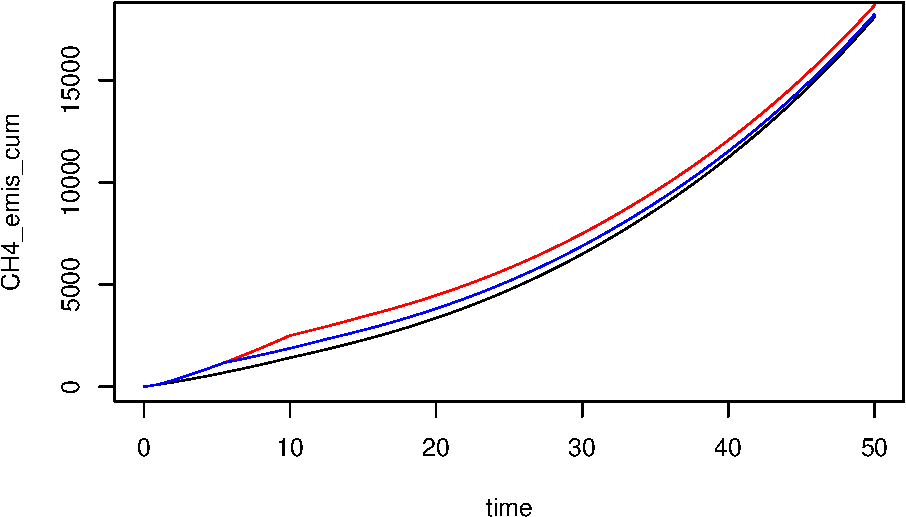
\includegraphics{simple_demo_files/figure-latex/unnamed-chunk-21-1.pdf}

\hypertarget{time-variable-inputs-part-2}{%
\section{4. Time-variable inputs part
2}\label{time-variable-inputs-part-2}}

Here we'll vary fresh substrate concentrations over time.

First the data frame with slurry mass.

\begin{Shaded}
\begin{Highlighting}[]
\NormalTok{var\_dat }\OtherTok{\textless{}{-}} \FunctionTok{data.frame}\NormalTok{(}\AttributeTok{time =} \FunctionTok{c}\NormalTok{(}\DecValTok{0}\NormalTok{, }\DecValTok{1}\NormalTok{, }\DecValTok{10}\NormalTok{, }\DecValTok{15}\NormalTok{, }\DecValTok{30}\NormalTok{, }\DecValTok{50}\NormalTok{), }
                      \AttributeTok{slurry\_mass =} \FunctionTok{c}\NormalTok{(}\DecValTok{1000}\NormalTok{, }\DecValTok{7000}\NormalTok{, }\DecValTok{2000}\NormalTok{, }\DecValTok{5000}\NormalTok{, }\DecValTok{3000}\NormalTok{, }\DecValTok{10000}\NormalTok{))}
\NormalTok{var\_dat}
\end{Highlighting}
\end{Shaded}

\begin{verbatim}
##   time slurry_mass
## 1    0        1000
## 2    1        7000
## 3   10        2000
## 4   15        5000
## 5   30        3000
## 6   50       10000
\end{verbatim}

Then add \texttt{sub\_fresh} values. Each row needs a list containing a
named vector. This is somewhat unusual data frame usage, and there is a
user-friendly alternative based on additional data frames in the
\texttt{var} argument (see next section). But I've kept this demo.

\begin{Shaded}
\begin{Highlighting}[]
\NormalTok{var\_dat}
\end{Highlighting}
\end{Shaded}

\begin{verbatim}
##   time slurry_mass
## 1    0        1000
## 2    1        7000
## 3   10        2000
## 4   15        5000
## 5   30        3000
## 6   50       10000
\end{verbatim}

\begin{Shaded}
\begin{Highlighting}[]
\NormalTok{var\_dat}\SpecialCharTok{$}\NormalTok{sub\_fresh }\OtherTok{\textless{}{-}} \FunctionTok{rep}\NormalTok{(}\FunctionTok{list}\NormalTok{(}\FunctionTok{c}\NormalTok{(}\AttributeTok{VSd =} \DecValTok{50}\NormalTok{)), }\FunctionTok{nrow}\NormalTok{(var\_dat))}
\NormalTok{var\_dat}\SpecialCharTok{$}\NormalTok{sub\_fresh[}\DecValTok{3}\NormalTok{] }\OtherTok{\textless{}{-}} \FunctionTok{list}\NormalTok{(}\FunctionTok{c}\NormalTok{(}\AttributeTok{VSd =} \DecValTok{100}\NormalTok{))}
\NormalTok{var\_dat}\SpecialCharTok{$}\NormalTok{sub\_fresh[}\DecValTok{4}\NormalTok{] }\OtherTok{\textless{}{-}} \FunctionTok{list}\NormalTok{(}\FunctionTok{c}\NormalTok{(}\AttributeTok{VSd =} \DecValTok{10}\NormalTok{))}
\NormalTok{var\_dat}\SpecialCharTok{$}\NormalTok{sub\_fresh[}\DecValTok{5}\NormalTok{] }\OtherTok{\textless{}{-}} \FunctionTok{list}\NormalTok{(}\FunctionTok{c}\NormalTok{(}\AttributeTok{VSd =} \DecValTok{0}\NormalTok{))}
\NormalTok{var\_dat}\SpecialCharTok{$}\NormalTok{sub\_fresh[}\DecValTok{6}\NormalTok{] }\OtherTok{\textless{}{-}} \FunctionTok{list}\NormalTok{(}\FunctionTok{c}\NormalTok{(}\AttributeTok{VSd =} \DecValTok{200}\NormalTok{))}
\NormalTok{var\_dat}
\end{Highlighting}
\end{Shaded}

\begin{verbatim}
##   time slurry_mass sub_fresh
## 1    0        1000        50
## 2    1        7000        50
## 3   10        2000       100
## 4   15        5000        10
## 5   30        3000         0
## 6   50       10000       200
\end{verbatim}

\begin{Shaded}
\begin{Highlighting}[]
\NormalTok{var\_dat[}\DecValTok{1}\NormalTok{, }\DecValTok{3}\NormalTok{]}
\end{Highlighting}
\end{Shaded}

\begin{verbatim}
## [[1]]
## VSd 
##  50
\end{verbatim}

\begin{Shaded}
\begin{Highlighting}[]
\NormalTok{var\_dat[}\DecValTok{5}\NormalTok{, }\DecValTok{3}\NormalTok{]}
\end{Highlighting}
\end{Shaded}

\begin{verbatim}
## [[1]]
## VSd 
##   0
\end{verbatim}

\begin{Shaded}
\begin{Highlighting}[]
\NormalTok{devtools}\SpecialCharTok{::}\FunctionTok{load\_all}\NormalTok{()}
\end{Highlighting}
\end{Shaded}

\begin{verbatim}
## i Loading ABM
\end{verbatim}

\begin{Shaded}
\begin{Highlighting}[]
\NormalTok{out4a }\OtherTok{\textless{}{-}} \FunctionTok{abm}\NormalTok{(}\DecValTok{100}\NormalTok{,}
             \AttributeTok{mng\_pars =}\NormalTok{ mng\_pars,}
             \AttributeTok{man\_pars =}\NormalTok{ man\_pars,}
             \AttributeTok{grp\_pars =}\NormalTok{ grp\_pars,}
             \AttributeTok{mic\_pars =}\NormalTok{ mic\_pars,}
             \AttributeTok{sub\_pars =}\NormalTok{ sub\_pars,}
             \AttributeTok{chem\_pars =}\NormalTok{ chem\_pars,}
             \AttributeTok{var\_pars =}\NormalTok{ var\_pars)}
\end{Highlighting}
\end{Shaded}

\begin{verbatim}
## Warning in expandPars(pars = pars, elnms = pars$grps, parnms = grp_par_nms):
## Size-variable parameter problem: Missing element(s) in kss.
\end{verbatim}

\begin{Shaded}
\begin{Highlighting}[]
\FunctionTok{plot}\NormalTok{(slurry\_mass }\SpecialCharTok{\textasciitilde{}}\NormalTok{ time, }\AttributeTok{data =}\NormalTok{ out4a, }\AttributeTok{type =} \StringTok{\textquotesingle{}l\textquotesingle{}}\NormalTok{)}
\end{Highlighting}
\end{Shaded}

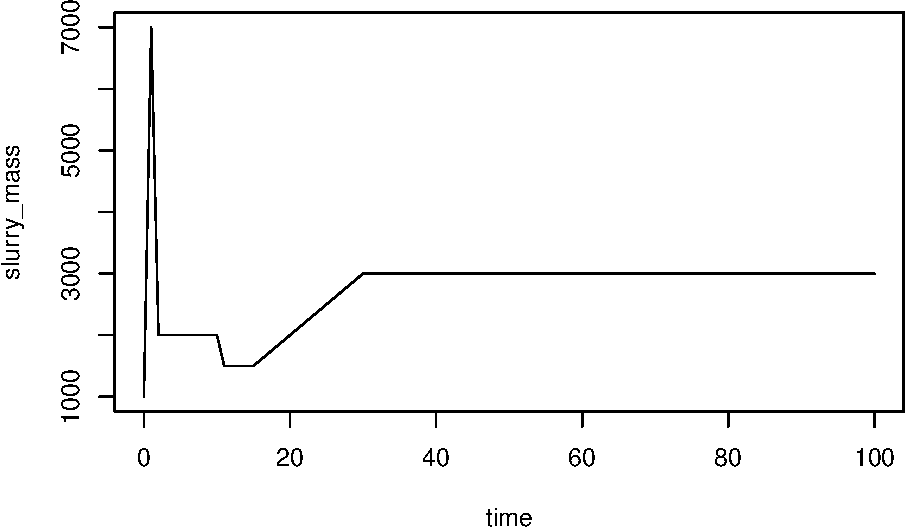
\includegraphics{simple_demo_files/figure-latex/unnamed-chunk-25-1.pdf}

\begin{Shaded}
\begin{Highlighting}[]
\FunctionTok{plot}\NormalTok{(CH4\_emis\_rate }\SpecialCharTok{\textasciitilde{}}\NormalTok{ time, }\AttributeTok{data =}\NormalTok{ out4a, }\AttributeTok{type =} \StringTok{\textquotesingle{}l\textquotesingle{}}\NormalTok{)}
\end{Highlighting}
\end{Shaded}

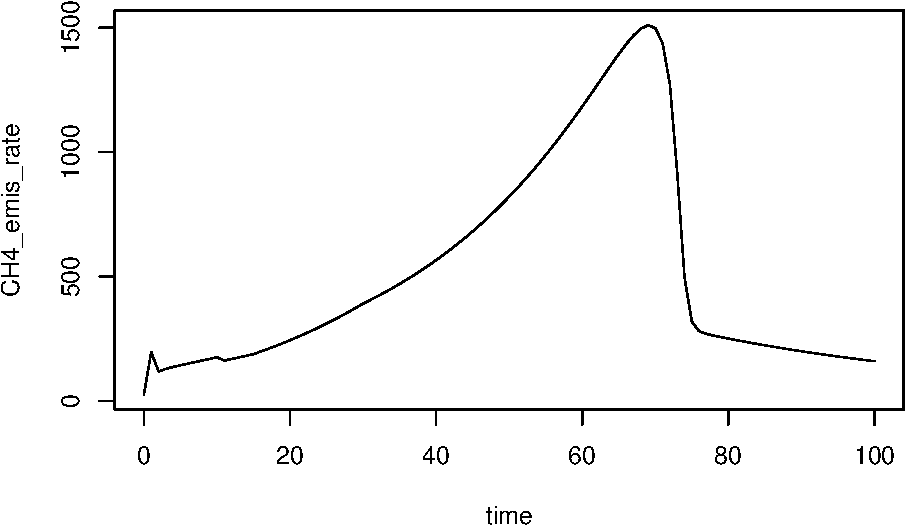
\includegraphics{simple_demo_files/figure-latex/unnamed-chunk-25-2.pdf}

\begin{Shaded}
\begin{Highlighting}[]
\FunctionTok{plot}\NormalTok{(var\_dat}\SpecialCharTok{$}\NormalTok{time, }\FunctionTok{as.vector}\NormalTok{(}\FunctionTok{lapply}\NormalTok{(var\_dat}\SpecialCharTok{$}\NormalTok{sub\_fresh, }\StringTok{\textasciigrave{}}\AttributeTok{[[}\StringTok{\textasciigrave{}}\NormalTok{, }\DecValTok{1}\NormalTok{)), }\AttributeTok{type =} \StringTok{\textquotesingle{}p\textquotesingle{}}\NormalTok{, }\AttributeTok{col =} \StringTok{\textquotesingle{}red\textquotesingle{}}\NormalTok{)}
\FunctionTok{lines}\NormalTok{(VSd\_conc }\SpecialCharTok{\textasciitilde{}}\NormalTok{ time, }\AttributeTok{data =}\NormalTok{ out4a, }\AttributeTok{type =} \StringTok{\textquotesingle{}p\textquotesingle{}}\NormalTok{)}
\end{Highlighting}
\end{Shaded}

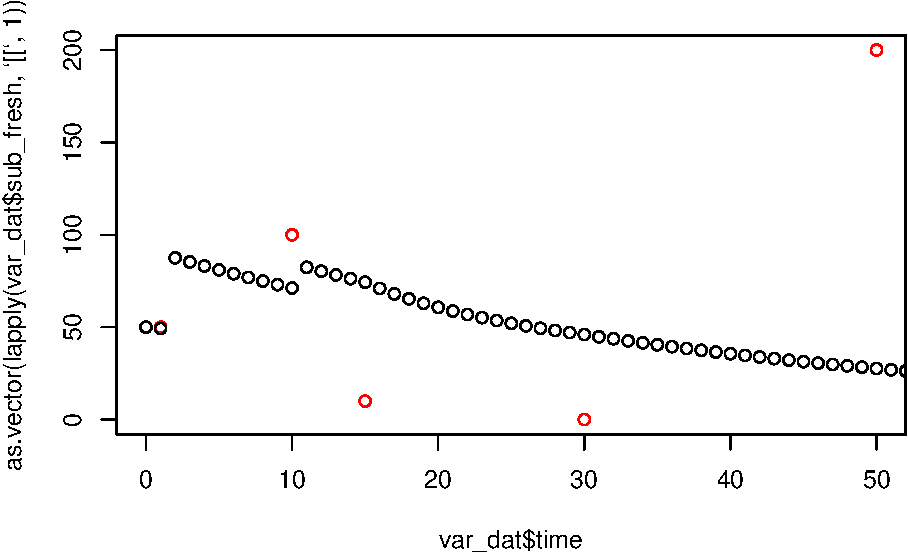
\includegraphics{simple_demo_files/figure-latex/unnamed-chunk-25-3.pdf}

\begin{Shaded}
\begin{Highlighting}[]
\FunctionTok{plot}\NormalTok{(CH3COOH\_conc }\SpecialCharTok{\textasciitilde{}}\NormalTok{ time, }\AttributeTok{data =}\NormalTok{ out4a, }\AttributeTok{type =} \StringTok{\textquotesingle{}l\textquotesingle{}}\NormalTok{)}
\end{Highlighting}
\end{Shaded}

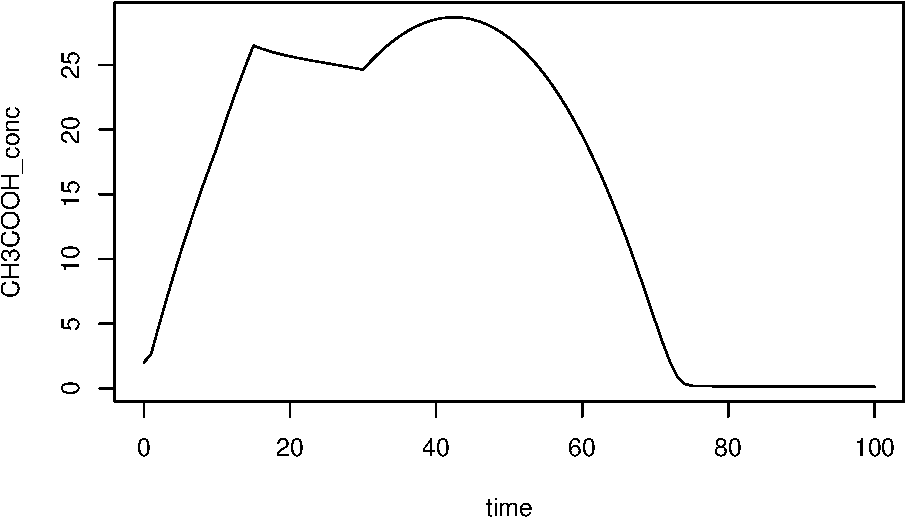
\includegraphics{simple_demo_files/figure-latex/unnamed-chunk-25-4.pdf}

Let's vary some microbial parameters as well. And pH.

\begin{Shaded}
\begin{Highlighting}[]
\NormalTok{var\_dat }\OtherTok{\textless{}{-}} \FunctionTok{data.frame}\NormalTok{(}\AttributeTok{time =} \FunctionTok{c}\NormalTok{(}\DecValTok{0}\NormalTok{, }\DecValTok{1}\NormalTok{, }\DecValTok{10}\NormalTok{, }\DecValTok{15}\NormalTok{, }\DecValTok{30}\NormalTok{, }\DecValTok{50}\NormalTok{), }
                      \AttributeTok{slurry\_mass =} \FunctionTok{c}\NormalTok{(}\DecValTok{1000}\NormalTok{, }\DecValTok{7000}\NormalTok{, }\DecValTok{2000}\NormalTok{, }\DecValTok{5000}\NormalTok{, }\DecValTok{3000}\NormalTok{, }\DecValTok{10000}\NormalTok{),}
                      \AttributeTok{pH =} \DecValTok{7} \SpecialCharTok{{-}} \DecValTok{0}\SpecialCharTok{:}\DecValTok{5}\SpecialCharTok{/}\DecValTok{10}\NormalTok{)}
\NormalTok{var\_dat}
\end{Highlighting}
\end{Shaded}

\begin{verbatim}
##   time slurry_mass  pH
## 1    0        1000 7.0
## 2    1        7000 6.9
## 3   10        2000 6.8
## 4   15        5000 6.7
## 5   30        3000 6.6
## 6   50       10000 6.5
\end{verbatim}

VSd.

\begin{Shaded}
\begin{Highlighting}[]
\NormalTok{var\_dat}\SpecialCharTok{$}\NormalTok{sub\_fresh }\OtherTok{\textless{}{-}} \FunctionTok{rep}\NormalTok{(}\FunctionTok{list}\NormalTok{(}\FunctionTok{c}\NormalTok{(}\AttributeTok{VSd =} \DecValTok{50}\NormalTok{)), }\FunctionTok{nrow}\NormalTok{(var\_dat))}
\NormalTok{var\_dat}\SpecialCharTok{$}\NormalTok{sub\_fresh[}\DecValTok{3}\NormalTok{] }\OtherTok{\textless{}{-}} \FunctionTok{list}\NormalTok{(}\FunctionTok{c}\NormalTok{(}\AttributeTok{VSd =} \DecValTok{100}\NormalTok{))}
\end{Highlighting}
\end{Shaded}

Some microbial parameters for a shift in temperature optima,
``adaptation'' for example.

\begin{Shaded}
\begin{Highlighting}[]
\ControlFlowTok{for}\NormalTok{ (i }\ControlFlowTok{in} \DecValTok{1}\SpecialCharTok{:}\FunctionTok{nrow}\NormalTok{(var\_dat)) \{}
\NormalTok{  var\_dat}\SpecialCharTok{$}\NormalTok{T\_opt[i] }\OtherTok{\textless{}{-}} \FunctionTok{list}\NormalTok{(grp\_pars}\SpecialCharTok{$}\NormalTok{T\_opt }\SpecialCharTok{+} \DecValTok{2} \SpecialCharTok{*}\NormalTok{ i)}
\NormalTok{\}}
\NormalTok{var\_dat}
\end{Highlighting}
\end{Shaded}

\begin{verbatim}
##   time slurry_mass  pH sub_fresh          T_opt
## 1    0        1000 7.0        50 20, 20, 30, 46
## 2    1        7000 6.9        50 22, 22, 32, 48
## 3   10        2000 6.8       100 24, 24, 34, 50
## 4   15        5000 6.7        50 26, 26, 36, 52
## 5   30        3000 6.6        50 28, 28, 38, 54
## 6   50       10000 6.5        50 30, 30, 40, 56
\end{verbatim}

\begin{Shaded}
\begin{Highlighting}[]
\NormalTok{out4b }\OtherTok{\textless{}{-}} \FunctionTok{abm}\NormalTok{(}\DecValTok{100}\NormalTok{,}
             \AttributeTok{mng\_pars =}\NormalTok{ mng\_pars,}
             \AttributeTok{man\_pars =}\NormalTok{ man\_pars,}
             \AttributeTok{grp\_pars =}\NormalTok{ grp\_pars,}
             \AttributeTok{mic\_pars =}\NormalTok{ mic\_pars,}
             \AttributeTok{sub\_pars =}\NormalTok{ sub\_pars,}
             \AttributeTok{chem\_pars =}\NormalTok{ chem\_pars,}
             \AttributeTok{var\_pars =}\NormalTok{ var\_pars)}
\end{Highlighting}
\end{Shaded}

\begin{verbatim}
## Warning in expandPars(pars = pars, elnms = pars$grps, parnms = grp_par_nms):
## Size-variable parameter problem: Missing element(s) in kss.
\end{verbatim}

\begin{Shaded}
\begin{Highlighting}[]
\FunctionTok{plot}\NormalTok{(slurry\_mass }\SpecialCharTok{\textasciitilde{}}\NormalTok{ time, }\AttributeTok{data =}\NormalTok{ out4b, }\AttributeTok{type =} \StringTok{\textquotesingle{}l\textquotesingle{}}\NormalTok{)}
\end{Highlighting}
\end{Shaded}

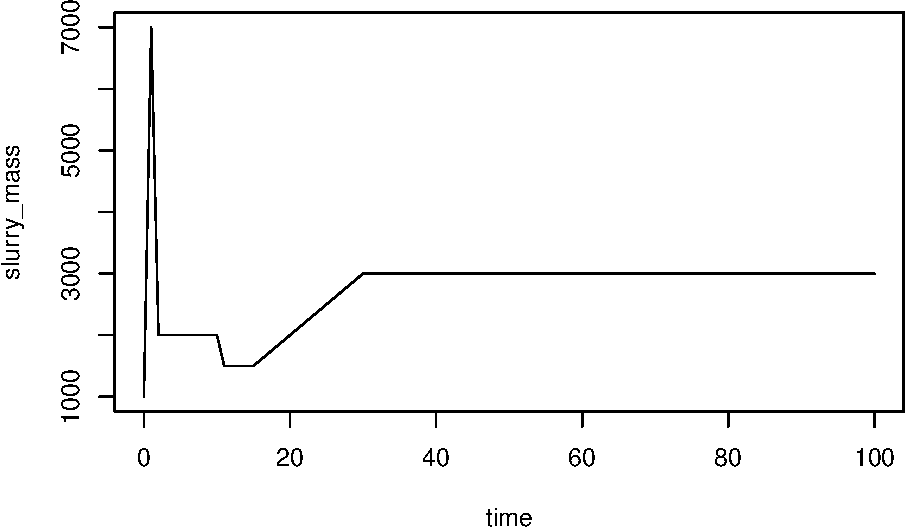
\includegraphics{simple_demo_files/figure-latex/unnamed-chunk-30-1.pdf}

\begin{Shaded}
\begin{Highlighting}[]
\FunctionTok{plot}\NormalTok{(CH4\_emis\_rate }\SpecialCharTok{\textasciitilde{}}\NormalTok{ time, }\AttributeTok{data =}\NormalTok{ out4b, }\AttributeTok{type =} \StringTok{\textquotesingle{}l\textquotesingle{}}\NormalTok{)}
\end{Highlighting}
\end{Shaded}

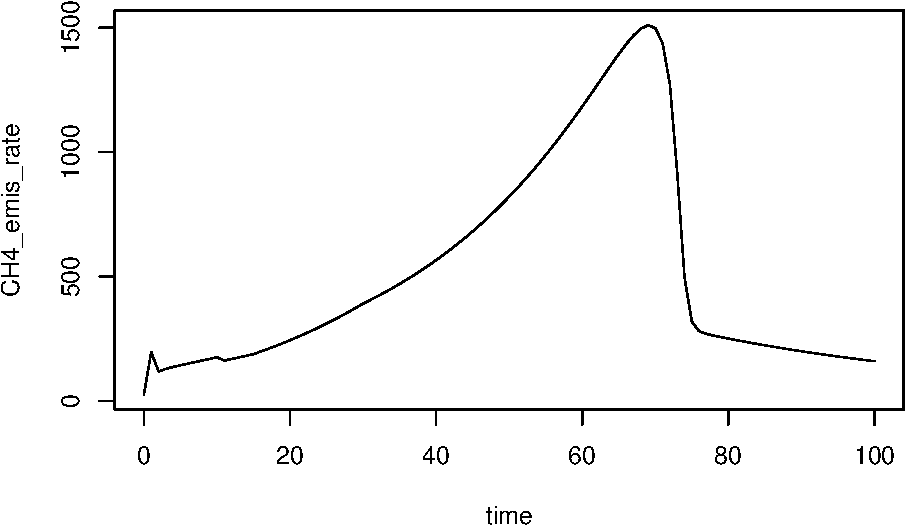
\includegraphics{simple_demo_files/figure-latex/unnamed-chunk-30-2.pdf}

\begin{Shaded}
\begin{Highlighting}[]
\FunctionTok{plot}\NormalTok{(VSd\_conc }\SpecialCharTok{\textasciitilde{}}\NormalTok{ time, }\AttributeTok{data =}\NormalTok{ out4b, }\AttributeTok{type =} \StringTok{\textquotesingle{}l\textquotesingle{}}\NormalTok{)}
\end{Highlighting}
\end{Shaded}

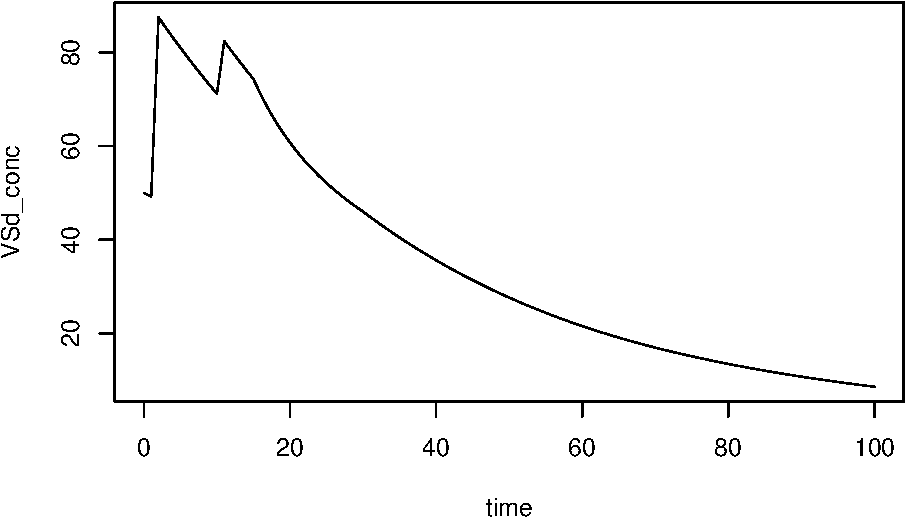
\includegraphics{simple_demo_files/figure-latex/unnamed-chunk-30-3.pdf}

\begin{Shaded}
\begin{Highlighting}[]
\FunctionTok{plot}\NormalTok{(CH3COOH\_conc }\SpecialCharTok{\textasciitilde{}}\NormalTok{ time, }\AttributeTok{data =}\NormalTok{ out4b, }\AttributeTok{type =} \StringTok{\textquotesingle{}l\textquotesingle{}}\NormalTok{)}
\end{Highlighting}
\end{Shaded}

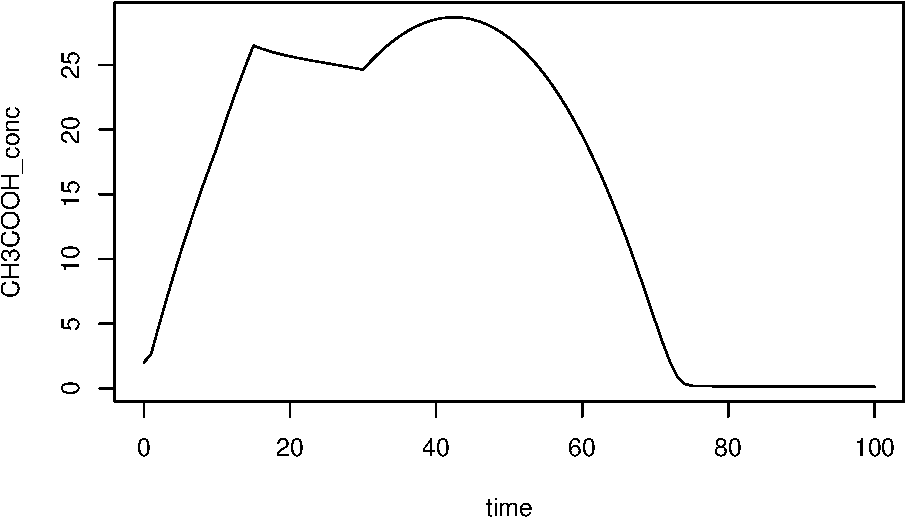
\includegraphics{simple_demo_files/figure-latex/unnamed-chunk-30-4.pdf}

\hypertarget{time-variable-inputs-part-3}{%
\section{5. Time-variable inputs part
3}\label{time-variable-inputs-part-3}}

The list-in-data frame approach is clunky. Here is an alternative.

\begin{Shaded}
\begin{Highlighting}[]
\NormalTok{var\_dat }\OtherTok{\textless{}{-}} \FunctionTok{data.frame}\NormalTok{(}\AttributeTok{time =} \FunctionTok{c}\NormalTok{(}\DecValTok{0}\NormalTok{, }\DecValTok{1}\NormalTok{, }\DecValTok{10}\NormalTok{, }\DecValTok{15}\NormalTok{, }\DecValTok{30}\NormalTok{, }\DecValTok{50}\NormalTok{), }
                      \AttributeTok{slurry\_mass =} \FunctionTok{c}\NormalTok{(}\DecValTok{1000}\NormalTok{, }\DecValTok{7000}\NormalTok{, }\DecValTok{2000}\NormalTok{, }\DecValTok{5000}\NormalTok{, }\DecValTok{3000}\NormalTok{, }\DecValTok{10000}\NormalTok{))}
\NormalTok{var\_dat}
\end{Highlighting}
\end{Shaded}

\begin{verbatim}
##   time slurry_mass
## 1    0        1000
## 2    1        7000
## 3   10        2000
## 4   15        5000
## 5   30        3000
## 6   50       10000
\end{verbatim}

Make a separate data frame for each other argument (any name, but note
column names!).

\begin{Shaded}
\begin{Highlighting}[]
\NormalTok{sub\_fresh\_dat }\OtherTok{=} \FunctionTok{data.frame}\NormalTok{(}\AttributeTok{time =} \FunctionTok{c}\NormalTok{(}\DecValTok{0}\NormalTok{, }\DecValTok{1}\NormalTok{, }\DecValTok{10}\NormalTok{, }\DecValTok{15}\NormalTok{, }\DecValTok{30}\NormalTok{, }\DecValTok{50}\NormalTok{), }
                       \AttributeTok{VSd =} \FunctionTok{c}\NormalTok{(}\DecValTok{50}\NormalTok{, }\DecValTok{100}\NormalTok{, }\DecValTok{0}\NormalTok{, }\DecValTok{0}\NormalTok{, }\DecValTok{200}\NormalTok{, }\DecValTok{50}\NormalTok{))}
\end{Highlighting}
\end{Shaded}

\begin{Shaded}
\begin{Highlighting}[]
\NormalTok{T\_opt\_dat }\OtherTok{=} \FunctionTok{data.frame}\NormalTok{(}\AttributeTok{time =} \FunctionTok{c}\NormalTok{(}\DecValTok{0}\NormalTok{, }\DecValTok{1}\NormalTok{, }\DecValTok{10}\NormalTok{, }\DecValTok{15}\NormalTok{, }\DecValTok{30}\NormalTok{, }\DecValTok{50}\NormalTok{), }
                       \AttributeTok{m1 =} \DecValTok{20} \SpecialCharTok{+} \DecValTok{0}\SpecialCharTok{:}\DecValTok{5} \SpecialCharTok{*} \DecValTok{2}\NormalTok{,}
                       \AttributeTok{m2 =} \DecValTok{20} \SpecialCharTok{+} \DecValTok{0}\SpecialCharTok{:}\DecValTok{5} \SpecialCharTok{*} \DecValTok{2}\NormalTok{,}
                       \AttributeTok{m3 =} \DecValTok{30} \SpecialCharTok{+} \DecValTok{0}\SpecialCharTok{:}\DecValTok{5} \SpecialCharTok{*} \DecValTok{2}\NormalTok{,}
                       \AttributeTok{sr1 =} \DecValTok{46} \SpecialCharTok{+} \DecValTok{0}\SpecialCharTok{:}\DecValTok{5} \SpecialCharTok{*} \DecValTok{2}\NormalTok{)}
\end{Highlighting}
\end{Shaded}

and combine them in a list, using the parameter element names for
element names (e.g., \texttt{sub\_fresh} is the name of an element in
\texttt{sub\_pars}).

\begin{Shaded}
\begin{Highlighting}[]
\NormalTok{var\_pars }\OtherTok{\textless{}{-}} \FunctionTok{list}\NormalTok{(}\AttributeTok{var =}\NormalTok{ var\_dat, }\AttributeTok{sub\_fresh =}\NormalTok{ sub\_fresh\_dat, }\AttributeTok{T\_opt =}\NormalTok{ T\_opt\_dat)}
\end{Highlighting}
\end{Shaded}

\begin{Shaded}
\begin{Highlighting}[]
\NormalTok{devtools}\SpecialCharTok{::}\FunctionTok{load\_all}\NormalTok{()}
\end{Highlighting}
\end{Shaded}

\begin{verbatim}
## i Loading ABM
\end{verbatim}

\begin{Shaded}
\begin{Highlighting}[]
\NormalTok{out5 }\OtherTok{\textless{}{-}} \FunctionTok{abm}\NormalTok{(}\DecValTok{100}\NormalTok{,}
             \AttributeTok{mng\_pars =}\NormalTok{ mng\_pars,}
             \AttributeTok{man\_pars =}\NormalTok{ man\_pars,}
             \AttributeTok{grp\_pars =}\NormalTok{ grp\_pars,}
             \AttributeTok{mic\_pars =}\NormalTok{ mic\_pars,}
             \AttributeTok{sub\_pars =}\NormalTok{ sub\_pars,}
             \AttributeTok{chem\_pars =}\NormalTok{ chem\_pars,}
             \AttributeTok{var\_pars =}\NormalTok{ var\_pars)}
\end{Highlighting}
\end{Shaded}

\begin{verbatim}
## Warning in expandPars(pars = pars, elnms = pars$grps, parnms = grp_par_nms):
## Size-variable parameter problem: Missing element(s) in kss.
\end{verbatim}

\begin{Shaded}
\begin{Highlighting}[]
\FunctionTok{plot}\NormalTok{(slurry\_mass }\SpecialCharTok{\textasciitilde{}}\NormalTok{ time, }\AttributeTok{data =}\NormalTok{ out5, }\AttributeTok{type =} \StringTok{\textquotesingle{}l\textquotesingle{}}\NormalTok{)}
\end{Highlighting}
\end{Shaded}

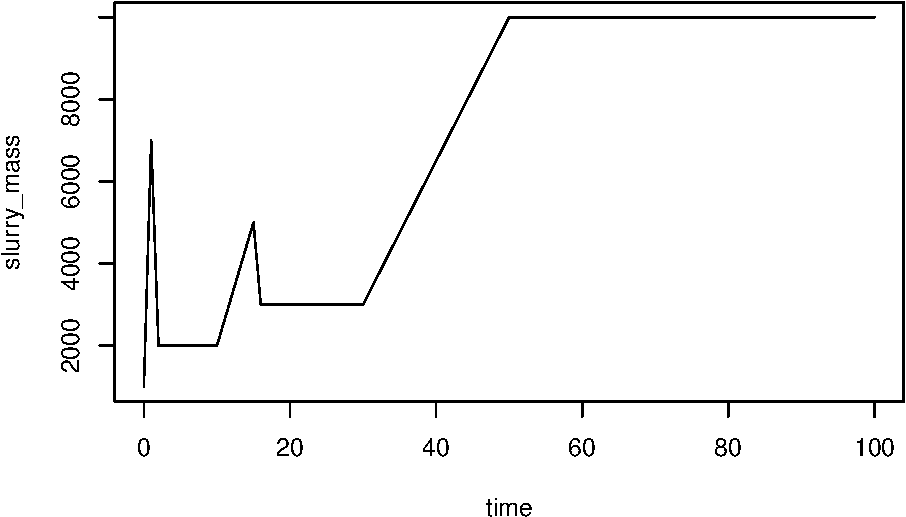
\includegraphics{simple_demo_files/figure-latex/unnamed-chunk-36-1.pdf}

\begin{Shaded}
\begin{Highlighting}[]
\FunctionTok{plot}\NormalTok{(CH4\_emis\_rate }\SpecialCharTok{\textasciitilde{}}\NormalTok{ time, }\AttributeTok{data =}\NormalTok{ out5, }\AttributeTok{type =} \StringTok{\textquotesingle{}l\textquotesingle{}}\NormalTok{)}
\end{Highlighting}
\end{Shaded}

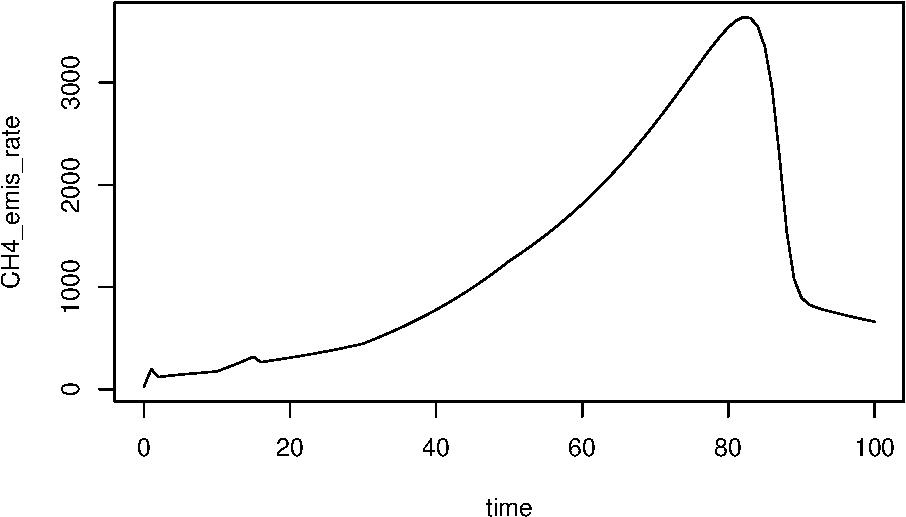
\includegraphics{simple_demo_files/figure-latex/unnamed-chunk-36-2.pdf}

\begin{Shaded}
\begin{Highlighting}[]
\FunctionTok{plot}\NormalTok{(VSd\_conc }\SpecialCharTok{\textasciitilde{}}\NormalTok{ time, }\AttributeTok{data =}\NormalTok{ out5, }\AttributeTok{type =} \StringTok{\textquotesingle{}l\textquotesingle{}}\NormalTok{)}
\end{Highlighting}
\end{Shaded}

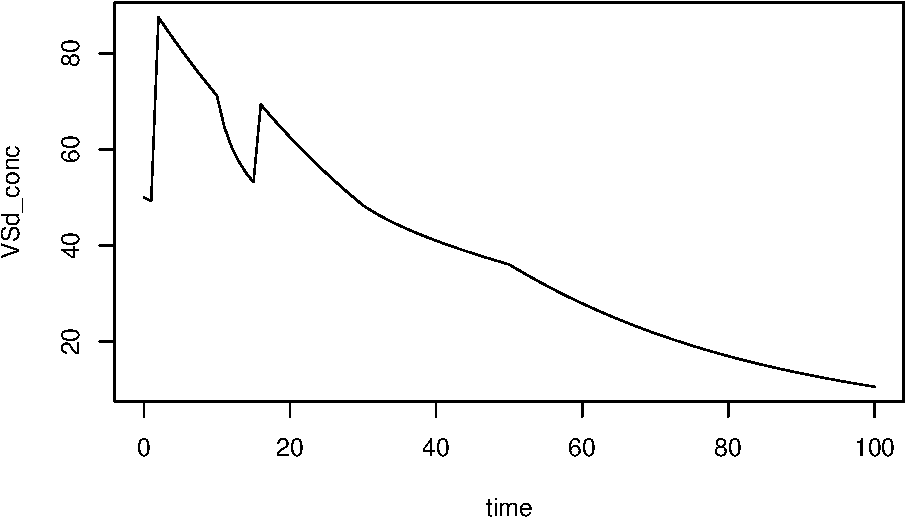
\includegraphics{simple_demo_files/figure-latex/unnamed-chunk-36-3.pdf}

\begin{Shaded}
\begin{Highlighting}[]
\FunctionTok{plot}\NormalTok{(CH3COOH\_conc }\SpecialCharTok{\textasciitilde{}}\NormalTok{ time, }\AttributeTok{data =}\NormalTok{ out5, }\AttributeTok{type =} \StringTok{\textquotesingle{}l\textquotesingle{}}\NormalTok{)}
\end{Highlighting}
\end{Shaded}

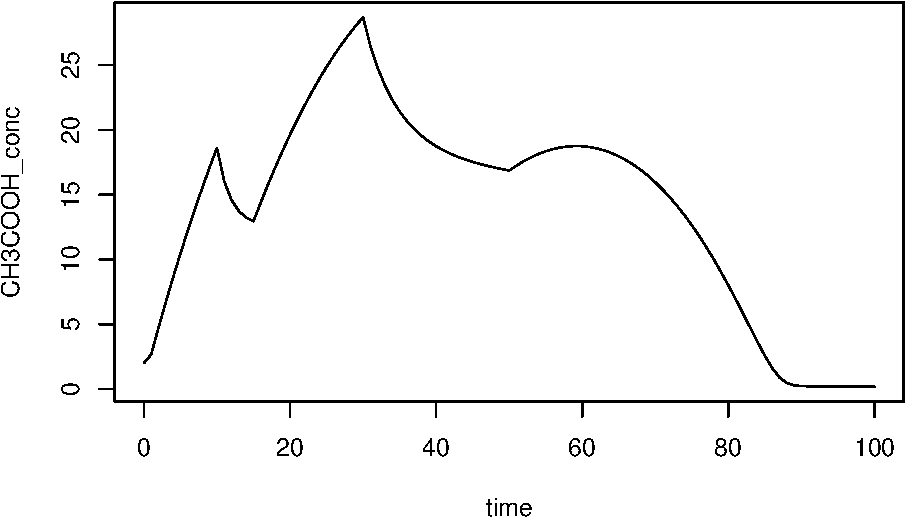
\includegraphics{simple_demo_files/figure-latex/unnamed-chunk-36-4.pdf}

\hypertarget{flexible-solutes-and-sulfate-reduction}{%
\section{6. Flexible solutes and sulfate
reduction}\label{flexible-solutes-and-sulfate-reduction}}

Any conservative solute can be added in \texttt{man\_pars}, using any
names. I am moving toward using a ``master species'' approach, so it
makes sense to use the chemical formula of the primary species, with
\texttt{p} or \texttt{m} for a charge symbol. The \texttt{comp} part of
the name below is for ``component''.

\begin{Shaded}
\begin{Highlighting}[]
\NormalTok{man\_pars6 }\OtherTok{\textless{}{-}} \FunctionTok{list}\NormalTok{(}\AttributeTok{comps =} \FunctionTok{c}\NormalTok{(}\StringTok{\textquotesingle{}H2S\textquotesingle{}}\NormalTok{, }\StringTok{\textquotesingle{}SO4m2\textquotesingle{}}\NormalTok{, }\StringTok{\textquotesingle{}NH4p\textquotesingle{}}\NormalTok{),}
                 \AttributeTok{comp\_fresh =} \FunctionTok{c}\NormalTok{(}\AttributeTok{H2S =} \FloatTok{0.01}\NormalTok{, }\AttributeTok{SO4m2 =} \FloatTok{0.2}\NormalTok{, }\AttributeTok{NH4p =} \FloatTok{2.5}\NormalTok{), }
                 \AttributeTok{VFA\_fresh =} \FunctionTok{c}\NormalTok{(}\AttributeTok{CH3COOH =} \DecValTok{2}\NormalTok{),}
                 \AttributeTok{pH =} \DecValTok{7}\NormalTok{, }\AttributeTok{dens =} \DecValTok{1000}\NormalTok{)}
\end{Highlighting}
\end{Shaded}

Note that \texttt{CH3COOH} is still special--it has a fixed name in the
code and is not conservative.

\begin{Shaded}
\begin{Highlighting}[]
\NormalTok{devtools}\SpecialCharTok{::}\FunctionTok{load\_all}\NormalTok{()}
\end{Highlighting}
\end{Shaded}

\begin{verbatim}
## i Loading ABM
\end{verbatim}

\begin{Shaded}
\begin{Highlighting}[]
\NormalTok{out6a }\OtherTok{\textless{}{-}} \FunctionTok{abm}\NormalTok{(}\DecValTok{365}\NormalTok{,}
            \AttributeTok{mng\_pars =}\NormalTok{ mng\_pars,}
            \AttributeTok{man\_pars =}\NormalTok{ man\_pars6,}
            \AttributeTok{grp\_pars =}\NormalTok{ grp\_pars,}
            \AttributeTok{mic\_pars =}\NormalTok{ mic\_pars,}
            \AttributeTok{sub\_pars =}\NormalTok{ sub\_pars,}
            \AttributeTok{chem\_pars =}\NormalTok{ chem\_pars)}
\end{Highlighting}
\end{Shaded}

\begin{verbatim}
## Warning in expandPars(pars = pars, elnms = pars$grps, parnms = grp_par_nms):
## Size-variable parameter problem: Missing element(s) in kss.
\end{verbatim}

\begin{verbatim}
## Warning in checkCOD(dat = dat, grps = pars$grps, subs = pars$subs, COD_conv =
## pars$COD_conv, : COD balance is off by 2%
\end{verbatim}

\begin{Shaded}
\begin{Highlighting}[]
\FunctionTok{tail}\NormalTok{(out6a)}
\end{Highlighting}
\end{Shaded}

\begin{verbatim}
##     time       m0       m1       m2      sr1      VSd      H2S    SO4m2    NH4p
## 364  360 74751.48 72348.85 334784.1 22188.55 15469950 115596.8 12503.17 1525000
## 365  361 76892.18 74389.05 348806.4 22374.50 15577739 117589.8 12610.22 1550000
## 366  362 79063.75 76457.33 363289.4 22556.57 15683138 119579.7 12720.29 1575000
## 367  363 81263.87 78551.47 378229.0 22734.81 15786218 121566.3 12833.71 1600000
## 368  364 83489.65 80668.67 393616.7 22909.25 15887047 123549.1 12950.88 1625000
## 369  365 85737.49 82805.50 409438.1 23079.95 15985694 125527.7 13072.29 1650000
##     CH3COOH slurry_mass CH4_emis_cum slurry_load  COD_load CH4_emis_rate temp_C
## 364 4760816      610000     26704791     3600000 187920000      124223.5     20
## 365 4650827      620000     26831123     3610000 188442000      128446.1     20
## 366 4525825      630000     26961690     3620000 188964000      132688.7     20
## 367 4385715      640000     27096499     3630000 189486000      136926.3     20
## 368 4230525      650000     27235530     3640000 190008000      141127.4     20
## 369 4060430      660000     27378729     3650000 190530000      145252.5     20
##     pH   m0_eff   m1_eff  m2_eff sr1_eff  VSd_eff  H2S_eff SO4m2_eff NH4p_eff
## 364  7 440845.9 421385.9 2227298 78898.1 53534259 561218.1  66891.92  7477500
## 365  7 440845.9 421385.9 2227298 78898.1 53534259 561218.1  66891.92  7477500
## 366  7 440845.9 421385.9 2227298 78898.1 53534259 561218.1  66891.92  7477500
## 367  7 440845.9 421385.9 2227298 78898.1 53534259 561218.1  66891.92  7477500
## 368  7 440845.9 421385.9 2227298 78898.1 53534259 561218.1  66891.92  7477500
## 369  7 440845.9 421385.9 2227298 78898.1 53534259 561218.1  66891.92  7477500
##     CH3COOH_eff slurry_mass_eff slurry_depth   m0_conc   m1_conc   m2_conc
## 364     3372964         2991000          6.1 0.1225434 0.1186047 0.5488264
## 365     3372964         2991000          6.2 0.1240196 0.1199823 0.5625909
## 366     3372964         2991000          6.3 0.1254980 0.1213608 0.5766498
## 367     3372964         2991000          6.4 0.1269748 0.1227367 0.5909829
## 368     3372964         2991000          6.5 0.1284456 0.1241056 0.6055642
## 369     3372964         2991000          6.6 0.1299053 0.1254629 0.6203607
##       sr1_conc VSd_conc  H2S_conc SO4m2_conc NH4p_conc CH3COOH_conc m0_eff_conc
## 364 0.03637467 25.36057 0.1895030 0.02049700       2.5     7.804616   0.1473908
## 365 0.03608791 25.12539 0.1896609 0.02033907       2.5     7.501334   0.1473908
## 366 0.03580408 24.89387 0.1898091 0.02019094       2.5     7.183849   0.1473908
## 367 0.03552313 24.66596 0.1899473 0.02005267       2.5     6.852680   0.1473908
## 368 0.03524500 24.44161 0.1900756 0.01992443       2.5     6.508500   0.1473908
## 369 0.03496962 24.22075 0.1901935 0.01980650       2.5     6.152166   0.1473908
##     m1_eff_conc m2_eff_conc sr1_eff_conc VSd_eff_conc H2S_eff_conc
## 364   0.1408846   0.7446668    0.0263785     17.89845    0.1876356
## 365   0.1408846   0.7446668    0.0263785     17.89845    0.1876356
## 366   0.1408846   0.7446668    0.0263785     17.89845    0.1876356
## 367   0.1408846   0.7446668    0.0263785     17.89845    0.1876356
## 368   0.1408846   0.7446668    0.0263785     17.89845    0.1876356
## 369   0.1408846   0.7446668    0.0263785     17.89845    0.1876356
##     SO4m2_eff_conc NH4p_eff_conc CH3COOH_eff_conc
## 364      0.0223644           2.5         1.127704
## 365      0.0223644           2.5         1.127704
## 366      0.0223644           2.5         1.127704
## 367      0.0223644           2.5         1.127704
## 368      0.0223644           2.5         1.127704
## 369      0.0223644           2.5         1.127704
\end{verbatim}

\begin{Shaded}
\begin{Highlighting}[]
\FunctionTok{head}\NormalTok{(out6a)}
\end{Highlighting}
\end{Shaded}

\begin{verbatim}
##   time        m0        m1        m2       sr1       VSd       H2S    SO4m2
## 1    0   50.0000   50.0000   50.0000   50.0000   50000.0   10.0000  200.000
## 2    1  553.9977  553.8414  558.3574  555.0147  542318.5  268.9637 2041.036
## 3    2 1066.2080 1065.6056 1083.0938 1067.9792 1022077.4  788.7361 3621.264
## 4    3 1588.1329 1586.7628 1626.7495 1587.7198 1489599.2 1554.5640 4955.436
## 5    4 2120.8456 2118.3596 2191.3257 2112.6512 1945197.9 2545.3729 6064.627
## 6    5 2665.1817 2661.2072 2778.5446 2641.0154 2389179.5 3737.1169 6972.883
##     NH4p   CH3COOH slurry_mass CH4_emis_cum slurry_load COD_load CH4_emis_rate
## 1   2500   2000.00        1000       0.0000           0        0      25.52844
## 2  27500  28849.48       11000     163.4287       10000   522000     308.15048
## 3  52500  66757.26       21000     627.6723       20000  1044000     625.17882
## 4  77500 115293.28       31000    1422.3638       30000  1566000     968.06890
## 5 102500 174068.44       41000    2570.9586       40000  2088000    1332.46915
## 6 127500 242718.37       51000    4093.6840       50000  2610000    1716.05164
##   temp_C pH m0_eff m1_eff m2_eff sr1_eff VSd_eff H2S_eff SO4m2_eff NH4p_eff
## 1     20  7      0      0      0       0       0       0         0        0
## 2     20  7      0      0      0       0       0       0         0        0
## 3     20  7      0      0      0       0       0       0         0        0
## 4     20  7      0      0      0       0       0       0         0        0
## 5     20  7      0      0      0       0       0       0         0        0
## 6     20  7      0      0      0       0       0       0         0        0
##   CH3COOH_eff slurry_mass_eff slurry_depth    m0_conc    m1_conc    m2_conc
## 1           0               0         0.01 0.05000000 0.05000000 0.05000000
## 2           0               0         0.11 0.05036343 0.05034921 0.05075976
## 3           0               0         0.21 0.05077181 0.05074312 0.05157589
## 4           0               0         0.31 0.05123009 0.05118590 0.05247579
## 5           0               0         0.41 0.05172794 0.05166731 0.05344697
## 6           0               0         0.51 0.05225847 0.05218053 0.05448127
##     sr1_conc VSd_conc   H2S_conc SO4m2_conc NH4p_conc CH3COOH_conc m0_eff_conc
## 1 0.05000000 50.00000 0.01000000  0.2000000       2.5     2.000000         NaN
## 2 0.05045588 49.30168 0.02445125  0.1855488       2.5     2.622680         NaN
## 3 0.05085615 48.67035 0.03755886  0.1724411       2.5     3.178917         NaN
## 4 0.05121677 48.05159 0.05014723  0.1598528       2.5     3.719138         NaN
## 5 0.05152808 47.44385 0.06208226  0.1479177       2.5     4.245572         NaN
## 6 0.05178462 46.84666 0.07327680  0.1367232       2.5     4.759184         NaN
##   m1_eff_conc m2_eff_conc sr1_eff_conc VSd_eff_conc H2S_eff_conc SO4m2_eff_conc
## 1         NaN         NaN          NaN          NaN          NaN            NaN
## 2         NaN         NaN          NaN          NaN          NaN            NaN
## 3         NaN         NaN          NaN          NaN          NaN            NaN
## 4         NaN         NaN          NaN          NaN          NaN            NaN
## 5         NaN         NaN          NaN          NaN          NaN            NaN
## 6         NaN         NaN          NaN          NaN          NaN            NaN
##   NH4p_eff_conc CH3COOH_eff_conc
## 1           NaN              NaN
## 2           NaN              NaN
## 3           NaN              NaN
## 4           NaN              NaN
## 5           NaN              NaN
## 6           NaN              NaN
\end{verbatim}

Conservative components are boring in output (without inhibition or
volatilization).

\begin{Shaded}
\begin{Highlighting}[]
\FunctionTok{plot}\NormalTok{(NH4p\_conc }\SpecialCharTok{\textasciitilde{}}\NormalTok{ time, }\AttributeTok{data =}\NormalTok{ out6a)}
\end{Highlighting}
\end{Shaded}

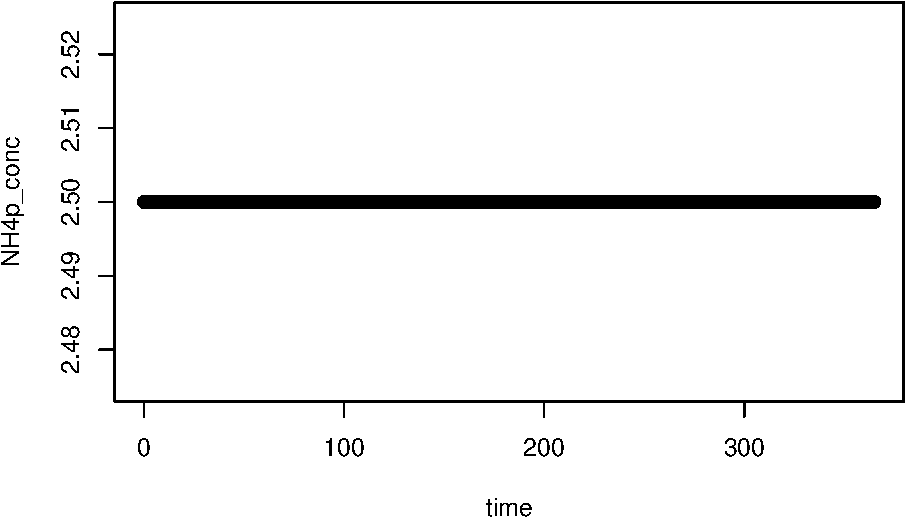
\includegraphics{simple_demo_files/figure-latex/unnamed-chunk-40-1.pdf}

\begin{Shaded}
\begin{Highlighting}[]
\FunctionTok{plot}\NormalTok{(NH4p }\SpecialCharTok{\textasciitilde{}}\NormalTok{ time, }\AttributeTok{data =}\NormalTok{ out6a)}
\end{Highlighting}
\end{Shaded}

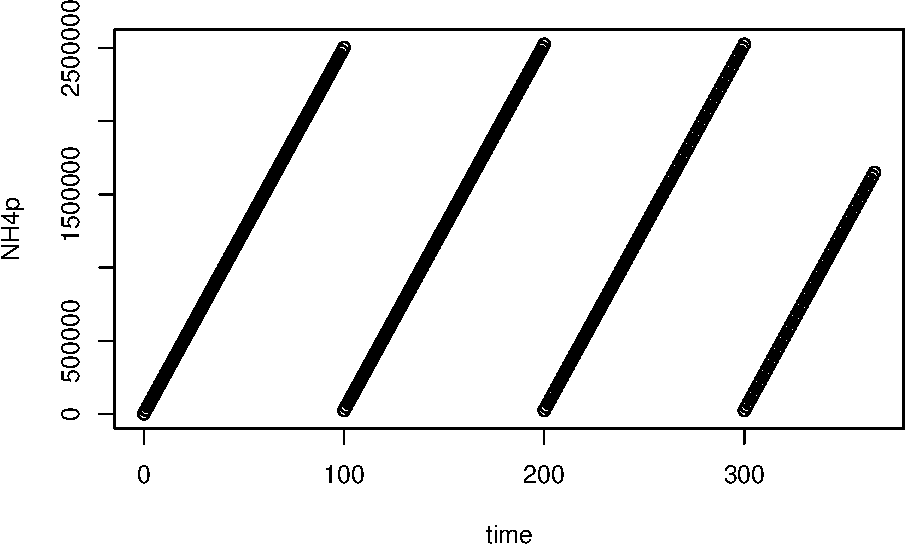
\includegraphics{simple_demo_files/figure-latex/unnamed-chunk-40-2.pdf}

But now with sulfate and sulfide, sulfate reducers can grow.

\begin{Shaded}
\begin{Highlighting}[]
\FunctionTok{plot}\NormalTok{(sr1\_conc }\SpecialCharTok{\textasciitilde{}}\NormalTok{ time, }\AttributeTok{data =}\NormalTok{ out6a, }\AttributeTok{type =} \StringTok{\textquotesingle{}l\textquotesingle{}}\NormalTok{, }\AttributeTok{ylim =} \FunctionTok{c}\NormalTok{(}\DecValTok{0}\NormalTok{, }\FloatTok{0.4}\NormalTok{))}
\FunctionTok{lines}\NormalTok{(m1\_conc }\SpecialCharTok{\textasciitilde{}}\NormalTok{ time, }\AttributeTok{data =}\NormalTok{ out6a, }\AttributeTok{col =} \StringTok{\textquotesingle{}red\textquotesingle{}}\NormalTok{)}
\end{Highlighting}
\end{Shaded}

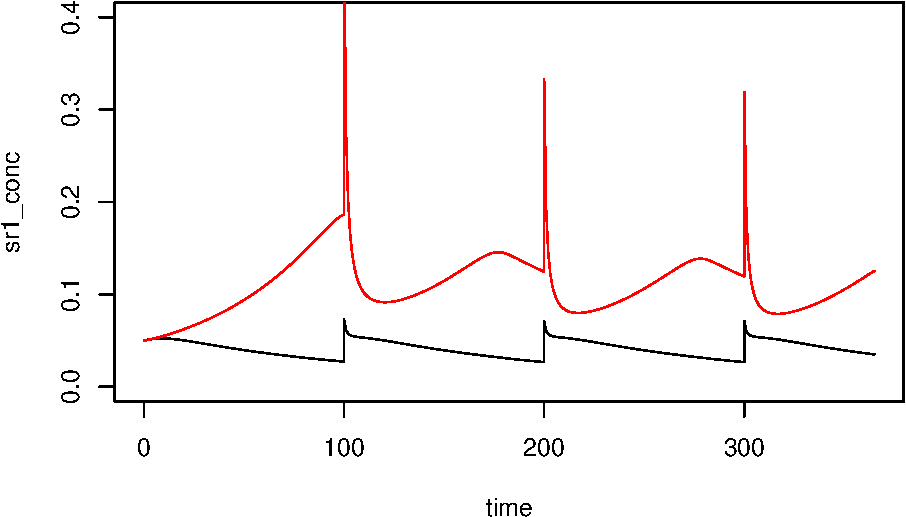
\includegraphics{simple_demo_files/figure-latex/unnamed-chunk-41-1.pdf}

And if H2S is a component, it will be produced.

\begin{Shaded}
\begin{Highlighting}[]
\FunctionTok{plot}\NormalTok{(SO4m2\_conc }\SpecialCharTok{\textasciitilde{}}\NormalTok{ time, }\AttributeTok{data =}\NormalTok{ out6a, }\AttributeTok{type =} \StringTok{\textquotesingle{}l\textquotesingle{}}\NormalTok{)}
\end{Highlighting}
\end{Shaded}

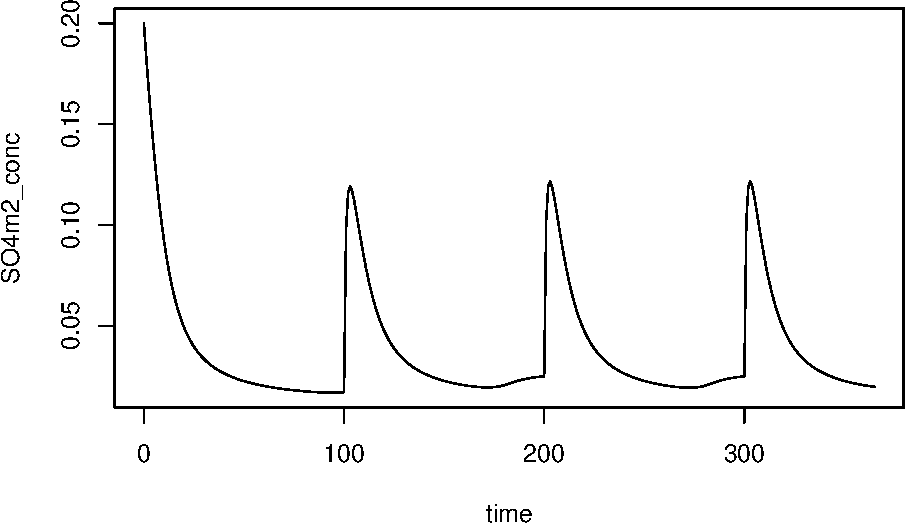
\includegraphics{simple_demo_files/figure-latex/unnamed-chunk-42-1.pdf}

\begin{Shaded}
\begin{Highlighting}[]
\FunctionTok{plot}\NormalTok{(H2S\_conc }\SpecialCharTok{\textasciitilde{}}\NormalTok{ time, }\AttributeTok{data =}\NormalTok{ out6a, }\AttributeTok{type =} \StringTok{\textquotesingle{}l\textquotesingle{}}\NormalTok{)}
\end{Highlighting}
\end{Shaded}

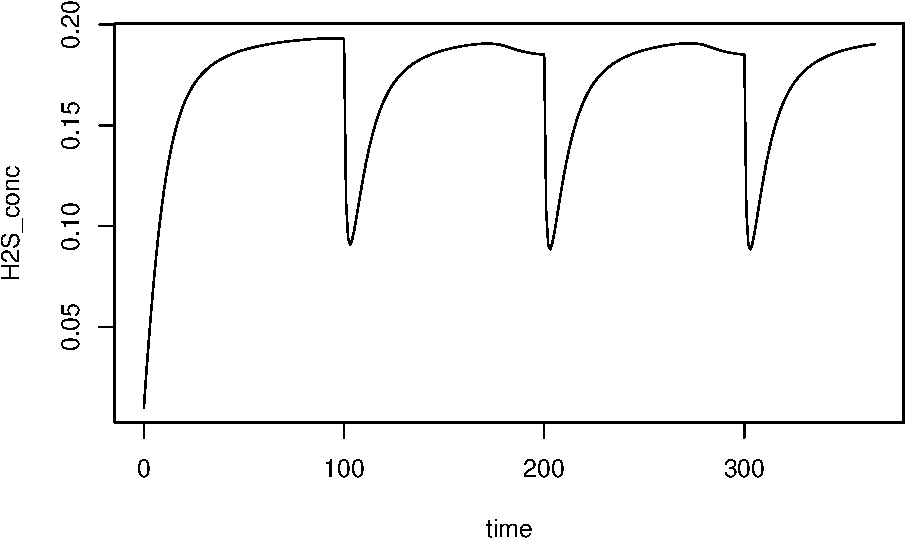
\includegraphics{simple_demo_files/figure-latex/unnamed-chunk-42-2.pdf}

We can see dilution effects at if some washing water is added.

\begin{Shaded}
\begin{Highlighting}[]
\NormalTok{mng\_pars6 }\OtherTok{=} \FunctionTok{list}\NormalTok{(}\AttributeTok{slurry\_prod\_rate =} \DecValTok{10000}\NormalTok{, }
                \AttributeTok{slurry\_mass =} \DecValTok{1000}\NormalTok{,     }
                \AttributeTok{storage\_depth =} \DecValTok{2}\NormalTok{,     }
                \AttributeTok{resid\_depth =} \FloatTok{0.1}\NormalTok{,      }
                \AttributeTok{area =} \DecValTok{100}\NormalTok{,              }
                \AttributeTok{empty\_int =} \DecValTok{100}\NormalTok{,          }
                \AttributeTok{temp\_C =} \DecValTok{20}\NormalTok{,}
                \AttributeTok{wash\_water =} \DecValTok{100000}\NormalTok{,            }
                \AttributeTok{wash\_int =} \DecValTok{100}\NormalTok{,}
                \AttributeTok{rest\_d =} \DecValTok{0}\NormalTok{,}
                \AttributeTok{resid\_enrich =} \DecValTok{1}\NormalTok{)}
\end{Highlighting}
\end{Shaded}

\begin{Shaded}
\begin{Highlighting}[]
\NormalTok{out6b }\OtherTok{\textless{}{-}} \FunctionTok{abm}\NormalTok{(}\DecValTok{365}\NormalTok{,}
            \AttributeTok{mng\_pars =}\NormalTok{ mng\_pars6,}
            \AttributeTok{man\_pars =}\NormalTok{ man\_pars6,}
            \AttributeTok{grp\_pars =}\NormalTok{ grp\_pars,}
            \AttributeTok{mic\_pars =}\NormalTok{ mic\_pars,}
            \AttributeTok{sub\_pars =}\NormalTok{ sub\_pars,}
            \AttributeTok{chem\_pars =}\NormalTok{ chem\_pars)}
\end{Highlighting}
\end{Shaded}

\begin{verbatim}
## Warning in expandPars(pars = pars, elnms = pars$grps, parnms = grp_par_nms):
## Size-variable parameter problem: Missing element(s) in kss.
\end{verbatim}

\begin{verbatim}
## Warning in checkCOD(dat = dat, grps = pars$grps, subs = pars$subs, COD_conv =
## pars$COD_conv, : COD balance is off by 32%
\end{verbatim}

\begin{Shaded}
\begin{Highlighting}[]
\FunctionTok{plot}\NormalTok{(NH4p\_conc }\SpecialCharTok{\textasciitilde{}}\NormalTok{ time, }\AttributeTok{data =}\NormalTok{ out6b, }\AttributeTok{type =} \StringTok{\textquotesingle{}l\textquotesingle{}}\NormalTok{)}
\FunctionTok{lines}\NormalTok{(NH4p\_conc }\SpecialCharTok{\textasciitilde{}}\NormalTok{ time, }\AttributeTok{data =}\NormalTok{ out6a, }\AttributeTok{col =} \StringTok{\textquotesingle{}red\textquotesingle{}}\NormalTok{)}
\end{Highlighting}
\end{Shaded}

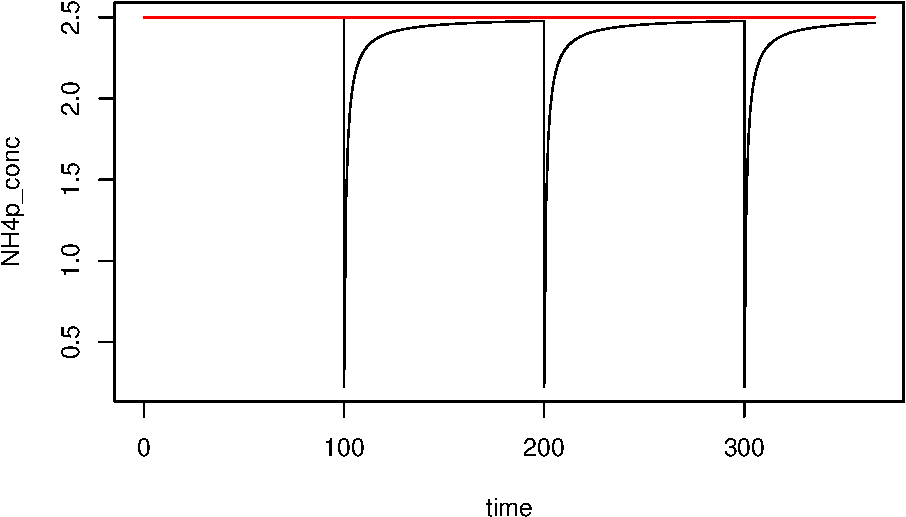
\includegraphics{simple_demo_files/figure-latex/unnamed-chunk-45-1.pdf}

To include sulfate reduction, there must be an \texttt{sr} microbial
group and \texttt{SO4m2} must be a chemical component. Omit either to
exclude sulfate reduction.

\begin{Shaded}
\begin{Highlighting}[]
\NormalTok{man\_pars6c }\OtherTok{\textless{}{-}} \FunctionTok{list}\NormalTok{(}\AttributeTok{comps =} \FunctionTok{c}\NormalTok{(}\StringTok{\textquotesingle{}H2S\textquotesingle{}}\NormalTok{, }\StringTok{\textquotesingle{}NH4p\textquotesingle{}}\NormalTok{),}
                 \AttributeTok{comp\_fresh =} \FunctionTok{c}\NormalTok{(}\AttributeTok{H2S =} \FloatTok{0.01}\NormalTok{, }\AttributeTok{NH4p =} \FloatTok{2.5}\NormalTok{), }
                 \AttributeTok{VFA\_fresh =} \FunctionTok{c}\NormalTok{(}\AttributeTok{CH3COOH =} \DecValTok{2}\NormalTok{),}
                 \AttributeTok{pH =} \DecValTok{7}\NormalTok{, }\AttributeTok{dens =} \DecValTok{1000}\NormalTok{)}
\end{Highlighting}
\end{Shaded}

\begin{Shaded}
\begin{Highlighting}[]
\NormalTok{grp\_pars6c }\OtherTok{\textless{}{-}} \FunctionTok{list}\NormalTok{(}\AttributeTok{grps =} \FunctionTok{c}\NormalTok{(}\StringTok{\textquotesingle{}m0\textquotesingle{}}\NormalTok{, }\StringTok{\textquotesingle{}m1\textquotesingle{}}\NormalTok{, }\StringTok{\textquotesingle{}m2\textquotesingle{}}\NormalTok{),}
                 \AttributeTok{yield =} \FunctionTok{c}\NormalTok{(}\AttributeTok{default =} \FloatTok{0.05}\NormalTok{),}
                 \AttributeTok{xa\_fresh =} \FunctionTok{c}\NormalTok{(}\AttributeTok{all =} \FloatTok{0.05}\NormalTok{),}
                 \AttributeTok{xa\_init =} \FunctionTok{c}\NormalTok{(}\AttributeTok{all =} \FloatTok{0.05}\NormalTok{),}
                 \AttributeTok{dd\_rate =} \FunctionTok{c}\NormalTok{(}\AttributeTok{all =} \FloatTok{0.02}\NormalTok{),}
                 \AttributeTok{ksv =} \FunctionTok{c}\NormalTok{(}\AttributeTok{default =} \DecValTok{1}\NormalTok{),}
                 \AttributeTok{qhat\_opt =} \FunctionTok{c}\NormalTok{(}\AttributeTok{m0 =} \DecValTok{1}\NormalTok{, }\AttributeTok{m1 =} \DecValTok{1}\NormalTok{, }\AttributeTok{m2 =} \DecValTok{2}\NormalTok{),}
                 \AttributeTok{T\_opt =} \FunctionTok{c}\NormalTok{(}\AttributeTok{m0 =} \DecValTok{18}\NormalTok{, }\AttributeTok{m1 =} \DecValTok{18}\NormalTok{, }\AttributeTok{m2 =} \DecValTok{28}\NormalTok{),}
                 \AttributeTok{T\_min =} \FunctionTok{c}\NormalTok{(}\AttributeTok{m0 =} \DecValTok{0}\NormalTok{, }\AttributeTok{m1 =} \FloatTok{6.41}\NormalTok{, }\AttributeTok{m2 =} \FloatTok{6.41}\NormalTok{),}
                 \AttributeTok{T\_max =} \FunctionTok{c}\NormalTok{(}\AttributeTok{m0 =} \DecValTok{25}\NormalTok{, }\AttributeTok{m1 =} \DecValTok{25}\NormalTok{, }\AttributeTok{m2 =} \DecValTok{38}\NormalTok{))}
\end{Highlighting}
\end{Shaded}

\begin{Shaded}
\begin{Highlighting}[]
\NormalTok{devtools}\SpecialCharTok{::}\FunctionTok{load\_all}\NormalTok{()}
\end{Highlighting}
\end{Shaded}

\begin{verbatim}
## i Loading ABM
\end{verbatim}

\begin{Shaded}
\begin{Highlighting}[]
\NormalTok{out6c }\OtherTok{\textless{}{-}} \FunctionTok{abm}\NormalTok{(}\DecValTok{365}\NormalTok{,}
            \AttributeTok{mng\_pars =}\NormalTok{ mng\_pars6,}
            \AttributeTok{man\_pars =}\NormalTok{ man\_pars6c,}
            \AttributeTok{grp\_pars =}\NormalTok{ grp\_pars6c,}
            \AttributeTok{mic\_pars =}\NormalTok{ mic\_pars,}
            \AttributeTok{sub\_pars =}\NormalTok{ sub\_pars,}
            \AttributeTok{chem\_pars =}\NormalTok{ chem\_pars)}
\end{Highlighting}
\end{Shaded}

\begin{verbatim}
## Warning in checkCOD(dat = dat, grps = pars$grps, subs = pars$subs, COD_conv =
## pars$COD_conv, : COD balance is off by 32%
\end{verbatim}

\begin{Shaded}
\begin{Highlighting}[]
\FunctionTok{plot}\NormalTok{(CH4\_emis\_cum }\SpecialCharTok{\textasciitilde{}}\NormalTok{ time, }\AttributeTok{data =}\NormalTok{ out6a, }\AttributeTok{type =} \StringTok{\textquotesingle{}l\textquotesingle{}}\NormalTok{)}
\FunctionTok{lines}\NormalTok{(CH4\_emis\_cum }\SpecialCharTok{\textasciitilde{}}\NormalTok{ time, }\AttributeTok{data =}\NormalTok{ out6c, }\AttributeTok{col =} \StringTok{\textquotesingle{}red\textquotesingle{}}\NormalTok{)}
\end{Highlighting}
\end{Shaded}

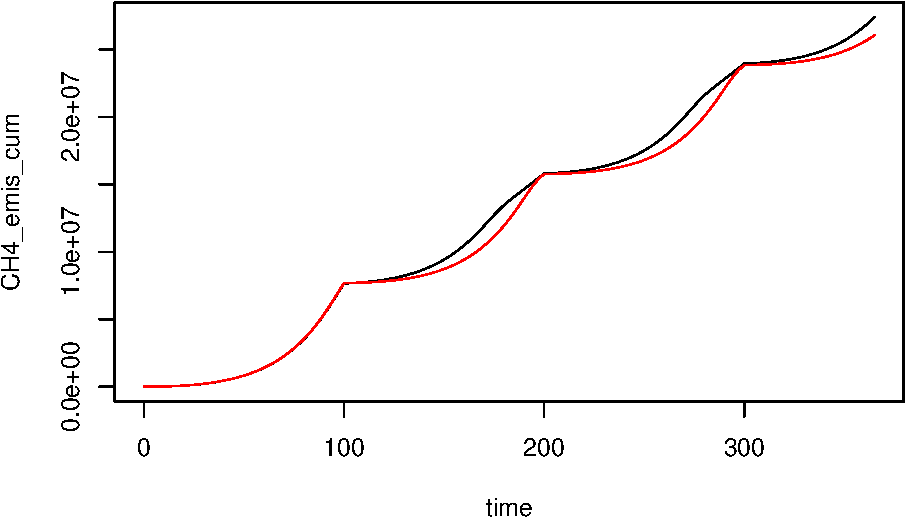
\includegraphics{simple_demo_files/figure-latex/unnamed-chunk-49-1.pdf}

\begin{Shaded}
\begin{Highlighting}[]
\FunctionTok{plot}\NormalTok{(CH3COOH\_conc }\SpecialCharTok{\textasciitilde{}}\NormalTok{ time, }\AttributeTok{data =}\NormalTok{ out6a, }\AttributeTok{type =} \StringTok{\textquotesingle{}l\textquotesingle{}}\NormalTok{)}
\FunctionTok{lines}\NormalTok{(CH3COOH\_conc }\SpecialCharTok{\textasciitilde{}}\NormalTok{ time, }\AttributeTok{data =}\NormalTok{ out6c, }\AttributeTok{col =} \StringTok{\textquotesingle{}red\textquotesingle{}}\NormalTok{)}
\end{Highlighting}
\end{Shaded}

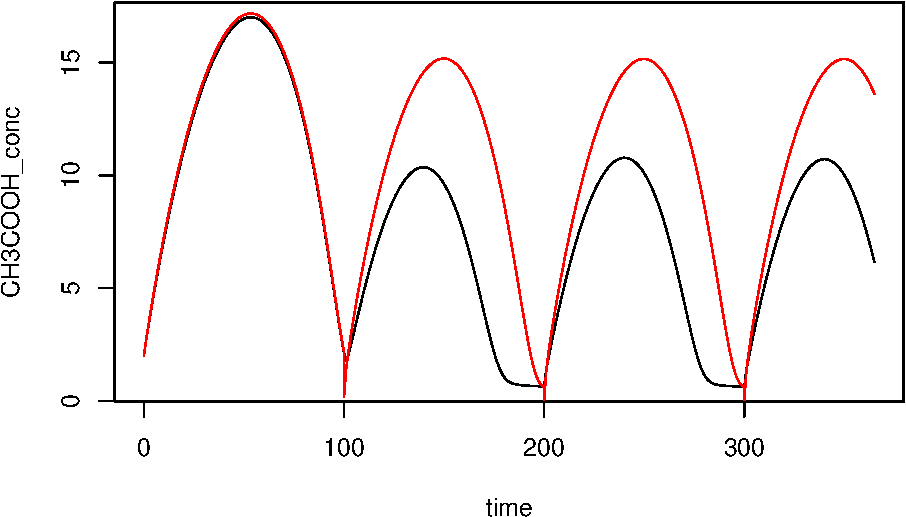
\includegraphics{simple_demo_files/figure-latex/unnamed-chunk-50-1.pdf}

\begin{Shaded}
\begin{Highlighting}[]
\FunctionTok{plot}\NormalTok{(m1\_conc }\SpecialCharTok{\textasciitilde{}}\NormalTok{ time, }\AttributeTok{data =}\NormalTok{ out6a, }\AttributeTok{type =} \StringTok{\textquotesingle{}l\textquotesingle{}}\NormalTok{)}
\FunctionTok{lines}\NormalTok{(m1\_conc }\SpecialCharTok{\textasciitilde{}}\NormalTok{ time, }\AttributeTok{data =}\NormalTok{ out6c, }\AttributeTok{col =} \StringTok{\textquotesingle{}red\textquotesingle{}}\NormalTok{)}
\end{Highlighting}
\end{Shaded}

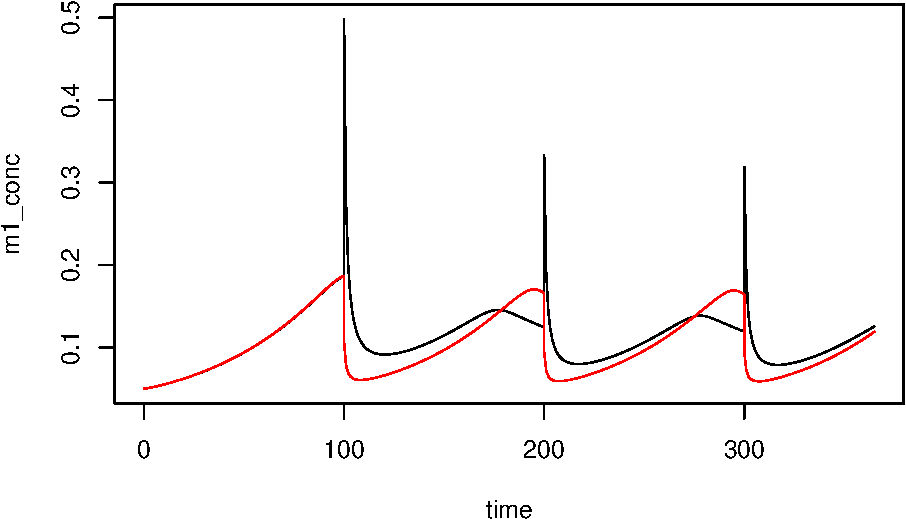
\includegraphics{simple_demo_files/figure-latex/unnamed-chunk-51-1.pdf}

\begin{Shaded}
\begin{Highlighting}[]
\FunctionTok{plot}\NormalTok{(slurry\_mass }\SpecialCharTok{\textasciitilde{}}\NormalTok{ time, }\AttributeTok{data =}\NormalTok{ out6a, }\AttributeTok{type =} \StringTok{\textquotesingle{}l\textquotesingle{}}\NormalTok{)}
\FunctionTok{lines}\NormalTok{(slurry\_mass }\SpecialCharTok{\textasciitilde{}}\NormalTok{ time, }\AttributeTok{data =}\NormalTok{ out6c, }\AttributeTok{col =} \StringTok{\textquotesingle{}red\textquotesingle{}}\NormalTok{)}
\end{Highlighting}
\end{Shaded}

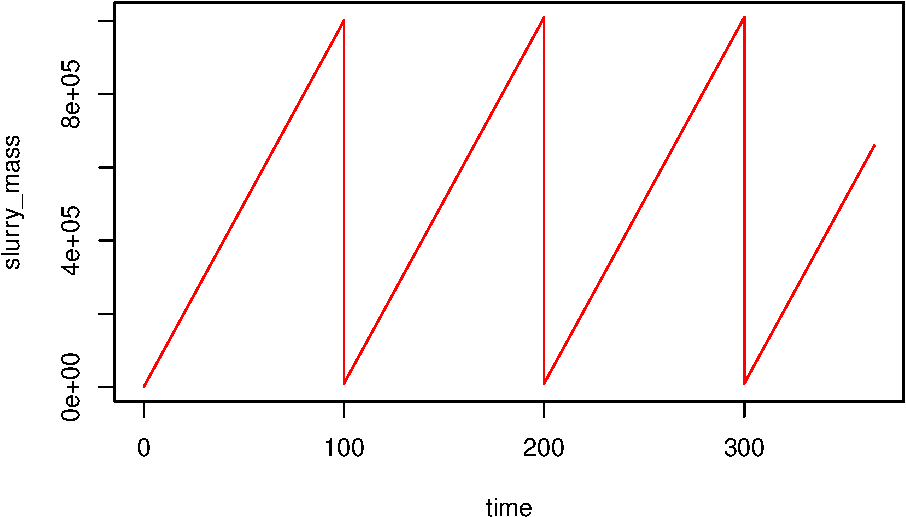
\includegraphics{simple_demo_files/figure-latex/unnamed-chunk-52-1.pdf}

\hypertarget{speciation}{%
\section{7. Speciation}\label{speciation}}

Acid-base reactions are needed for inhibition and for CO2 emission. They
can be added for any component. The \texttt{chem\_pars} argument can
accept temperature-dependent log ka expressions. Use \texttt{temp\_K}
for absolute temperature in those expressions.

\begin{Shaded}
\begin{Highlighting}[]
\NormalTok{man\_pars7 }\OtherTok{\textless{}{-}} \FunctionTok{list}\NormalTok{(}\AttributeTok{comps =} \FunctionTok{c}\NormalTok{(}\StringTok{\textquotesingle{}H2S\textquotesingle{}}\NormalTok{, }\StringTok{\textquotesingle{}NH4p\textquotesingle{}}\NormalTok{),}
                 \AttributeTok{comp\_fresh =} \FunctionTok{c}\NormalTok{(}\AttributeTok{H2S =} \FloatTok{0.01}\NormalTok{, }\AttributeTok{NH4p =} \FloatTok{2.5}\NormalTok{), }
                 \AttributeTok{VFA\_fresh =} \FunctionTok{c}\NormalTok{(}\AttributeTok{CH3COOH =} \DecValTok{2}\NormalTok{),}
                 \AttributeTok{pH =} \DecValTok{7}\NormalTok{, }\AttributeTok{dens =} \DecValTok{1000}\NormalTok{)}

\NormalTok{chem\_pars7 }\OtherTok{\textless{}{-}} \FunctionTok{list}\NormalTok{(}\AttributeTok{COD\_conv =} \FunctionTok{c}\NormalTok{(}\AttributeTok{CH4 =} \DecValTok{1}\SpecialCharTok{/}\FloatTok{0.2507}\NormalTok{, }\AttributeTok{xa =} \DecValTok{1}\SpecialCharTok{/}\FloatTok{0.7069561}\NormalTok{,}
                               \AttributeTok{VFA =} \DecValTok{1}\SpecialCharTok{/}\FloatTok{0.9383125}\NormalTok{, }\AttributeTok{S =} \DecValTok{1}\SpecialCharTok{/}\FloatTok{0.5015}\NormalTok{, }\AttributeTok{VS =} \DecValTok{1}\SpecialCharTok{/}\FloatTok{0.69}\NormalTok{, }
                               \AttributeTok{CO2\_aer =} \DecValTok{1}\SpecialCharTok{/}\FloatTok{0.436}\NormalTok{, }\AttributeTok{CO2\_sr =} \DecValTok{1}\SpecialCharTok{/}\FloatTok{1.2}\NormalTok{, }
                               \AttributeTok{C\_xa =} \DecValTok{1}\SpecialCharTok{/}\FloatTok{0.3753125}\NormalTok{),}
                   \AttributeTok{specs =} \FunctionTok{c}\NormalTok{(}\StringTok{\textquotesingle{}NH3\textquotesingle{}}\NormalTok{, }\StringTok{\textquotesingle{}HSm\textquotesingle{}}\NormalTok{, }\StringTok{\textquotesingle{}CH3COOm\textquotesingle{}}\NormalTok{),}
                   \AttributeTok{mspec =} \FunctionTok{c}\NormalTok{(}\AttributeTok{NH3 =} \StringTok{\textquotesingle{}NH4p\textquotesingle{}}\NormalTok{, }\AttributeTok{HSm =} \StringTok{\textquotesingle{}H2S\textquotesingle{}}\NormalTok{, }\AttributeTok{CH3COOm =} \StringTok{\textquotesingle{}CH3COOH\textquotesingle{}}\NormalTok{),}
                   \AttributeTok{lka =} \FunctionTok{c}\NormalTok{(}\AttributeTok{NH3 =} \StringTok{\textquotesingle{}{-} 0.09046 {-} 2729.31/temp\_K\textquotesingle{}}\NormalTok{, }
                           \AttributeTok{HSm =} \StringTok{\textquotesingle{}{-} 3448.7/temp\_K + 47.479 {-} 7.5227 * log(temp\_K)\textquotesingle{}}\NormalTok{,}
                           \AttributeTok{CH3COOm =} \StringTok{\textquotesingle{}{-} 4.8288 + 21.42/temp\_K\textquotesingle{}}\NormalTok{)}
\NormalTok{)}
\end{Highlighting}
\end{Shaded}

Here \texttt{comps} are the chemical ``components'', or ``master
species'', as described a bit above. All are automatically included as
chemical species in \texttt{packPars()}. In the \texttt{chem\_pars}
argument, \texttt{specs} are the other (non-master) species that the
master species are in equilirbium with. And \texttt{mspec} are the
associated master species. So the NH3 species comes from NH4+. When
there is speciation, the master species are always taken as the
protonated ones. So the species in \texttt{specs} always have one less
proton than their associated master species. Only 2 species are
supported for any component (master species and one more).

\begin{Shaded}
\begin{Highlighting}[]
\NormalTok{devtools}\SpecialCharTok{::}\FunctionTok{load\_all}\NormalTok{()}
\end{Highlighting}
\end{Shaded}

\begin{verbatim}
## i Loading ABM
\end{verbatim}

\begin{Shaded}
\begin{Highlighting}[]
\NormalTok{out7 }\OtherTok{\textless{}{-}} \FunctionTok{abm}\NormalTok{(}\DecValTok{365}\NormalTok{,}
            \AttributeTok{mng\_pars =}\NormalTok{ mng\_pars,}
            \AttributeTok{man\_pars =}\NormalTok{ man\_pars6,}
            \AttributeTok{grp\_pars =}\NormalTok{ grp\_pars,}
            \AttributeTok{mic\_pars =}\NormalTok{ mic\_pars,}
            \AttributeTok{sub\_pars =}\NormalTok{ sub\_pars,}
            \AttributeTok{chem\_pars =}\NormalTok{ chem\_pars7)}
\end{Highlighting}
\end{Shaded}

\begin{verbatim}
## Warning in expandPars(pars = pars, elnms = pars$grps, parnms = grp_par_nms):
## Size-variable parameter problem: Missing element(s) in kss.
\end{verbatim}

\begin{verbatim}
## Warning in checkCOD(dat = dat, grps = pars$grps, subs = pars$subs, COD_conv =
## pars$COD_conv, : COD balance is off by 2%
\end{verbatim}

\begin{Shaded}
\begin{Highlighting}[]
\FunctionTok{head}\NormalTok{(out7)}
\end{Highlighting}
\end{Shaded}

\begin{verbatim}
##   time        m0        m1        m2       sr1       VSd       H2S    SO4m2
## 1    0   50.0000   50.0000   50.0000   50.0000   50000.0   10.0000  200.000
## 2    1  553.9977  553.8414  558.3574  555.0147  542318.5  268.9637 2041.036
## 3    2 1066.2080 1065.6056 1083.0938 1067.9792 1022077.4  788.7361 3621.264
## 4    3 1588.1329 1586.7628 1626.7495 1587.7198 1489599.2 1554.5640 4955.436
## 5    4 2120.8456 2118.3596 2191.3257 2112.6512 1945197.9 2545.3729 6064.627
## 6    5 2665.1817 2661.2072 2778.5446 2641.0154 2389179.5 3737.1169 6972.883
##     NH4p   CH3COOH slurry_mass CH4_emis_cum slurry_load COD_load CH4_emis_rate
## 1   2500   2000.00        1000       0.0000           0        0      25.52844
## 2  27500  28849.48       11000     163.4287       10000   522000     308.15048
## 3  52500  66757.26       21000     627.6723       20000  1044000     625.17882
## 4  77500 115293.28       31000    1422.3638       30000  1566000     968.06890
## 5 102500 174068.44       41000    2570.9586       40000  2088000    1332.46915
## 6 127500 242718.37       51000    4093.6840       50000  2610000    1716.05164
##   temp_C pH m0_eff m1_eff m2_eff sr1_eff VSd_eff H2S_eff SO4m2_eff NH4p_eff
## 1     20  7      0      0      0       0       0       0         0        0
## 2     20  7      0      0      0       0       0       0         0        0
## 3     20  7      0      0      0       0       0       0         0        0
## 4     20  7      0      0      0       0       0       0         0        0
## 5     20  7      0      0      0       0       0       0         0        0
## 6     20  7      0      0      0       0       0       0         0        0
##   CH3COOH_eff slurry_mass_eff slurry_depth    m0_conc    m1_conc    m2_conc
## 1           0               0         0.01 0.05000000 0.05000000 0.05000000
## 2           0               0         0.11 0.05036343 0.05034921 0.05075976
## 3           0               0         0.21 0.05077181 0.05074312 0.05157589
## 4           0               0         0.31 0.05123009 0.05118590 0.05247579
## 5           0               0         0.41 0.05172794 0.05166731 0.05344697
## 6           0               0         0.51 0.05225847 0.05218053 0.05448127
##     sr1_conc VSd_conc   H2S_conc SO4m2_conc NH4p_conc CH3COOH_conc m0_eff_conc
## 1 0.05000000 50.00000 0.01000000  0.2000000       2.5     2.000000         NaN
## 2 0.05045588 49.30168 0.02445125  0.1855488       2.5     2.622680         NaN
## 3 0.05085615 48.67035 0.03755886  0.1724411       2.5     3.178917         NaN
## 4 0.05121677 48.05159 0.05014723  0.1598528       2.5     3.719138         NaN
## 5 0.05152808 47.44385 0.06208226  0.1479177       2.5     4.245572         NaN
## 6 0.05178462 46.84666 0.07327680  0.1367232       2.5     4.759184         NaN
##   m1_eff_conc m2_eff_conc sr1_eff_conc VSd_eff_conc H2S_eff_conc SO4m2_eff_conc
## 1         NaN         NaN          NaN          NaN          NaN            NaN
## 2         NaN         NaN          NaN          NaN          NaN            NaN
## 3         NaN         NaN          NaN          NaN          NaN            NaN
## 4         NaN         NaN          NaN          NaN          NaN            NaN
## 5         NaN         NaN          NaN          NaN          NaN            NaN
## 6         NaN         NaN          NaN          NaN          NaN            NaN
##   NH4p_eff_conc CH3COOH_eff_conc
## 1           NaN              NaN
## 2           NaN              NaN
## 3           NaN              NaN
## 4           NaN              NaN
## 5           NaN              NaN
## 6           NaN              NaN
\end{verbatim}

But chemical species don't matter unless they are used in inhibition or
emission.

\hypertarget{inhibition}{%
\section{8. Inhibition}\label{inhibition}}

Any chemical species can inhibit any microbial group. Inhibition
parameters (currently initial and complete concentrations, with linear
response, why not?) are entered in a matrix.

\begin{Shaded}
\begin{Highlighting}[]
\NormalTok{ilwr }\OtherTok{\textless{}{-}} \FunctionTok{matrix}\NormalTok{(}
  \FunctionTok{c}\NormalTok{(}\DecValTok{5}\NormalTok{, }\FloatTok{0.2}\NormalTok{, }\DecValTok{10}\NormalTok{, }\FloatTok{0.5}\NormalTok{,}
    \DecValTok{5}\NormalTok{, }\FloatTok{0.2}\NormalTok{, }\DecValTok{10}\NormalTok{, }\FloatTok{0.5}\NormalTok{,}
    \DecValTok{5}\NormalTok{, }\FloatTok{0.2}\NormalTok{, }\DecValTok{10}\NormalTok{, }\FloatTok{0.5}\NormalTok{,}
    \DecValTok{5}\NormalTok{, }\FloatTok{0.2}\NormalTok{, }\DecValTok{10}\NormalTok{, }\FloatTok{0.5}\NormalTok{),}
  \AttributeTok{nrow =} \DecValTok{4}\NormalTok{,}
  \AttributeTok{byrow =} \ConstantTok{TRUE}\NormalTok{,}
  \AttributeTok{dimnames =} \FunctionTok{list}\NormalTok{(}
    \FunctionTok{c}\NormalTok{(}\StringTok{\textquotesingle{}m0\textquotesingle{}}\NormalTok{, }\StringTok{\textquotesingle{}m1\textquotesingle{}}\NormalTok{, }\StringTok{\textquotesingle{}m2\textquotesingle{}}\NormalTok{, }\StringTok{\textquotesingle{}sr1\textquotesingle{}}\NormalTok{),}
    \FunctionTok{c}\NormalTok{(}\StringTok{\textquotesingle{}NH4p\textquotesingle{}}\NormalTok{, }\StringTok{\textquotesingle{}NH3\textquotesingle{}}\NormalTok{, }\StringTok{\textquotesingle{}CH3COOm\textquotesingle{}}\NormalTok{, }\StringTok{\textquotesingle{}CH3COOH\textquotesingle{}}\NormalTok{)}
\NormalTok{  )}
\NormalTok{)}

\NormalTok{iupr }\OtherTok{\textless{}{-}} \FunctionTok{matrix}\NormalTok{(}
  \FunctionTok{c}\NormalTok{(}\DecValTok{9}\NormalTok{, }\FloatTok{0.9}\NormalTok{, }\DecValTok{30}\NormalTok{, }\DecValTok{1}\NormalTok{,}
    \DecValTok{9}\NormalTok{, }\FloatTok{0.9}\NormalTok{, }\DecValTok{30}\NormalTok{, }\DecValTok{1}\NormalTok{,}
    \DecValTok{9}\NormalTok{, }\FloatTok{0.9}\NormalTok{, }\DecValTok{30}\NormalTok{, }\DecValTok{1}\NormalTok{,}
    \DecValTok{9}\NormalTok{, }\FloatTok{0.9}\NormalTok{, }\DecValTok{30}\NormalTok{, }\DecValTok{1}\NormalTok{),}
  \AttributeTok{nrow =} \DecValTok{4}\NormalTok{,}
  \AttributeTok{byrow =} \ConstantTok{TRUE}\NormalTok{,}
  \AttributeTok{dimnames =} \FunctionTok{list}\NormalTok{(}
    \FunctionTok{c}\NormalTok{(}\StringTok{\textquotesingle{}m0\textquotesingle{}}\NormalTok{, }\StringTok{\textquotesingle{}m1\textquotesingle{}}\NormalTok{, }\StringTok{\textquotesingle{}m2\textquotesingle{}}\NormalTok{, }\StringTok{\textquotesingle{}sr1\textquotesingle{}}\NormalTok{),}
    \FunctionTok{c}\NormalTok{(}\StringTok{\textquotesingle{}NH4p\textquotesingle{}}\NormalTok{, }\StringTok{\textquotesingle{}NH3\textquotesingle{}}\NormalTok{, }\StringTok{\textquotesingle{}CH3COOm\textquotesingle{}}\NormalTok{, }\StringTok{\textquotesingle{}CH3COOH\textquotesingle{}}\NormalTok{)}
\NormalTok{  )}
\NormalTok{)}

\NormalTok{inhib\_pars }\OtherTok{\textless{}{-}} \FunctionTok{list}\NormalTok{(}
  \AttributeTok{ilwr =}\NormalTok{ ilwr,}
  \AttributeTok{iupr =}\NormalTok{ iupr}
\NormalTok{)}

\NormalTok{inhib\_pars}
\end{Highlighting}
\end{Shaded}

\begin{verbatim}
## $ilwr
##     NH4p NH3 CH3COOm CH3COOH
## m0     5 0.2      10     0.5
## m1     5 0.2      10     0.5
## m2     5 0.2      10     0.5
## sr1    5 0.2      10     0.5
## 
## $iupr
##     NH4p NH3 CH3COOm CH3COOH
## m0     9 0.9      30       1
## m1     9 0.9      30       1
## m2     9 0.9      30       1
## sr1    9 0.9      30       1
\end{verbatim}

\begin{Shaded}
\begin{Highlighting}[]
\NormalTok{man\_pars8 }\OtherTok{\textless{}{-}} \FunctionTok{list}\NormalTok{(}\AttributeTok{comps =} \FunctionTok{c}\NormalTok{(}\StringTok{\textquotesingle{}H2S\textquotesingle{}}\NormalTok{, }\StringTok{\textquotesingle{}NH4p\textquotesingle{}}\NormalTok{),}
                 \AttributeTok{comp\_fresh =} \FunctionTok{c}\NormalTok{(}\AttributeTok{H2S =} \FloatTok{0.01}\NormalTok{, }
                                        \AttributeTok{NH4p =} \FloatTok{2.5}\NormalTok{), }
                 \AttributeTok{VFA\_fresh =} \FunctionTok{c}\NormalTok{(}\AttributeTok{CH3COOH =} \DecValTok{2}\NormalTok{),}
                 \AttributeTok{pH =} \DecValTok{7}\NormalTok{, }\AttributeTok{dens =} \DecValTok{1000}\NormalTok{)}

\NormalTok{chem\_pars8 }\OtherTok{\textless{}{-}} \FunctionTok{list}\NormalTok{(}\AttributeTok{COD\_conv =} \FunctionTok{c}\NormalTok{(}\AttributeTok{CH4 =} \DecValTok{1}\SpecialCharTok{/}\FloatTok{0.2507}\NormalTok{, }\AttributeTok{xa =} \DecValTok{1}\SpecialCharTok{/}\FloatTok{0.7069561}\NormalTok{,}
                               \AttributeTok{CH3COOH =} \DecValTok{1}\SpecialCharTok{/}\FloatTok{0.9383125}\NormalTok{, }\AttributeTok{S =} \DecValTok{1}\SpecialCharTok{/}\FloatTok{0.5015}\NormalTok{, }\AttributeTok{VS =} \DecValTok{1}\SpecialCharTok{/}\FloatTok{0.69}\NormalTok{, }
                               \AttributeTok{CO2\_aer =} \DecValTok{1}\SpecialCharTok{/}\FloatTok{0.436}\NormalTok{, }\AttributeTok{CO2\_sr =} \DecValTok{1}\SpecialCharTok{/}\FloatTok{1.2}\NormalTok{, }
                               \AttributeTok{C\_xa =} \DecValTok{1}\SpecialCharTok{/}\FloatTok{0.3753125}\NormalTok{),}
                   \AttributeTok{specs =} \FunctionTok{c}\NormalTok{(}\StringTok{\textquotesingle{}NH3\textquotesingle{}}\NormalTok{, }\StringTok{\textquotesingle{}HSm\textquotesingle{}}\NormalTok{, }\StringTok{\textquotesingle{}CH3COOm\textquotesingle{}}\NormalTok{),}
                   \AttributeTok{mspec =} \FunctionTok{c}\NormalTok{(}\AttributeTok{NH3 =} \StringTok{\textquotesingle{}NH4p\textquotesingle{}}\NormalTok{, }\AttributeTok{HSm =} \StringTok{\textquotesingle{}H2S\textquotesingle{}}\NormalTok{, }\AttributeTok{CH3COOm =} \StringTok{\textquotesingle{}CH3COOH\textquotesingle{}}\NormalTok{),}
                   \AttributeTok{lka =} \FunctionTok{c}\NormalTok{(}\AttributeTok{NH3 =} \StringTok{\textquotesingle{}{-} 0.09046 {-} 2729.31/temp\_K\textquotesingle{}}\NormalTok{, }
                           \AttributeTok{HSm =} \StringTok{\textquotesingle{}{-} 3448.7/temp\_K + 47.479 {-} 7.5227* log(temp\_K)\textquotesingle{}}\NormalTok{,}
                           \AttributeTok{CH3COOm =} \StringTok{\textquotesingle{}{-}4.8288 + 21.42/temp\_K\textquotesingle{}}\NormalTok{)}
\NormalTok{)}
\end{Highlighting}
\end{Shaded}

\begin{Shaded}
\begin{Highlighting}[]
\NormalTok{out8 }\OtherTok{\textless{}{-}} \FunctionTok{abm}\NormalTok{(}\DecValTok{365}\NormalTok{,}
            \AttributeTok{mng\_pars =}\NormalTok{ mng\_pars,}
            \AttributeTok{man\_pars =}\NormalTok{ man\_pars7,}
            \AttributeTok{grp\_pars =}\NormalTok{ grp\_pars,}
            \AttributeTok{mic\_pars =}\NormalTok{ mic\_pars,}
            \AttributeTok{sub\_pars =}\NormalTok{ sub\_pars,}
            \AttributeTok{chem\_pars =}\NormalTok{ chem\_pars7,}
            \AttributeTok{inhib\_pars =}\NormalTok{ inhib\_pars}
\NormalTok{)}
\end{Highlighting}
\end{Shaded}

\begin{verbatim}
## Warning in expandPars(pars = pars, elnms = pars$grps, parnms = grp_par_nms):
## Size-variable parameter problem: Missing element(s) in kss.
\end{verbatim}

\begin{Shaded}
\begin{Highlighting}[]
\FunctionTok{plot}\NormalTok{(CH4\_emis\_rate }\SpecialCharTok{\textasciitilde{}}\NormalTok{ time, }\AttributeTok{data =}\NormalTok{ out7, }\AttributeTok{type =} \StringTok{\textquotesingle{}l\textquotesingle{}}\NormalTok{)}
\FunctionTok{lines}\NormalTok{(CH4\_emis\_rate }\SpecialCharTok{\textasciitilde{}}\NormalTok{ time, }\AttributeTok{data =}\NormalTok{ out8, }\AttributeTok{col =} \StringTok{\textquotesingle{}red\textquotesingle{}}\NormalTok{)}
\end{Highlighting}
\end{Shaded}

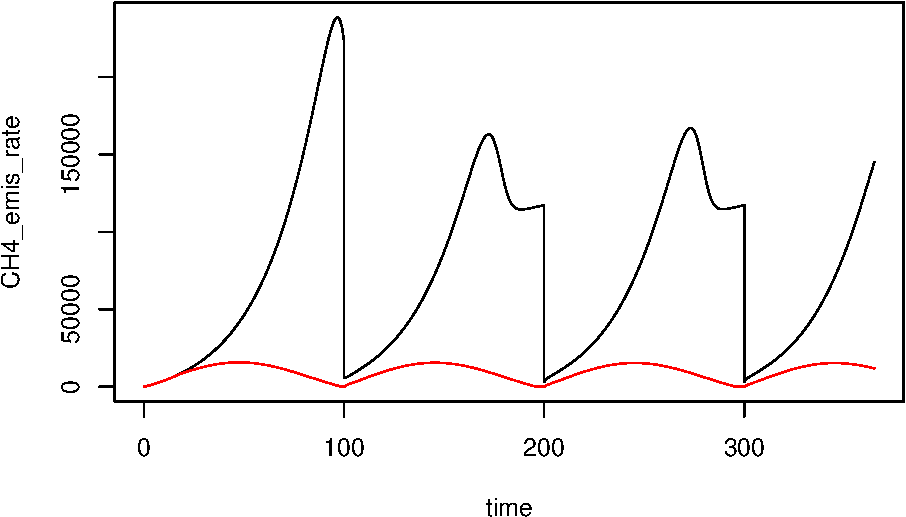
\includegraphics{simple_demo_files/figure-latex/unnamed-chunk-59-1.pdf}

\begin{Shaded}
\begin{Highlighting}[]
\FunctionTok{plot}\NormalTok{(CH4\_emis\_cum }\SpecialCharTok{\textasciitilde{}}\NormalTok{ time, }\AttributeTok{data =}\NormalTok{ out7, }\AttributeTok{type =} \StringTok{\textquotesingle{}l\textquotesingle{}}\NormalTok{)}
\FunctionTok{lines}\NormalTok{(CH4\_emis\_cum }\SpecialCharTok{\textasciitilde{}}\NormalTok{ time, }\AttributeTok{data =}\NormalTok{ out8, }\AttributeTok{col =} \StringTok{\textquotesingle{}red\textquotesingle{}}\NormalTok{)}
\end{Highlighting}
\end{Shaded}

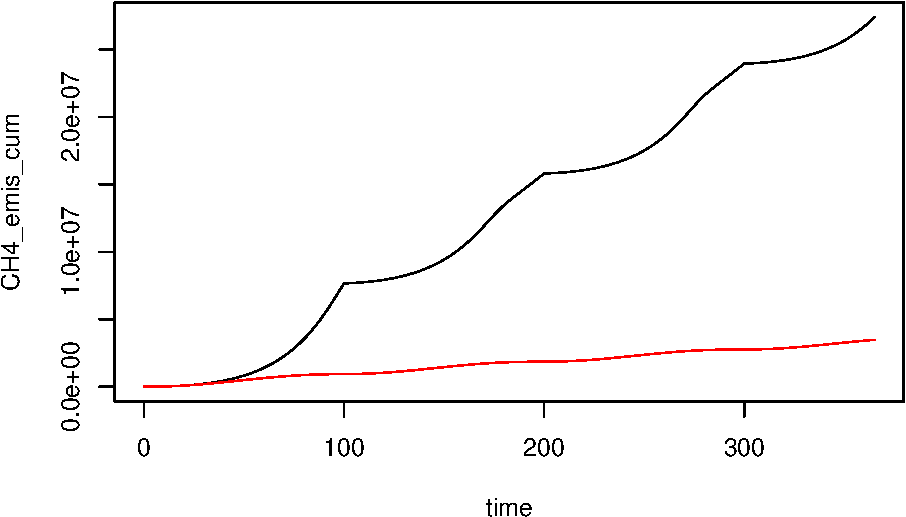
\includegraphics{simple_demo_files/figure-latex/unnamed-chunk-59-2.pdf}

\hypertarget{volatilization}{%
\section{9. Volatilization}\label{volatilization}}

Any chemical species can volatilize.

\begin{Shaded}
\begin{Highlighting}[]
\NormalTok{man\_pars9 }\OtherTok{\textless{}{-}} \FunctionTok{list}\NormalTok{(}\AttributeTok{comps =} \FunctionTok{c}\NormalTok{(}\StringTok{\textquotesingle{}H2S\textquotesingle{}}\NormalTok{, }\StringTok{\textquotesingle{}NH4p\textquotesingle{}}\NormalTok{),}
                 \AttributeTok{comp\_fresh =} \FunctionTok{c}\NormalTok{(}\AttributeTok{H2S =} \FloatTok{0.01}\NormalTok{, }\AttributeTok{NH4p =} \FloatTok{2.5}\NormalTok{), }
                 \AttributeTok{VFA\_fresh =} \FunctionTok{c}\NormalTok{(}\AttributeTok{CH3COOH =} \DecValTok{2}\NormalTok{),}
                 \AttributeTok{pH =} \DecValTok{7}\NormalTok{, }\AttributeTok{dens =} \DecValTok{1000}\NormalTok{)}
\end{Highlighting}
\end{Shaded}

We need to set mass transfer coefficient values (m/d) for any species
that volatilizes. These are overall (possibly two-film) values for in
liquid-phase units.

\begin{Shaded}
\begin{Highlighting}[]
\NormalTok{chem\_pars9 }\OtherTok{\textless{}{-}} \FunctionTok{list}\NormalTok{(}\AttributeTok{COD\_conv =} \FunctionTok{c}\NormalTok{(}\AttributeTok{CH4 =} \DecValTok{1}\SpecialCharTok{/}\FloatTok{0.2507}\NormalTok{),}
                   \AttributeTok{specs =} \FunctionTok{c}\NormalTok{(}\StringTok{\textquotesingle{}NH3\textquotesingle{}}\NormalTok{, }\StringTok{\textquotesingle{}HSm\textquotesingle{}}\NormalTok{, }\StringTok{\textquotesingle{}CH3COOm\textquotesingle{}}\NormalTok{),}
                   \AttributeTok{mspec =} \FunctionTok{c}\NormalTok{(}\AttributeTok{NH3 =} \StringTok{\textquotesingle{}NH4p\textquotesingle{}}\NormalTok{, }\AttributeTok{HSm =} \StringTok{\textquotesingle{}H2S\textquotesingle{}}\NormalTok{, }\AttributeTok{CH3COOm =} \StringTok{\textquotesingle{}CH3COOH\textquotesingle{}}\NormalTok{),}
                   \AttributeTok{lka =} \FunctionTok{c}\NormalTok{(}\AttributeTok{NH3 =} \StringTok{\textquotesingle{}{-} 0.09046 {-} 2729.31/temp\_K\textquotesingle{}}\NormalTok{, }
                           \AttributeTok{HSm =} \StringTok{\textquotesingle{}{-} 3448.7/temp\_K + 47.479 {-} 7.5227 * log(temp\_K)\textquotesingle{}}\NormalTok{,}
                           \AttributeTok{CH3COOm =} \StringTok{\textquotesingle{}{-}4.8288 + 21.42/temp\_K\textquotesingle{}}\NormalTok{),}
                   \AttributeTok{kl =} \FunctionTok{c}\NormalTok{(}\AttributeTok{NH3 =} \FloatTok{0.01}\NormalTok{, }\AttributeTok{H2S =} \FloatTok{0.01}\NormalTok{, }\AttributeTok{CH3COOH =} \FloatTok{0.01}\NormalTok{) }\SpecialCharTok{*} \DecValTok{86400}\NormalTok{)}
\end{Highlighting}
\end{Shaded}

\begin{Shaded}
\begin{Highlighting}[]
\NormalTok{devtools}\SpecialCharTok{::}\FunctionTok{load\_all}\NormalTok{()}
\end{Highlighting}
\end{Shaded}

\begin{verbatim}
## i Loading ABM
\end{verbatim}

\begin{Shaded}
\begin{Highlighting}[]
\NormalTok{out9a }\OtherTok{\textless{}{-}} \FunctionTok{abm}\NormalTok{(}\DecValTok{365}\NormalTok{,}
             \AttributeTok{mng\_pars =}\NormalTok{ mng\_pars,}
             \AttributeTok{man\_pars =}\NormalTok{ man\_pars9,}
             \AttributeTok{grp\_pars =}\NormalTok{ grp\_pars,}
             \AttributeTok{mic\_pars =}\NormalTok{ mic\_pars,}
             \AttributeTok{sub\_pars =}\NormalTok{ sub\_pars,}
             \AttributeTok{chem\_pars =}\NormalTok{ chem\_pars9,}
             \AttributeTok{inhib\_pars =}\NormalTok{ inhib\_pars}
\NormalTok{)}
\end{Highlighting}
\end{Shaded}

\begin{verbatim}
## Warning in expandPars(pars = pars, elnms = pars$grps, parnms = grp_par_nms):
## Size-variable parameter problem: Missing element(s) in kss.
\end{verbatim}

\begin{verbatim}
## Warning in checkCOD(dat = dat, grps = pars$grps, subs = pars$subs, COD_conv =
## pars$COD_conv, : COD balance is off by 2%
\end{verbatim}

The state variable vector and output data frame automatically expand for
the new values.

\begin{Shaded}
\begin{Highlighting}[]
\FunctionTok{head}\NormalTok{(out9a[, }\FunctionTok{grep}\NormalTok{(}\StringTok{\textquotesingle{}\_emis\textquotesingle{}}\NormalTok{, }\FunctionTok{names}\NormalTok{(out9a))])}
\end{Highlighting}
\end{Shaded}

\begin{verbatim}
##   CH4_emis_cum NH3_emis_cum H2S_emis_cum CH3COOH_emis_cum CH4_emis_rate
## 1       0.0000        0.000       0.0000            0.000      25.52844
## 2     161.8334      833.273      89.6908         1106.072     305.28189
## 3     622.3551     1661.702     171.2283         2484.484     620.73997
## 4    1412.0784     2489.451     252.7655         4130.203     962.63333
## 5    2554.8558     3316.914     334.3028         6036.464    1326.29785
## 6    4071.0922     4144.219     415.8401         8196.713    1709.25431
\end{verbatim}

\begin{Shaded}
\begin{Highlighting}[]
\FunctionTok{plot}\NormalTok{(NH4p\_conc }\SpecialCharTok{\textasciitilde{}}\NormalTok{ time, }\AttributeTok{data =}\NormalTok{ out8, }\AttributeTok{type =} \StringTok{\textquotesingle{}l\textquotesingle{}}\NormalTok{, }\AttributeTok{ylim =} \FunctionTok{c}\NormalTok{(}\DecValTok{0}\NormalTok{, }\DecValTok{3}\NormalTok{))}
\FunctionTok{lines}\NormalTok{(NH4p\_conc }\SpecialCharTok{\textasciitilde{}}\NormalTok{ time, }\AttributeTok{data =}\NormalTok{ out9a, }\AttributeTok{col =} \StringTok{\textquotesingle{}red\textquotesingle{}}\NormalTok{)}
\end{Highlighting}
\end{Shaded}

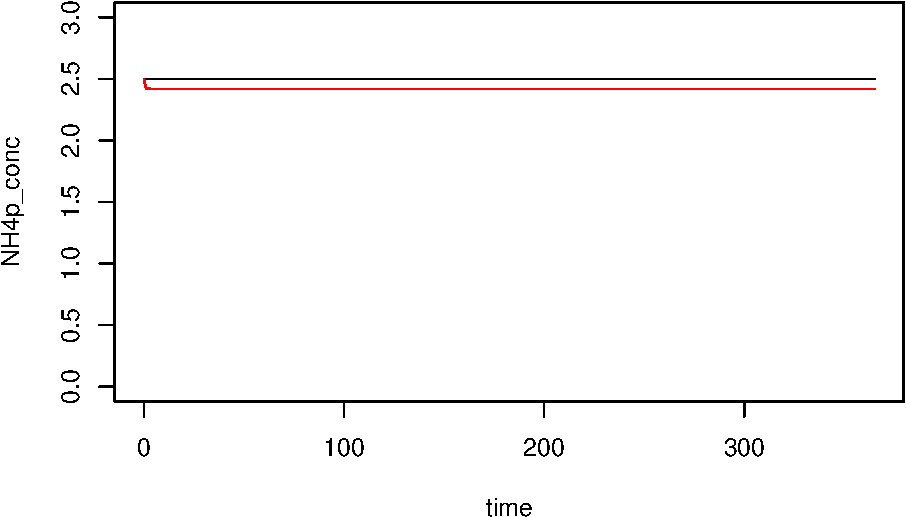
\includegraphics{simple_demo_files/figure-latex/unnamed-chunk-64-1.pdf}

\begin{Shaded}
\begin{Highlighting}[]
\FunctionTok{plot}\NormalTok{(NH4p }\SpecialCharTok{\textasciitilde{}}\NormalTok{ time, }\AttributeTok{data =}\NormalTok{ out8, }\AttributeTok{type =} \StringTok{\textquotesingle{}l\textquotesingle{}}\NormalTok{)}
\FunctionTok{lines}\NormalTok{(NH4p }\SpecialCharTok{\textasciitilde{}}\NormalTok{ time, }\AttributeTok{data =}\NormalTok{ out9a, }\AttributeTok{col =} \StringTok{\textquotesingle{}red\textquotesingle{}}\NormalTok{)}
\end{Highlighting}
\end{Shaded}

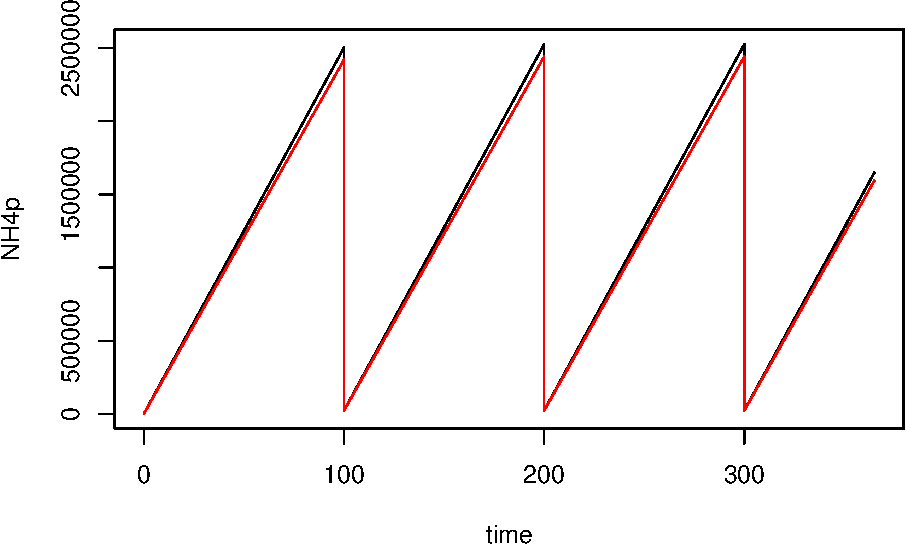
\includegraphics{simple_demo_files/figure-latex/unnamed-chunk-64-2.pdf}

\begin{Shaded}
\begin{Highlighting}[]
\FunctionTok{plot}\NormalTok{(NH3\_emis\_cum }\SpecialCharTok{\textasciitilde{}}\NormalTok{ time, }\AttributeTok{data =}\NormalTok{ out9a, }\AttributeTok{type =} \StringTok{\textquotesingle{}l\textquotesingle{}}\NormalTok{)}
\end{Highlighting}
\end{Shaded}

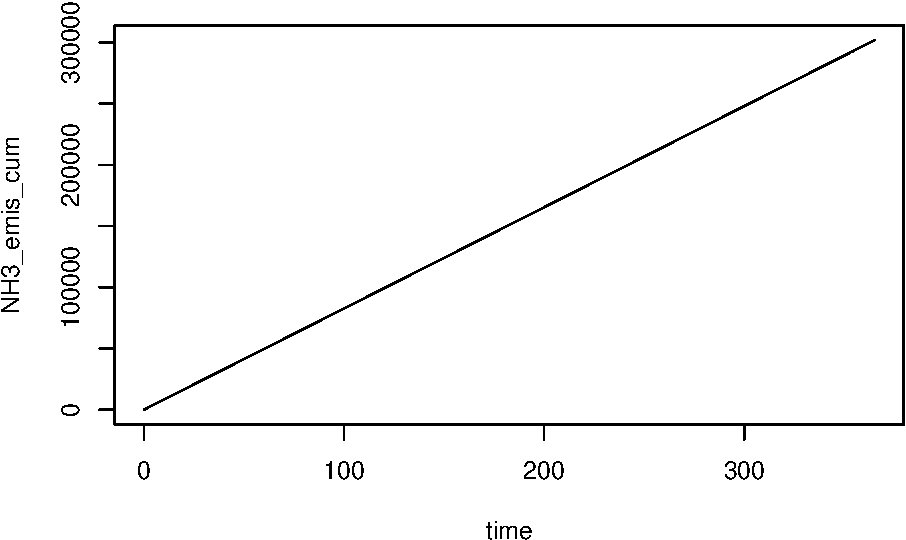
\includegraphics{simple_demo_files/figure-latex/unnamed-chunk-64-3.pdf}

\begin{Shaded}
\begin{Highlighting}[]
\FunctionTok{plot}\NormalTok{(H2S\_emis\_cum }\SpecialCharTok{\textasciitilde{}}\NormalTok{ time, }\AttributeTok{data =}\NormalTok{ out9a, }\AttributeTok{type =} \StringTok{\textquotesingle{}l\textquotesingle{}}\NormalTok{)}
\end{Highlighting}
\end{Shaded}

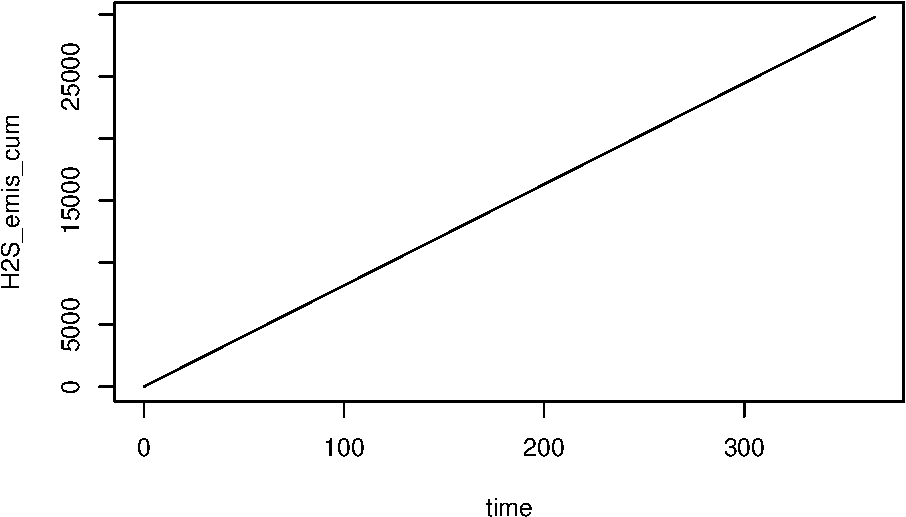
\includegraphics{simple_demo_files/figure-latex/unnamed-chunk-64-4.pdf}

\begin{Shaded}
\begin{Highlighting}[]
\FunctionTok{plot}\NormalTok{(CH3COOH\_emis\_cum }\SpecialCharTok{\textasciitilde{}}\NormalTok{ time, }\AttributeTok{data =}\NormalTok{ out9a, }\AttributeTok{type =} \StringTok{\textquotesingle{}l\textquotesingle{}}\NormalTok{)}
\end{Highlighting}
\end{Shaded}

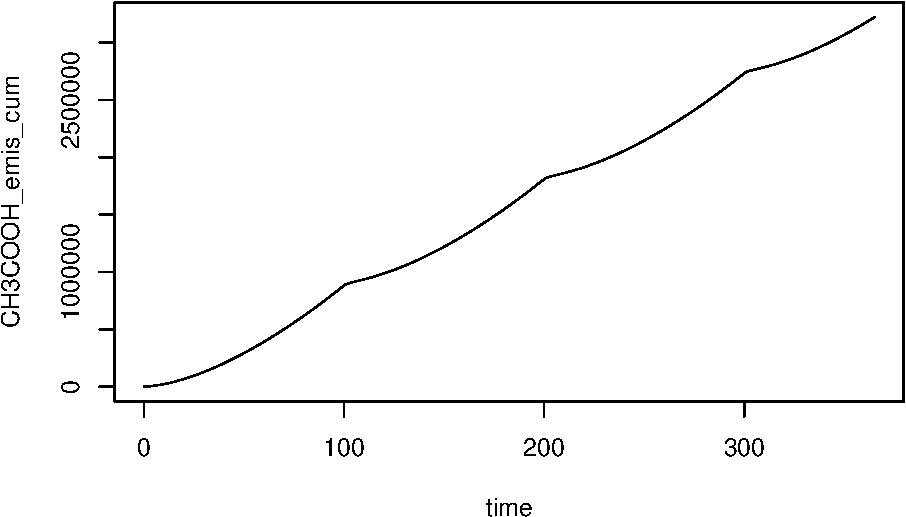
\includegraphics{simple_demo_files/figure-latex/unnamed-chunk-64-5.pdf}

Let's use a fixed slurry mass to exaggerate emission.

\begin{Shaded}
\begin{Highlighting}[]
\NormalTok{mng\_pars9b }\OtherTok{=} \FunctionTok{list}\NormalTok{(}\AttributeTok{slurry\_prod\_rate =} \DecValTok{0}\NormalTok{, }
                  \AttributeTok{slurry\_mass =} \FloatTok{1E6}\NormalTok{,     }
                  \AttributeTok{storage\_depth =} \DecValTok{2}\NormalTok{,     }
                  \AttributeTok{resid\_depth =} \FloatTok{0.1}\NormalTok{,      }
                  \AttributeTok{area =} \DecValTok{100}\NormalTok{,              }
                  \AttributeTok{empty\_int =} \DecValTok{100}\NormalTok{,          }
                  \AttributeTok{temp\_C =} \DecValTok{20}\NormalTok{,}
                  \AttributeTok{wash\_water =} \DecValTok{0}\NormalTok{,            }
                  \AttributeTok{wash\_int =} \ConstantTok{NA}\NormalTok{,}
                  \AttributeTok{rest\_d =} \DecValTok{0}\NormalTok{,}
                  \AttributeTok{resid\_enrich =} \DecValTok{1}\NormalTok{)}
\end{Highlighting}
\end{Shaded}

\begin{Shaded}
\begin{Highlighting}[]
\NormalTok{chem\_pars9b }\OtherTok{\textless{}{-}} \FunctionTok{list}\NormalTok{(}\AttributeTok{COD\_conv =} \FunctionTok{c}\NormalTok{(}\AttributeTok{CH4 =} \DecValTok{1}\SpecialCharTok{/}\FloatTok{0.2507}\NormalTok{, }\AttributeTok{xa =} \DecValTok{1}\SpecialCharTok{/}\FloatTok{0.7069561}\NormalTok{,}
                               \AttributeTok{VFA =} \DecValTok{1}\SpecialCharTok{/}\FloatTok{0.9383125}\NormalTok{, }\AttributeTok{S =} \DecValTok{1}\SpecialCharTok{/}\FloatTok{0.5015}\NormalTok{, }\AttributeTok{VS =} \DecValTok{1}\SpecialCharTok{/}\FloatTok{0.69}\NormalTok{, }
                               \AttributeTok{CO2\_aer =} \DecValTok{1}\SpecialCharTok{/}\FloatTok{0.436}\NormalTok{, }\AttributeTok{CO2\_sr =} \DecValTok{1}\SpecialCharTok{/}\FloatTok{1.2}\NormalTok{, }
                               \AttributeTok{C\_xa =} \DecValTok{1}\SpecialCharTok{/}\FloatTok{0.3753125}\NormalTok{),}
                   \AttributeTok{specs =} \FunctionTok{c}\NormalTok{(}\StringTok{\textquotesingle{}NH3\textquotesingle{}}\NormalTok{, }\StringTok{\textquotesingle{}HSm\textquotesingle{}}\NormalTok{, }\StringTok{\textquotesingle{}CH3COOm\textquotesingle{}}\NormalTok{),}
                   \AttributeTok{mspec =} \FunctionTok{c}\NormalTok{(}\AttributeTok{NH3 =} \StringTok{\textquotesingle{}NH4p\textquotesingle{}}\NormalTok{, }\AttributeTok{HSm =} \StringTok{\textquotesingle{}H2S\textquotesingle{}}\NormalTok{, }\AttributeTok{CH3COOm =} \StringTok{\textquotesingle{}CH3COOH\textquotesingle{}}\NormalTok{),}
                   \AttributeTok{lka =} \FunctionTok{c}\NormalTok{(}\AttributeTok{NH3 =} \StringTok{\textquotesingle{}{-} 0.09046 {-} 2729.31/temp\_K\textquotesingle{}}\NormalTok{, }
                           \AttributeTok{HSm =} \StringTok{\textquotesingle{}{-} 3448.7/temp\_K + 47.479 {-} 7.5227 * log(temp\_K)\textquotesingle{}}\NormalTok{,}
                           \AttributeTok{CH3COOm =} \StringTok{\textquotesingle{}{-}4.8288 + 21.42/temp\_K\textquotesingle{}}\NormalTok{),}
                   \AttributeTok{kl =} \FunctionTok{c}\NormalTok{(}\AttributeTok{NH3 =} \FloatTok{0.01}\NormalTok{, }\AttributeTok{H2S =} \FloatTok{0.01}\NormalTok{) }\SpecialCharTok{*} \DecValTok{86400}\NormalTok{)}
\end{Highlighting}
\end{Shaded}

\begin{Shaded}
\begin{Highlighting}[]
\NormalTok{devtools}\SpecialCharTok{::}\FunctionTok{load\_all}\NormalTok{()}
\end{Highlighting}
\end{Shaded}

\begin{verbatim}
## i Loading ABM
\end{verbatim}

\begin{Shaded}
\begin{Highlighting}[]
\NormalTok{out9b }\OtherTok{\textless{}{-}} \FunctionTok{abm}\NormalTok{(}\DecValTok{365}\NormalTok{,}
             \AttributeTok{mng\_pars =}\NormalTok{ mng\_pars9b,}
             \AttributeTok{man\_pars =}\NormalTok{ man\_pars9,}
             \AttributeTok{grp\_pars =}\NormalTok{ grp\_pars,}
             \AttributeTok{mic\_pars =}\NormalTok{ mic\_pars,}
             \AttributeTok{sub\_pars =}\NormalTok{ sub\_pars,}
             \AttributeTok{chem\_pars =}\NormalTok{ chem\_pars9b,}
             \AttributeTok{inhib\_pars =}\NormalTok{ inhib\_pars}
\NormalTok{)}
\end{Highlighting}
\end{Shaded}

\begin{verbatim}
## Warning in expandPars(pars = pars, elnms = pars$grps, parnms = grp_par_nms):
## Size-variable parameter problem: Missing element(s) in kss.
\end{verbatim}

\begin{verbatim}
## Warning in emptyStore(y, resid_mass = pars$resid_mass, resid_enrich =
## pars$resid_enrich): Emptying skipped.
## Warning in emptyStore(y, resid_mass = pars$resid_mass, resid_enrich =
## pars$resid_enrich): Emptying skipped.
\end{verbatim}

\begin{Shaded}
\begin{Highlighting}[]
\FunctionTok{plot}\NormalTok{(NH4p }\SpecialCharTok{\textasciitilde{}}\NormalTok{ time, }\AttributeTok{data =}\NormalTok{ out9b, }\AttributeTok{type =} \StringTok{\textquotesingle{}l\textquotesingle{}}\NormalTok{)}
\end{Highlighting}
\end{Shaded}

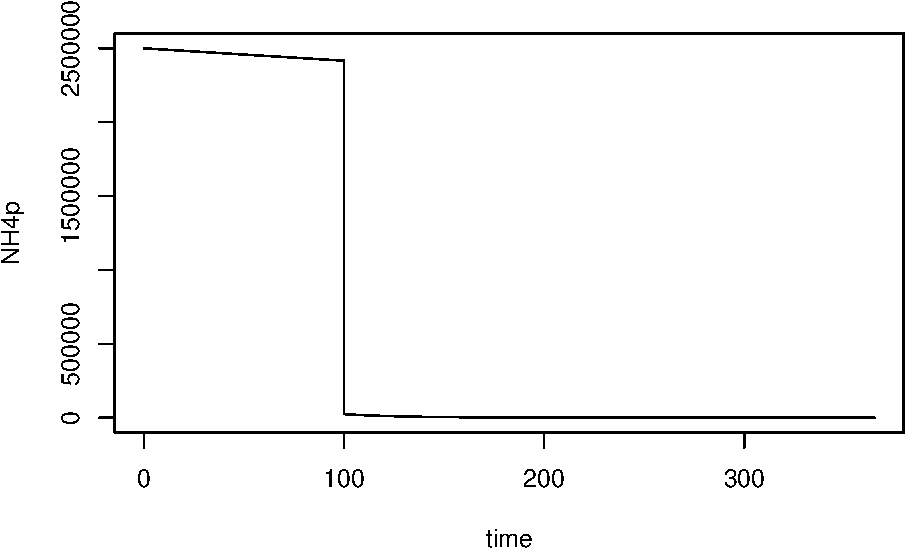
\includegraphics{simple_demo_files/figure-latex/unnamed-chunk-68-1.pdf}

\begin{Shaded}
\begin{Highlighting}[]
\FunctionTok{plot}\NormalTok{(NH4p\_conc }\SpecialCharTok{\textasciitilde{}}\NormalTok{ time, }\AttributeTok{data =}\NormalTok{ out9b, }\AttributeTok{type =} \StringTok{\textquotesingle{}l\textquotesingle{}}\NormalTok{)}
\end{Highlighting}
\end{Shaded}

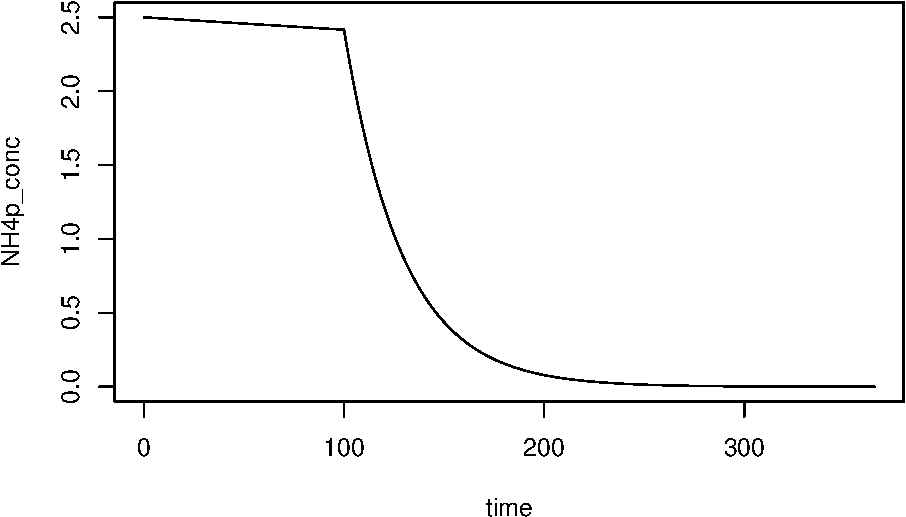
\includegraphics{simple_demo_files/figure-latex/unnamed-chunk-68-2.pdf}

\hypertarget{cod-balance}{%
\section{9. COD balance}\label{cod-balance}}

There is now a \texttt{checkCOD()} function that runs on \texttt{abm()}
results before returning them. For now the tolerance is fixed at 1\%.
Some of the examples above do not meet that criterion for some reason.
At least one shows a real problem that needs to be identified. For the
emission example above, the problem is that VFA is emitted but that loss
is not included in the balance check (this might have been fixed). I
need to decide about how to pass that COD information. We can make it
worse by pretending the the charged form can volatilize (\texttt{VFA}
changed to \texttt{CH3COOm} below).

\begin{Shaded}
\begin{Highlighting}[]
\NormalTok{chem\_pars10 }\OtherTok{\textless{}{-}} \FunctionTok{list}\NormalTok{(}\AttributeTok{COD\_conv =} \FunctionTok{c}\NormalTok{(}\AttributeTok{CH4 =} \DecValTok{1}\SpecialCharTok{/}\FloatTok{0.2507}\NormalTok{, }\AttributeTok{xa =} \DecValTok{1}\SpecialCharTok{/}\FloatTok{0.7069561}\NormalTok{,}
                               \AttributeTok{VFA =} \DecValTok{1}\SpecialCharTok{/}\FloatTok{0.9383125}\NormalTok{, }\AttributeTok{S =} \DecValTok{1}\SpecialCharTok{/}\FloatTok{0.5015}\NormalTok{, }\AttributeTok{VS =} \DecValTok{1}\SpecialCharTok{/}\FloatTok{0.69}\NormalTok{, }
                               \AttributeTok{CO2\_aer =} \DecValTok{1}\SpecialCharTok{/}\FloatTok{0.436}\NormalTok{, }\AttributeTok{CO2\_sr =} \DecValTok{1}\SpecialCharTok{/}\FloatTok{1.2}\NormalTok{, }
                               \AttributeTok{C\_xa =} \DecValTok{1}\SpecialCharTok{/}\FloatTok{0.3753125}\NormalTok{),}
                   \AttributeTok{specs =} \FunctionTok{c}\NormalTok{(}\StringTok{\textquotesingle{}NH3\textquotesingle{}}\NormalTok{, }\StringTok{\textquotesingle{}HSm\textquotesingle{}}\NormalTok{, }\StringTok{\textquotesingle{}CH3COOm\textquotesingle{}}\NormalTok{),}
                   \AttributeTok{mspec =} \FunctionTok{c}\NormalTok{(}\AttributeTok{NH3 =} \StringTok{\textquotesingle{}NH4p\textquotesingle{}}\NormalTok{, }\AttributeTok{HSm =} \StringTok{\textquotesingle{}H2S\textquotesingle{}}\NormalTok{, }\AttributeTok{CH3COOm =} \StringTok{\textquotesingle{}CH3COOH\textquotesingle{}}\NormalTok{),}
                   \AttributeTok{lka =} \FunctionTok{c}\NormalTok{(}\AttributeTok{NH3 =} \StringTok{\textquotesingle{}{-} 0.09046 {-} 2729.31/temp\_K\textquotesingle{}}\NormalTok{, }
                           \AttributeTok{HSm =} \StringTok{\textquotesingle{}{-} 3448.7/temp\_K + 47.479 {-} 7.5227 * log(temp\_K)\textquotesingle{}}\NormalTok{,}
                           \AttributeTok{CH3COOm =} \StringTok{\textquotesingle{}{-}4.8288 + 21.42/temp\_K\textquotesingle{}}\NormalTok{),}
                   \AttributeTok{kl =} \FunctionTok{c}\NormalTok{(}\AttributeTok{NH3 =} \FloatTok{0.01}\NormalTok{, }\AttributeTok{H2S =} \FloatTok{0.01}\NormalTok{, }\AttributeTok{CH3COOm =} \FloatTok{0.01}\NormalTok{) }\SpecialCharTok{*} \DecValTok{86400}\NormalTok{)}
\end{Highlighting}
\end{Shaded}

\begin{Shaded}
\begin{Highlighting}[]
\NormalTok{out10 }\OtherTok{\textless{}{-}} \FunctionTok{abm}\NormalTok{(}\DecValTok{365}\NormalTok{,}
            \AttributeTok{mng\_pars =}\NormalTok{ mng\_pars,}
            \AttributeTok{man\_pars =}\NormalTok{ man\_pars9,}
            \AttributeTok{grp\_pars =}\NormalTok{ grp\_pars,}
            \AttributeTok{mic\_pars =}\NormalTok{ mic\_pars,}
            \AttributeTok{sub\_pars =}\NormalTok{ sub\_pars,}
            \AttributeTok{chem\_pars =}\NormalTok{ chem\_pars10,}
            \AttributeTok{inhib\_pars =}\NormalTok{ inhib\_pars}
\NormalTok{)}
\end{Highlighting}
\end{Shaded}

\begin{verbatim}
## Warning in expandPars(pars = pars, elnms = pars$grps, parnms = grp_par_nms):
## Size-variable parameter problem: Missing element(s) in kss.
\end{verbatim}

\begin{verbatim}
## Warning in checkCOD(dat = dat, grps = pars$grps, subs = pars$subs, COD_conv =
## pars$COD_conv, : COD balance is off by 36%
\end{verbatim}

\hypertarget{stoichiometry-and-nitrogen-mineralization}{%
\section{10. Stoichiometry and nitrogen
mineralization}\label{stoichiometry-and-nitrogen-mineralization}}

Now substrates can produce any amount of arbitrary components (defined
in \texttt{man\_pars}, possibly volatilized, possibly involved in
speciation in inhibition) through hydrolysis and fermentation to VFA.

\begin{Shaded}
\begin{Highlighting}[]
\NormalTok{man\_pars10 }\OtherTok{\textless{}{-}} \FunctionTok{list}\NormalTok{(}\AttributeTok{comps =} \FunctionTok{c}\NormalTok{(}\StringTok{\textquotesingle{}H2S\textquotesingle{}}\NormalTok{, }\StringTok{\textquotesingle{}SO4m2\textquotesingle{}}\NormalTok{, }\StringTok{\textquotesingle{}NH4p\textquotesingle{}}\NormalTok{),}
                   \AttributeTok{comp\_fresh =} \FunctionTok{c}\NormalTok{(}\AttributeTok{H2S =} \FloatTok{0.01}\NormalTok{, }\AttributeTok{SO4m2 =} \FloatTok{0.2}\NormalTok{, }\AttributeTok{NH4p =} \FloatTok{2.5}\NormalTok{), }
                   \AttributeTok{VFA\_fresh =} \FunctionTok{c}\NormalTok{(}\AttributeTok{CH3COOH =} \DecValTok{2}\NormalTok{),}
                   \AttributeTok{pH =} \DecValTok{7}\NormalTok{, }\AttributeTok{dens =} \DecValTok{1000}\NormalTok{)}
\end{Highlighting}
\end{Shaded}

(Hmm, should \texttt{comps} be moved to \texttt{chem\_pars}?)

Here we'll have 4 substrates. But substrates need not actually produce
VFA anymore.

\begin{Shaded}
\begin{Highlighting}[]
\NormalTok{sub\_pars10 }\OtherTok{\textless{}{-}} \FunctionTok{list}\NormalTok{(}\AttributeTok{subs =} \FunctionTok{c}\NormalTok{(}\StringTok{\textquotesingle{}cellulose\textquotesingle{}}\NormalTok{, }\StringTok{\textquotesingle{}protein\textquotesingle{}}\NormalTok{, }\StringTok{\textquotesingle{}lipids\textquotesingle{}}\NormalTok{, }\StringTok{\textquotesingle{}urea\textquotesingle{}}\NormalTok{),}
                   \AttributeTok{T\_opt\_hyd =} \FunctionTok{c}\NormalTok{(}\AttributeTok{all =} \DecValTok{60}\NormalTok{),}
                   \AttributeTok{T\_min\_hyd =} \FunctionTok{c}\NormalTok{(}\AttributeTok{all =} \DecValTok{0}\NormalTok{),}
                   \AttributeTok{T\_max\_hyd =} \FunctionTok{c}\NormalTok{(}\AttributeTok{all =} \DecValTok{90}\NormalTok{),}
                   \AttributeTok{hydrol\_opt =} \FunctionTok{c}\NormalTok{(}\AttributeTok{lipids =} \FloatTok{0.1}\NormalTok{, }\AttributeTok{protein =} \FloatTok{0.01}\NormalTok{, }\AttributeTok{cellulose =} \FloatTok{0.05}\NormalTok{, }\AttributeTok{urea =} \DecValTok{1}\NormalTok{),}
                   \AttributeTok{sub\_fresh =} \FunctionTok{c}\NormalTok{(}\AttributeTok{lipids =} \DecValTok{3}\NormalTok{, }\AttributeTok{protein =} \DecValTok{20}\NormalTok{, }\AttributeTok{cellulose =} \DecValTok{35}\NormalTok{, }\AttributeTok{urea =} \DecValTok{10}\NormalTok{),}
                   \AttributeTok{sub\_init =} \FunctionTok{c}\NormalTok{(}\AttributeTok{lipids =} \DecValTok{3}\NormalTok{, }\AttributeTok{protein =} \DecValTok{20}\NormalTok{, }\AttributeTok{cellulose =} \DecValTok{35}\NormalTok{, }\AttributeTok{urea =} \DecValTok{10}\NormalTok{))}
\end{Highlighting}
\end{Shaded}

Production of any component is set in the \texttt{stoich} element of the
\texttt{chem\_pars} argument.

\begin{Shaded}
\begin{Highlighting}[]
\NormalTok{smat }\OtherTok{\textless{}{-}} \FunctionTok{matrix}\NormalTok{(}\FunctionTok{c}\NormalTok{(}\DecValTok{0}\NormalTok{, }\FloatTok{0.2}\NormalTok{,  }\DecValTok{0}\NormalTok{, }\FloatTok{0.2}\NormalTok{,}
                 \DecValTok{0}\NormalTok{, }\FloatTok{0.01}\NormalTok{, }\DecValTok{0}\NormalTok{, }\DecValTok{0}\NormalTok{,}
                 \DecValTok{1}\NormalTok{, }\DecValTok{1}\NormalTok{,    }\DecValTok{1}\NormalTok{, }\DecValTok{0}\NormalTok{),}
               \AttributeTok{nrow =} \DecValTok{3}\NormalTok{,}
               \AttributeTok{byrow =} \ConstantTok{TRUE}\NormalTok{,}
               \AttributeTok{dimnames =} \FunctionTok{list}\NormalTok{(}
                 \FunctionTok{c}\NormalTok{(}\StringTok{\textquotesingle{}NH4p\textquotesingle{}}\NormalTok{, }\StringTok{\textquotesingle{}H2S\textquotesingle{}}\NormalTok{, }\StringTok{\textquotesingle{}CH3COOH\textquotesingle{}}\NormalTok{),}
                 \FunctionTok{c}\NormalTok{(}\StringTok{\textquotesingle{}cellulose\textquotesingle{}}\NormalTok{, }\StringTok{\textquotesingle{}protein\textquotesingle{}}\NormalTok{, }\StringTok{\textquotesingle{}lipids\textquotesingle{}}\NormalTok{, }\StringTok{\textquotesingle{}urea\textquotesingle{}}\NormalTok{)))}

\NormalTok{smat}
\end{Highlighting}
\end{Shaded}

\begin{verbatim}
##         cellulose protein lipids urea
## NH4p            0    0.20      0  0.2
## H2S             0    0.01      0  0.0
## CH3COOH         1    1.00      1  0.0
\end{verbatim}

Substrate and other component quantities are

\begin{enumerate}
\def\labelenumi{\arabic{enumi}.}
\tightlist
\item
  COD mass, or if COD = 0,
\item
  N mass, or if N = 0,
\item
  C mass, or if C = 0,
\item
  S mass, or if S = 0,
\item
  total mass
\end{enumerate}

So the \texttt{CH3COOH} row should only have 1 or 0.

The \texttt{stoich} matrix can be calculated from substrate chemical
formulas--see next example.

\begin{Shaded}
\begin{Highlighting}[]
\NormalTok{chem\_pars10 }\OtherTok{\textless{}{-}} \FunctionTok{list}\NormalTok{(}\AttributeTok{COD\_conv =} \FunctionTok{c}\NormalTok{(}\AttributeTok{CH4 =} \DecValTok{1}\SpecialCharTok{/}\FloatTok{0.2507}\NormalTok{, }\AttributeTok{xa =} \DecValTok{1}\SpecialCharTok{/}\FloatTok{0.7069561}\NormalTok{,}
                               \AttributeTok{VFA =} \DecValTok{1}\SpecialCharTok{/}\FloatTok{0.9383125}\NormalTok{, }\AttributeTok{S =} \DecValTok{1}\SpecialCharTok{/}\FloatTok{0.5015}\NormalTok{, }\AttributeTok{VS =} \DecValTok{1}\SpecialCharTok{/}\FloatTok{0.69}\NormalTok{, }
                               \AttributeTok{CO2\_aer =} \DecValTok{1}\SpecialCharTok{/}\FloatTok{0.436}\NormalTok{, }\AttributeTok{CO2\_sr =} \DecValTok{1}\SpecialCharTok{/}\FloatTok{1.2}\NormalTok{, }
                               \AttributeTok{C\_xa =} \DecValTok{1}\SpecialCharTok{/}\FloatTok{0.3753125}\NormalTok{),}
                    \AttributeTok{specs =} \FunctionTok{c}\NormalTok{(}\StringTok{\textquotesingle{}NH3\textquotesingle{}}\NormalTok{, }\StringTok{\textquotesingle{}HSm\textquotesingle{}}\NormalTok{, }\StringTok{\textquotesingle{}CH3COOm\textquotesingle{}}\NormalTok{),}
                    \AttributeTok{mspec =} \FunctionTok{c}\NormalTok{(}\AttributeTok{NH3 =} \StringTok{\textquotesingle{}NH4p\textquotesingle{}}\NormalTok{, }\AttributeTok{HSm =} \StringTok{\textquotesingle{}H2S\textquotesingle{}}\NormalTok{, }\AttributeTok{CH3COOm =} \StringTok{\textquotesingle{}CH3COOH\textquotesingle{}}\NormalTok{),}
                    \AttributeTok{stoich =}\NormalTok{ smat)}
\end{Highlighting}
\end{Shaded}

\begin{Shaded}
\begin{Highlighting}[]
\NormalTok{devtools}\SpecialCharTok{::}\FunctionTok{load\_all}\NormalTok{()}
\end{Highlighting}
\end{Shaded}

\begin{verbatim}
## i Loading ABM
\end{verbatim}

\begin{Shaded}
\begin{Highlighting}[]
\NormalTok{out10 }\OtherTok{\textless{}{-}} \FunctionTok{abm}\NormalTok{(}\DecValTok{365}\NormalTok{,}
            \AttributeTok{mng\_pars =}\NormalTok{ mng\_pars,}
            \AttributeTok{man\_pars =}\NormalTok{ man\_pars10,}
            \AttributeTok{grp\_pars =}\NormalTok{ grp\_pars,}
            \AttributeTok{mic\_pars =}\NormalTok{ mic\_pars,}
            \AttributeTok{sub\_pars =}\NormalTok{ sub\_pars10,}
            \AttributeTok{chem\_pars =}\NormalTok{ chem\_pars10)}
\end{Highlighting}
\end{Shaded}

\begin{verbatim}
## Warning in expandPars(pars = pars, elnms = pars$grps, parnms = grp_par_nms):
## Size-variable parameter problem: Missing element(s) in kss.
\end{verbatim}

\begin{verbatim}
## Warning in checkCOD(dat = dat, grps = pars$grps, subs = pars$subs, COD_conv =
## pars$COD_conv, : COD balance is off by 1.2%
\end{verbatim}

\begin{Shaded}
\begin{Highlighting}[]
\FunctionTok{plot}\NormalTok{(CH3COOH\_conc }\SpecialCharTok{\textasciitilde{}}\NormalTok{ time, }\AttributeTok{data =}\NormalTok{ out10, }\AttributeTok{type =} \StringTok{\textquotesingle{}l\textquotesingle{}}\NormalTok{)}
\end{Highlighting}
\end{Shaded}

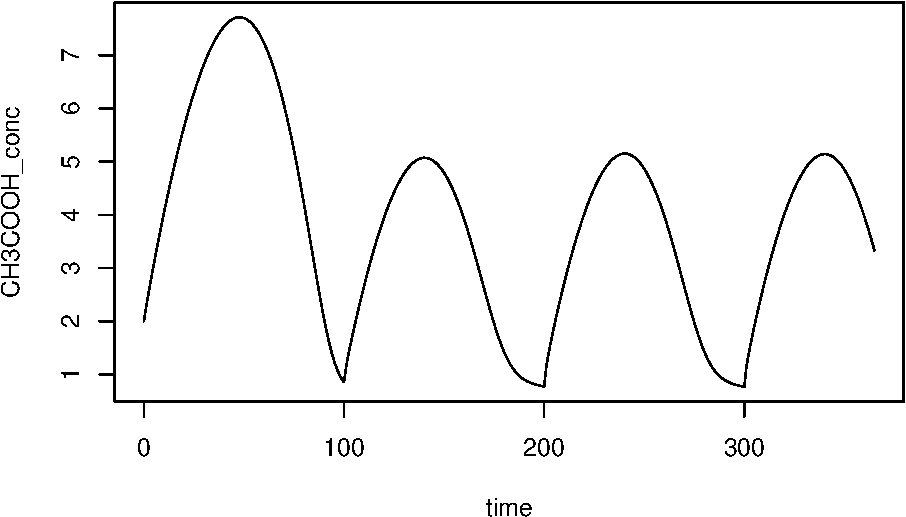
\includegraphics{simple_demo_files/figure-latex/unnamed-chunk-76-1.pdf}

\begin{Shaded}
\begin{Highlighting}[]
\FunctionTok{plot}\NormalTok{(urea\_conc }\SpecialCharTok{\textasciitilde{}}\NormalTok{ time, }\AttributeTok{data =}\NormalTok{ out10, }\AttributeTok{type =} \StringTok{\textquotesingle{}l\textquotesingle{}}\NormalTok{, }\AttributeTok{ylab =} \StringTok{\textquotesingle{}Urea or TAN (g/kg)\textquotesingle{}}\NormalTok{)}
\FunctionTok{lines}\NormalTok{(NH4p\_conc }\SpecialCharTok{\textasciitilde{}}\NormalTok{ time, }\AttributeTok{data =}\NormalTok{ out10, }\AttributeTok{col =} \StringTok{\textquotesingle{}blue\textquotesingle{}}\NormalTok{)}
\end{Highlighting}
\end{Shaded}

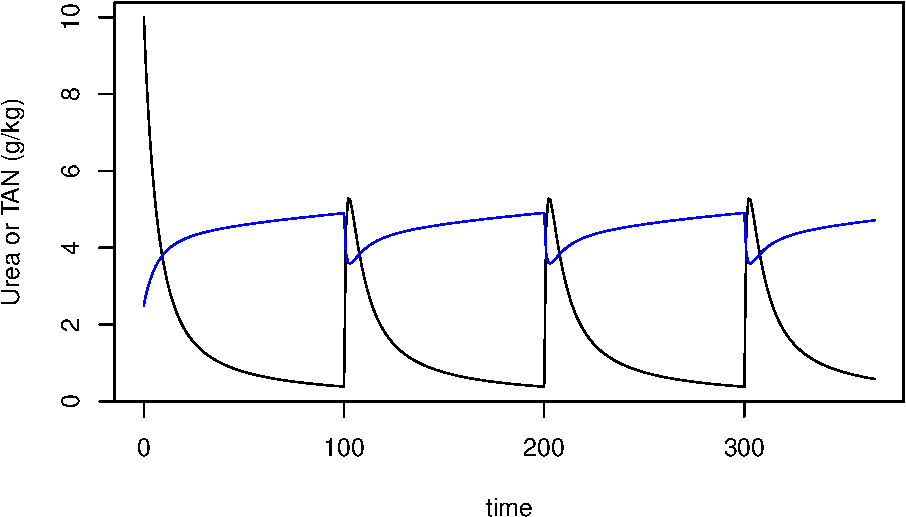
\includegraphics{simple_demo_files/figure-latex/unnamed-chunk-76-2.pdf}

It might make more sense to have \texttt{stoich} calculated internally.
For this, substrate formulas must be provided.

\begin{Shaded}
\begin{Highlighting}[]
\NormalTok{sub\_pars10b }\OtherTok{\textless{}{-}} \FunctionTok{list}\NormalTok{(}\AttributeTok{subs =} \FunctionTok{c}\NormalTok{(}\StringTok{\textquotesingle{}cellulose\textquotesingle{}}\NormalTok{, }\StringTok{\textquotesingle{}protein\textquotesingle{}}\NormalTok{, }\StringTok{\textquotesingle{}lipids\textquotesingle{}}\NormalTok{, }\StringTok{\textquotesingle{}urea\textquotesingle{}}\NormalTok{),}
                    \AttributeTok{forms =} \FunctionTok{c}\NormalTok{(}\AttributeTok{cellulose =} \StringTok{\textquotesingle{}C6H10O5\textquotesingle{}}\NormalTok{, }\AttributeTok{protein =} \StringTok{\textquotesingle{}C4 H6.1 O1.2 N\textquotesingle{}}\NormalTok{,}
                              \AttributeTok{lipids =} \StringTok{\textquotesingle{}C57 H104 O6\textquotesingle{}}\NormalTok{, }\AttributeTok{urea =} \StringTok{\textquotesingle{}CO(NH2)2\textquotesingle{}}\NormalTok{),}
                    \AttributeTok{T\_opt\_hyd =} \FunctionTok{c}\NormalTok{(}\AttributeTok{all =} \DecValTok{60}\NormalTok{),}
                    \AttributeTok{T\_min\_hyd =} \FunctionTok{c}\NormalTok{(}\AttributeTok{all =} \DecValTok{0}\NormalTok{),}
                    \AttributeTok{T\_max\_hyd =} \FunctionTok{c}\NormalTok{(}\AttributeTok{all =} \DecValTok{90}\NormalTok{),}
                    \AttributeTok{hydrol\_opt =} \FunctionTok{c}\NormalTok{(}\AttributeTok{lipids =} \FloatTok{0.1}\NormalTok{, }\AttributeTok{protein =} \FloatTok{0.01}\NormalTok{, }\AttributeTok{cellulose =} \FloatTok{0.05}\NormalTok{, }\AttributeTok{urea =} \DecValTok{1}\NormalTok{),}
                    \AttributeTok{sub\_fresh =} \FunctionTok{c}\NormalTok{(}\AttributeTok{lipids =} \DecValTok{3}\NormalTok{, }\AttributeTok{protein =} \DecValTok{20}\NormalTok{, }\AttributeTok{cellulose =} \DecValTok{35}\NormalTok{, }\AttributeTok{urea =} \DecValTok{10}\NormalTok{),}
                    \AttributeTok{sub\_init =} \FunctionTok{c}\NormalTok{(}\AttributeTok{lipids =} \DecValTok{3}\NormalTok{, }\AttributeTok{protein =} \DecValTok{20}\NormalTok{, }\AttributeTok{cellulose =} \DecValTok{35}\NormalTok{, }\AttributeTok{urea =} \DecValTok{10}\NormalTok{))}
\end{Highlighting}
\end{Shaded}

Internally, the \texttt{getStoich()} function is used, which in turn
calls \texttt{predFerm()}. Among these substrates, cellulose produces no
CO2 from fermentation, protein and lipids \emph{consume} CO2 (they are
highly reduced), and urea is a special case with no COD. So it produces
no VFAs.

\begin{Shaded}
\begin{Highlighting}[]
\FunctionTok{predFerm}\NormalTok{(sub\_pars10b}\SpecialCharTok{$}\NormalTok{forms[}\DecValTok{1}\NormalTok{])}
\end{Highlighting}
\end{Shaded}

\begin{verbatim}
##     H2O CH3COOH 
##      -1       3
\end{verbatim}

\begin{Shaded}
\begin{Highlighting}[]
\FunctionTok{predFerm}\NormalTok{(sub\_pars10b}\SpecialCharTok{$}\NormalTok{forms[}\DecValTok{2}\NormalTok{])}
\end{Highlighting}
\end{Shaded}

\begin{verbatim}
##     H2O     CO2 CH3COOH     NH3 
## -2.6250 -0.1750  2.0875  1.0000
\end{verbatim}

\begin{Shaded}
\begin{Highlighting}[]
\FunctionTok{predFerm}\NormalTok{(sub\_pars10b}\SpecialCharTok{$}\NormalTok{forms[}\DecValTok{3}\NormalTok{])}
\end{Highlighting}
\end{Shaded}

\begin{verbatim}
##     H2O     CO2 CH3COOH 
##     -28     -23      40
\end{verbatim}

\begin{Shaded}
\begin{Highlighting}[]
\FunctionTok{predFerm}\NormalTok{(sub\_pars10b}\SpecialCharTok{$}\NormalTok{forms[}\DecValTok{4}\NormalTok{])}
\end{Highlighting}
\end{Shaded}

\begin{verbatim}
##     CO2     NH3      H.     H2O CH3COOH      H2 
##       1       2       0      -1       0       0
\end{verbatim}

Internally, the stiochiometric coefficients are changed to the same
units given above (COD, N, C, S, or total mass). Now we must have CO2 as
a component, because it will be produced.

\begin{Shaded}
\begin{Highlighting}[]
\NormalTok{man\_pars10b }\OtherTok{\textless{}{-}} \FunctionTok{list}\NormalTok{(}\AttributeTok{comps =} \FunctionTok{c}\NormalTok{(}\StringTok{\textquotesingle{}H2S\textquotesingle{}}\NormalTok{, }\StringTok{\textquotesingle{}SO4m2\textquotesingle{}}\NormalTok{, }\StringTok{\textquotesingle{}NH4p\textquotesingle{}}\NormalTok{, }\StringTok{\textquotesingle{}CO2\textquotesingle{}}\NormalTok{),}
                   \AttributeTok{comp\_fresh =} \FunctionTok{c}\NormalTok{(}\AttributeTok{H2S =} \FloatTok{0.01}\NormalTok{, }\AttributeTok{SO4m2 =} \FloatTok{0.2}\NormalTok{, }\AttributeTok{NH4p =} \FloatTok{2.5}\NormalTok{, }\AttributeTok{CO2 =} \DecValTok{1}\NormalTok{), }
                   \AttributeTok{VFA\_fresh =} \FunctionTok{c}\NormalTok{(}\AttributeTok{CH3COOH =} \DecValTok{2}\NormalTok{),}
                   \AttributeTok{pH =} \DecValTok{7}\NormalTok{, }\AttributeTok{dens =} \DecValTok{1000}\NormalTok{)}
\end{Highlighting}
\end{Shaded}

We don't actually need the species included above. But because of a bit
of a programming quirk, we need to provide the master species for NH3.

\begin{Shaded}
\begin{Highlighting}[]
\NormalTok{chem\_pars10b }\OtherTok{\textless{}{-}} \FunctionTok{list}\NormalTok{(}\AttributeTok{COD\_conv =} \FunctionTok{c}\NormalTok{(}\AttributeTok{CH4 =} \DecValTok{1}\SpecialCharTok{/}\FloatTok{0.2507}\NormalTok{),}
                    \AttributeTok{specs =} \FunctionTok{c}\NormalTok{(}\StringTok{\textquotesingle{}NH3\textquotesingle{}}\NormalTok{),}
                    \AttributeTok{mspec =} \FunctionTok{c}\NormalTok{(}\AttributeTok{NH3 =} \StringTok{\textquotesingle{}NH4p\textquotesingle{}}\NormalTok{),}
                    \AttributeTok{stoich =} \StringTok{\textquotesingle{}calc\textquotesingle{}}\NormalTok{)}
\end{Highlighting}
\end{Shaded}

\begin{Shaded}
\begin{Highlighting}[]
\NormalTok{devtools}\SpecialCharTok{::}\FunctionTok{load\_all}\NormalTok{()}
\end{Highlighting}
\end{Shaded}

\begin{verbatim}
## i Loading ABM
\end{verbatim}

\begin{Shaded}
\begin{Highlighting}[]
\NormalTok{out10b }\OtherTok{\textless{}{-}} \FunctionTok{abm}\NormalTok{(}\DecValTok{365}\NormalTok{,}
            \AttributeTok{mng\_pars =}\NormalTok{ mng\_pars,}
            \AttributeTok{man\_pars =}\NormalTok{ man\_pars10b,}
            \AttributeTok{grp\_pars =}\NormalTok{ grp\_pars,}
            \AttributeTok{mic\_pars =}\NormalTok{ mic\_pars,}
            \AttributeTok{sub\_pars =}\NormalTok{ sub\_pars10b,}
            \AttributeTok{chem\_pars =}\NormalTok{ chem\_pars10b)}
\end{Highlighting}
\end{Shaded}

\begin{verbatim}
## Warning in expandPars(pars = pars, elnms = pars$grps, parnms = grp_par_nms):
## Size-variable parameter problem: Missing element(s) in kss.
\end{verbatim}

\begin{verbatim}
## Warning in checkCOD(dat = dat, grps = pars$grps, subs = pars$subs, COD_conv =
## pars$COD_conv, : COD balance is off by 1.2%
\end{verbatim}

\begin{Shaded}
\begin{Highlighting}[]
\FunctionTok{plot}\NormalTok{(CH3COOH\_conc }\SpecialCharTok{\textasciitilde{}}\NormalTok{ time, }\AttributeTok{data =}\NormalTok{ out10b, }\AttributeTok{type =} \StringTok{\textquotesingle{}l\textquotesingle{}}\NormalTok{)}
\end{Highlighting}
\end{Shaded}

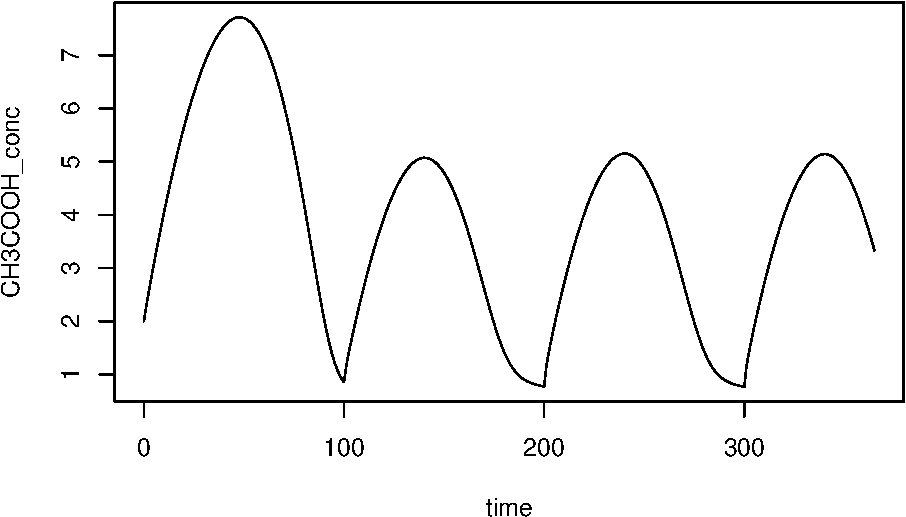
\includegraphics{simple_demo_files/figure-latex/unnamed-chunk-82-1.pdf}

\begin{Shaded}
\begin{Highlighting}[]
\FunctionTok{plot}\NormalTok{(urea\_conc }\SpecialCharTok{\textasciitilde{}}\NormalTok{ time, }\AttributeTok{data =}\NormalTok{ out10b, }\AttributeTok{type =} \StringTok{\textquotesingle{}l\textquotesingle{}}\NormalTok{, }\AttributeTok{ylab =} \StringTok{\textquotesingle{}Urea or TAN (g/kg)\textquotesingle{}}\NormalTok{)}
\FunctionTok{lines}\NormalTok{(NH4p\_conc }\SpecialCharTok{\textasciitilde{}}\NormalTok{ time, }\AttributeTok{data =}\NormalTok{ out10b, }\AttributeTok{col =} \StringTok{\textquotesingle{}blue\textquotesingle{}}\NormalTok{)}
\end{Highlighting}
\end{Shaded}

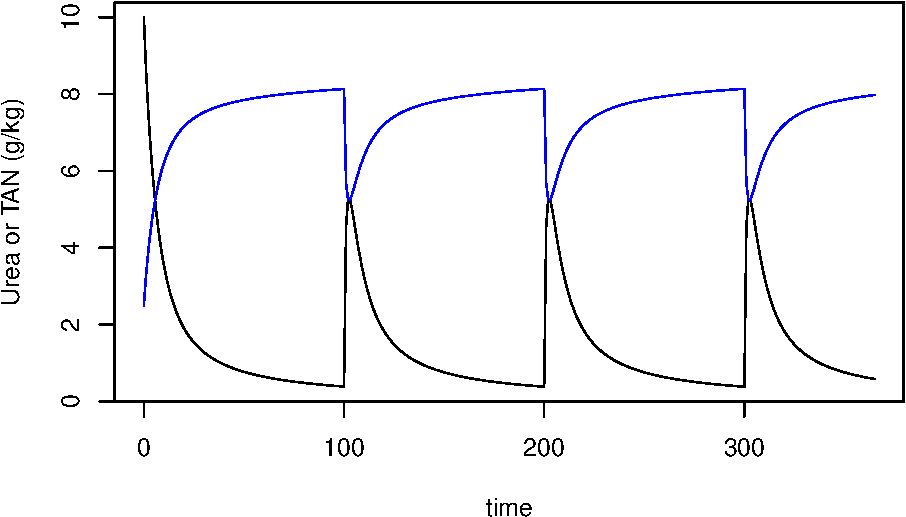
\includegraphics{simple_demo_files/figure-latex/unnamed-chunk-82-2.pdf}

Now we also have dissolved CO2 (really TIC) concentration. Only there is
no emission, so it does not mean much.

\begin{Shaded}
\begin{Highlighting}[]
\FunctionTok{plot}\NormalTok{(CO2\_conc }\SpecialCharTok{\textasciitilde{}}\NormalTok{ time, }\AttributeTok{data =}\NormalTok{ out10b, }\AttributeTok{type =} \StringTok{\textquotesingle{}l\textquotesingle{}}\NormalTok{)}
\end{Highlighting}
\end{Shaded}

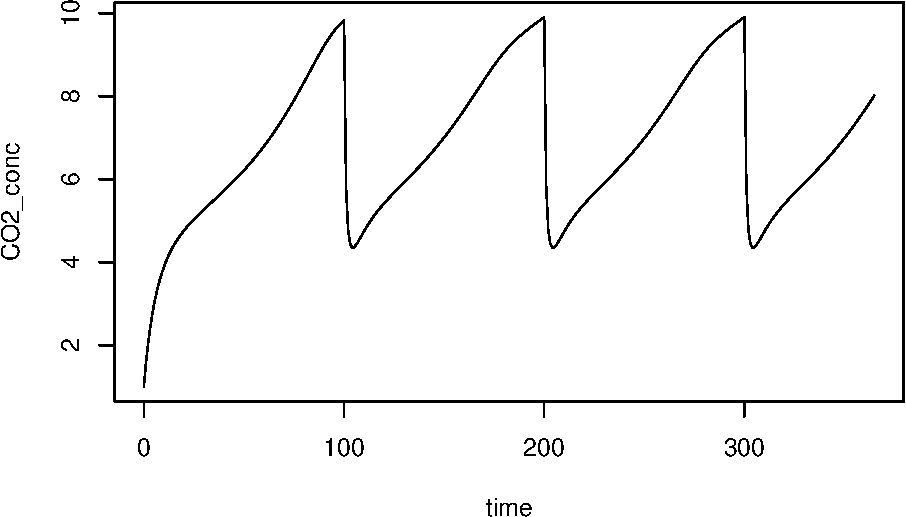
\includegraphics{simple_demo_files/figure-latex/unnamed-chunk-83-1.pdf}

\hypertarget{co2-emission}{%
\section{11. CO2 emission}\label{co2-emission}}

CO2 emission can be includes through the volatilization route. It can be
produced from both fermentation and methanogenesis. Speciation of
dissolved CO2 (really H2CO3*) and HCO3- needs to be included (although a
reduced mass transfer coefficient could achieve the same effect). So
far, CO2 emission behavior is troublesome--it is difficult to produce
plausible results.

\begin{Shaded}
\begin{Highlighting}[]
\NormalTok{sub\_pars11 }\OtherTok{\textless{}{-}} \FunctionTok{list}\NormalTok{(}\AttributeTok{subs =} \FunctionTok{c}\NormalTok{(}\StringTok{\textquotesingle{}VSd\textquotesingle{}}\NormalTok{),}
                   \AttributeTok{forms =} \FunctionTok{c}\NormalTok{(}\AttributeTok{VSd =} \StringTok{\textquotesingle{}C23H37O14N (CO2)1.5\textquotesingle{}}\NormalTok{),}
                   \AttributeTok{T\_opt\_hyd =} \FunctionTok{c}\NormalTok{(}\AttributeTok{all =} \DecValTok{60}\NormalTok{),}
                   \AttributeTok{T\_min\_hyd =} \FunctionTok{c}\NormalTok{(}\AttributeTok{all =} \DecValTok{0}\NormalTok{),}
                   \AttributeTok{T\_max\_hyd =} \FunctionTok{c}\NormalTok{(}\AttributeTok{all =} \DecValTok{90}\NormalTok{),}
                   \AttributeTok{hydrol\_opt =} \FunctionTok{c}\NormalTok{(}\AttributeTok{all =} \FloatTok{0.1}\NormalTok{),}
                   \AttributeTok{sub\_fresh =} \FunctionTok{c}\NormalTok{(}\AttributeTok{VSd =} \DecValTok{20}\NormalTok{),}
                   \AttributeTok{sub\_init =} \FunctionTok{c}\NormalTok{(}\AttributeTok{VSd =} \DecValTok{20}\NormalTok{))}
\end{Highlighting}
\end{Shaded}

\begin{Shaded}
\begin{Highlighting}[]
\NormalTok{man\_pars11 }\OtherTok{\textless{}{-}} \FunctionTok{list}\NormalTok{(}\AttributeTok{comps =} \FunctionTok{c}\NormalTok{(}\StringTok{\textquotesingle{}CO2\textquotesingle{}}\NormalTok{, }\StringTok{\textquotesingle{}NH4p\textquotesingle{}}\NormalTok{),}
                 \AttributeTok{comp\_fresh =} \FunctionTok{c}\NormalTok{(}\AttributeTok{CO2 =} \DecValTok{1}\NormalTok{, }\AttributeTok{NH4p =} \FloatTok{2.5}\NormalTok{), }
                 \AttributeTok{VFA\_fresh =} \FunctionTok{c}\NormalTok{(}\AttributeTok{CH3COOH =} \DecValTok{2}\NormalTok{),}
                 \AttributeTok{pH =} \DecValTok{7}\NormalTok{, }\AttributeTok{dens =} \DecValTok{1000}\NormalTok{)}
\end{Highlighting}
\end{Shaded}

Here we will define speciation only for TIC. There is no way to include
CO3-2 as a third species.

\begin{Shaded}
\begin{Highlighting}[]
\NormalTok{chem\_pars11 }\OtherTok{\textless{}{-}} \FunctionTok{list}\NormalTok{(}\AttributeTok{COD\_conv =} \FunctionTok{c}\NormalTok{(}\AttributeTok{CH4 =} \DecValTok{1}\SpecialCharTok{/}\FloatTok{0.2507}\NormalTok{),}
                     \AttributeTok{specs =} \FunctionTok{c}\NormalTok{(}\StringTok{\textquotesingle{}HCO3m\textquotesingle{}}\NormalTok{),}
                     \AttributeTok{mspec =} \FunctionTok{c}\NormalTok{(}\AttributeTok{HCO3m =} \StringTok{\textquotesingle{}CO2\textquotesingle{}}\NormalTok{, }\AttributeTok{NH3 =} \StringTok{\textquotesingle{}NH4p\textquotesingle{}}\NormalTok{),}
                     \AttributeTok{lka =} \FunctionTok{c}\NormalTok{(}\AttributeTok{HCO3m =} \StringTok{\textquotesingle{}{-}2.778 + {-}353.5305 {-}0.06092*temp\_K + 21834.37/temp\_K + 126.8339*log10(temp\_K) {-}1684915/temp\_K\^{}2\textquotesingle{}}\NormalTok{),}
                     \AttributeTok{stoich =} \StringTok{\textquotesingle{}calc\textquotesingle{}}\NormalTok{,}
                     \AttributeTok{kl =} \FunctionTok{c}\NormalTok{(}\AttributeTok{CO2 =} \FloatTok{0.01}\NormalTok{) }\SpecialCharTok{*} \DecValTok{86400}\NormalTok{)}
\end{Highlighting}
\end{Shaded}

\begin{Shaded}
\begin{Highlighting}[]
\NormalTok{devtools}\SpecialCharTok{::}\FunctionTok{load\_all}\NormalTok{()}
\end{Highlighting}
\end{Shaded}

\begin{verbatim}
## i Loading ABM
\end{verbatim}

\begin{Shaded}
\begin{Highlighting}[]
\NormalTok{out11 }\OtherTok{\textless{}{-}} \FunctionTok{abm}\NormalTok{(}\DecValTok{365}\NormalTok{,}
            \AttributeTok{mng\_pars =}\NormalTok{ mng\_pars,}
            \AttributeTok{man\_pars =}\NormalTok{ man\_pars11,}
            \AttributeTok{grp\_pars =}\NormalTok{ grp\_pars,}
            \AttributeTok{mic\_pars =}\NormalTok{ mic\_pars,}
            \AttributeTok{sub\_pars =}\NormalTok{ sub\_pars11,}
            \AttributeTok{chem\_pars =}\NormalTok{ chem\_pars11)}
\end{Highlighting}
\end{Shaded}

\begin{verbatim}
## Warning in expandPars(pars = pars, elnms = pars$grps, parnms = grp_par_nms):
## Size-variable parameter problem: Missing element(s) in kss.
\end{verbatim}

\begin{verbatim}
## Warning in checkCOD(dat = dat, grps = pars$grps, subs = pars$subs, COD_conv =
## pars$COD_conv, : COD balance is off by 1.8%
\end{verbatim}

TIC in slurry shows a lot of change over time, but can be kept away from
0 by adjusting kl. The low slurry level leads to a high relative loss.

\begin{Shaded}
\begin{Highlighting}[]
\FunctionTok{plot}\NormalTok{(CO2\_conc }\SpecialCharTok{\textasciitilde{}}\NormalTok{ time, }\AttributeTok{data =}\NormalTok{ out11, }\AttributeTok{type =} \StringTok{\textquotesingle{}l\textquotesingle{}}\NormalTok{, }\AttributeTok{ylim =} \FunctionTok{c}\NormalTok{(}\DecValTok{0}\NormalTok{, }\DecValTok{3}\NormalTok{))}
\end{Highlighting}
\end{Shaded}

\includegraphics{simple_demo_files/figure-latex/unnamed-chunk-88-1.pdf}

But now we can predict a CO2:CH4 ratio. This is a cumulative value.

\begin{Shaded}
\begin{Highlighting}[]
\FunctionTok{plot}\NormalTok{(CO2\_emis\_cum }\SpecialCharTok{/}\NormalTok{ CH4\_emis\_cum }\SpecialCharTok{\textasciitilde{}}\NormalTok{ time, }\AttributeTok{data =}\NormalTok{ out11, }\AttributeTok{type =} \StringTok{\textquotesingle{}l\textquotesingle{}}\NormalTok{, }\AttributeTok{ylab =} \StringTok{\textquotesingle{}CO2:CH4\textquotesingle{}}\NormalTok{)}
\end{Highlighting}
\end{Shaded}

\includegraphics{simple_demo_files/figure-latex/unnamed-chunk-89-1.pdf}

\begin{Shaded}
\begin{Highlighting}[]
\FunctionTok{plot}\NormalTok{(CO2\_emis\_cum }\SpecialCharTok{/}\NormalTok{ CH4\_emis\_cum }\SpecialCharTok{\textasciitilde{}}\NormalTok{ time, }\AttributeTok{data =}\NormalTok{ out11, }\AttributeTok{type =} \StringTok{\textquotesingle{}l\textquotesingle{}}\NormalTok{, }\AttributeTok{ylab =} \StringTok{\textquotesingle{}CO2:CH4\textquotesingle{}}\NormalTok{, }\AttributeTok{ylim =} \FunctionTok{c}\NormalTok{(}\DecValTok{0}\NormalTok{, }\DecValTok{5}\NormalTok{))}
\FunctionTok{abline}\NormalTok{(}\AttributeTok{h =} \DecValTok{1}\NormalTok{, }\AttributeTok{lty =} \DecValTok{2}\NormalTok{)}
\end{Highlighting}
\end{Shaded}

\includegraphics{simple_demo_files/figure-latex/unnamed-chunk-89-2.pdf}

Let's try some different substrates.

\hypertarget{respiration}{%
\section{12. Respiration}\label{respiration}}

To include respiration just add a \texttt{kl} value for \texttt{O2}.

\begin{Shaded}
\begin{Highlighting}[]
\NormalTok{chem\_pars12a }\OtherTok{\textless{}{-}} \FunctionTok{list}\NormalTok{(}\AttributeTok{COD\_conv =} \FunctionTok{c}\NormalTok{(}\AttributeTok{CH4 =} \DecValTok{1}\SpecialCharTok{/}\FloatTok{0.2507}\NormalTok{))}

\NormalTok{chem\_pars12b }\OtherTok{\textless{}{-}} \FunctionTok{list}\NormalTok{(}\AttributeTok{COD\_conv =} \FunctionTok{c}\NormalTok{(}\AttributeTok{CH4 =} \DecValTok{1}\SpecialCharTok{/}\FloatTok{0.2507}\NormalTok{),}
                     \AttributeTok{kl =} \FunctionTok{c}\NormalTok{(}\AttributeTok{O2 =} \FloatTok{0.1}\NormalTok{) }\SpecialCharTok{*} \DecValTok{86400}\NormalTok{)}
\end{Highlighting}
\end{Shaded}

\begin{Shaded}
\begin{Highlighting}[]
\NormalTok{devtools}\SpecialCharTok{::}\FunctionTok{load\_all}\NormalTok{()}
\end{Highlighting}
\end{Shaded}

\begin{verbatim}
## i Loading ABM
\end{verbatim}

\begin{Shaded}
\begin{Highlighting}[]
\NormalTok{out12a }\OtherTok{\textless{}{-}} \FunctionTok{abm}\NormalTok{(}\DecValTok{365}\NormalTok{,}
             \AttributeTok{mng\_pars =}\NormalTok{ mng\_pars,}
             \AttributeTok{man\_pars =}\NormalTok{ man\_pars,}
             \AttributeTok{grp\_pars =}\NormalTok{ grp\_pars,}
             \AttributeTok{mic\_pars =}\NormalTok{ mic\_pars,}
             \AttributeTok{sub\_pars =}\NormalTok{ sub\_pars,}
             \AttributeTok{chem\_pars =}\NormalTok{ chem\_pars12a,}
\NormalTok{)}
\end{Highlighting}
\end{Shaded}

\begin{verbatim}
## Warning in expandPars(pars = pars, elnms = pars$grps, parnms = grp_par_nms):
## Size-variable parameter problem: Missing element(s) in kss.
\end{verbatim}

\begin{verbatim}
## Warning in checkCOD(dat = dat, grps = pars$grps, subs = pars$subs, COD_conv =
## pars$COD_conv, : COD balance is off by 1.7%
\end{verbatim}

\begin{Shaded}
\begin{Highlighting}[]
\NormalTok{devtools}\SpecialCharTok{::}\FunctionTok{load\_all}\NormalTok{()}
\end{Highlighting}
\end{Shaded}

\begin{verbatim}
## i Loading ABM
\end{verbatim}

\begin{Shaded}
\begin{Highlighting}[]
\NormalTok{out12b }\OtherTok{\textless{}{-}} \FunctionTok{abm}\NormalTok{(}\DecValTok{365}\NormalTok{,}
             \AttributeTok{mng\_pars =}\NormalTok{ mng\_pars,}
             \AttributeTok{man\_pars =}\NormalTok{ man\_pars,}
             \AttributeTok{grp\_pars =}\NormalTok{ grp\_pars,}
             \AttributeTok{mic\_pars =}\NormalTok{ mic\_pars,}
             \AttributeTok{sub\_pars =}\NormalTok{ sub\_pars,}
             \AttributeTok{chem\_pars =}\NormalTok{ chem\_pars12b,}
\NormalTok{)}
\end{Highlighting}
\end{Shaded}

\begin{verbatim}
## Warning in expandPars(pars = pars, elnms = pars$grps, parnms = grp_par_nms):
## Size-variable parameter problem: Missing element(s) in kss.
\end{verbatim}

\begin{verbatim}
## Warning in checkCOD(dat = dat, grps = pars$grps, subs = pars$subs, COD_conv =
## pars$COD_conv, : COD balance is off by 3.3%
\end{verbatim}

\begin{Shaded}
\begin{Highlighting}[]
\FunctionTok{plot}\NormalTok{(CH4\_emis\_cum }\SpecialCharTok{\textasciitilde{}}\NormalTok{ time, }\AttributeTok{data =}\NormalTok{ out12a, }\AttributeTok{type =} \StringTok{\textquotesingle{}l\textquotesingle{}}\NormalTok{)}
\FunctionTok{lines}\NormalTok{(CH4\_emis\_cum }\SpecialCharTok{\textasciitilde{}}\NormalTok{ time, }\AttributeTok{data =}\NormalTok{ out12b, }\AttributeTok{col =} \StringTok{\textquotesingle{}red\textquotesingle{}}\NormalTok{)}
\end{Highlighting}
\end{Shaded}

\includegraphics{simple_demo_files/figure-latex/unnamed-chunk-93-1.pdf}

To track CO2 emission, we need all the inputs used in example 11.

\begin{Shaded}
\begin{Highlighting}[]
\NormalTok{man\_pars12 }\OtherTok{\textless{}{-}} \FunctionTok{list}\NormalTok{(}\AttributeTok{comps =} \FunctionTok{c}\NormalTok{(}\StringTok{\textquotesingle{}CO2\textquotesingle{}}\NormalTok{, }\StringTok{\textquotesingle{}NH4p\textquotesingle{}}\NormalTok{),}
                   \AttributeTok{comp\_fresh =} \FunctionTok{c}\NormalTok{(}\AttributeTok{CO2 =} \DecValTok{1}\NormalTok{, }\AttributeTok{NH4p =} \DecValTok{3}\NormalTok{), }
                   \AttributeTok{VFA\_fresh =} \FunctionTok{c}\NormalTok{(}\AttributeTok{CH3COOH =} \DecValTok{2}\NormalTok{),}
                   \AttributeTok{pH =} \DecValTok{7}\NormalTok{, }\AttributeTok{dens =} \DecValTok{1000}\NormalTok{)}
\end{Highlighting}
\end{Shaded}

\begin{Shaded}
\begin{Highlighting}[]
\NormalTok{chem\_pars12c }\OtherTok{\textless{}{-}} \FunctionTok{list}\NormalTok{(}\AttributeTok{COD\_conv =} \FunctionTok{c}\NormalTok{(}\AttributeTok{CH4 =} \DecValTok{1}\SpecialCharTok{/}\FloatTok{0.2507}\NormalTok{),}
                     \AttributeTok{specs =} \FunctionTok{c}\NormalTok{(}\StringTok{\textquotesingle{}HCO3m\textquotesingle{}}\NormalTok{),}
                     \AttributeTok{mspec =} \FunctionTok{c}\NormalTok{(}\AttributeTok{HCO3m =} \StringTok{\textquotesingle{}CO2\textquotesingle{}}\NormalTok{, }\AttributeTok{NH3 =} \StringTok{\textquotesingle{}NH4p\textquotesingle{}}\NormalTok{),}
                     \AttributeTok{lka =} \FunctionTok{c}\NormalTok{(}\AttributeTok{HCO3m =} \StringTok{\textquotesingle{}{-}2.778 + {-}353.5305 {-}0.06092*temp\_K + 21834.37/temp\_K + 126.8339*log10(temp\_K) {-}1684915/temp\_K\^{}2\textquotesingle{}}\NormalTok{),}
                     \AttributeTok{stoich =} \StringTok{\textquotesingle{}calc\textquotesingle{}}\NormalTok{,}
                     \AttributeTok{kl =} \FunctionTok{c}\NormalTok{(}\AttributeTok{CO2 =} \FloatTok{0.01}\NormalTok{) }\SpecialCharTok{*} \DecValTok{86400}\NormalTok{)}
\end{Highlighting}
\end{Shaded}

\begin{Shaded}
\begin{Highlighting}[]
\NormalTok{chem\_pars12d }\OtherTok{\textless{}{-}} \FunctionTok{list}\NormalTok{(}\AttributeTok{COD\_conv =} \FunctionTok{c}\NormalTok{(}\AttributeTok{CH4 =} \DecValTok{1}\SpecialCharTok{/}\FloatTok{0.2507}\NormalTok{),}
                     \AttributeTok{specs =} \FunctionTok{c}\NormalTok{(}\StringTok{\textquotesingle{}HCO3m\textquotesingle{}}\NormalTok{),}
                     \AttributeTok{mspec =} \FunctionTok{c}\NormalTok{(}\AttributeTok{HCO3m =} \StringTok{\textquotesingle{}CO2\textquotesingle{}}\NormalTok{, }\AttributeTok{NH3 =} \StringTok{\textquotesingle{}NH4p\textquotesingle{}}\NormalTok{),}
                     \AttributeTok{lka =} \FunctionTok{c}\NormalTok{(}\AttributeTok{HCO3m =} \StringTok{\textquotesingle{}{-}2.778 + {-}353.5305 {-}0.06092*temp\_K + 21834.37/temp\_K + 126.8339*log10(temp\_K) {-}1684915/temp\_K\^{}2\textquotesingle{}}\NormalTok{),}
                     \AttributeTok{stoich =} \StringTok{\textquotesingle{}calc\textquotesingle{}}\NormalTok{,}
                     \AttributeTok{kl =} \FunctionTok{c}\NormalTok{(}\AttributeTok{O2 =} \FloatTok{0.1}\NormalTok{, }\AttributeTok{CO2 =} \FloatTok{0.01}\NormalTok{) }\SpecialCharTok{*} \DecValTok{86400}\NormalTok{)}
\end{Highlighting}
\end{Shaded}

(Hmm, shouldn't \texttt{stoich} be part of \texttt{sub\_pars}?)

We also need stoichiometry for CO2, so we need a substrate chemical
formula.

\begin{Shaded}
\begin{Highlighting}[]
\NormalTok{sub\_pars12 }\OtherTok{\textless{}{-}} \FunctionTok{list}\NormalTok{(}\AttributeTok{subs =} \FunctionTok{c}\NormalTok{(}\StringTok{\textquotesingle{}VSd\textquotesingle{}}\NormalTok{),}
                   \AttributeTok{forms =} \FunctionTok{c}\NormalTok{(}\AttributeTok{VSd =} \StringTok{\textquotesingle{}C23H37O14N (CO2)1.5\textquotesingle{}}\NormalTok{),}
                   \AttributeTok{T\_opt\_hyd =} \FunctionTok{c}\NormalTok{(}\AttributeTok{all =} \DecValTok{60}\NormalTok{),}
                   \AttributeTok{T\_min\_hyd =} \FunctionTok{c}\NormalTok{(}\AttributeTok{all =} \DecValTok{0}\NormalTok{),}
                   \AttributeTok{T\_max\_hyd =} \FunctionTok{c}\NormalTok{(}\AttributeTok{all =} \DecValTok{90}\NormalTok{),}
                   \AttributeTok{hydrol\_opt =} \FunctionTok{c}\NormalTok{(}\AttributeTok{all =} \FloatTok{0.1}\NormalTok{),}
                   \AttributeTok{sub\_fresh =} \FunctionTok{c}\NormalTok{(}\AttributeTok{VSd =} \DecValTok{20}\NormalTok{),}
                   \AttributeTok{sub\_init =} \FunctionTok{c}\NormalTok{(}\AttributeTok{VSd =} \DecValTok{20}\NormalTok{))}
\end{Highlighting}
\end{Shaded}

\begin{Shaded}
\begin{Highlighting}[]
\NormalTok{devtools}\SpecialCharTok{::}\FunctionTok{load\_all}\NormalTok{()}
\end{Highlighting}
\end{Shaded}

\begin{verbatim}
## i Loading ABM
\end{verbatim}

\begin{Shaded}
\begin{Highlighting}[]
\NormalTok{out12c }\OtherTok{\textless{}{-}} \FunctionTok{abm}\NormalTok{(}\DecValTok{365}\NormalTok{,}
             \AttributeTok{mng\_pars =}\NormalTok{ mng\_pars,}
             \AttributeTok{man\_pars =}\NormalTok{ man\_pars12,}
             \AttributeTok{grp\_pars =}\NormalTok{ grp\_pars,}
             \AttributeTok{mic\_pars =}\NormalTok{ mic\_pars,}
             \AttributeTok{sub\_pars =}\NormalTok{ sub\_pars12,}
             \AttributeTok{chem\_pars =}\NormalTok{ chem\_pars12c,}
\NormalTok{)}
\end{Highlighting}
\end{Shaded}

\begin{verbatim}
## Warning in expandPars(pars = pars, elnms = pars$grps, parnms = grp_par_nms):
## Size-variable parameter problem: Missing element(s) in kss.
\end{verbatim}

\begin{verbatim}
## Warning in checkCOD(dat = dat, grps = pars$grps, subs = pars$subs, COD_conv =
## pars$COD_conv, : COD balance is off by 1.8%
\end{verbatim}

\begin{Shaded}
\begin{Highlighting}[]
\NormalTok{devtools}\SpecialCharTok{::}\FunctionTok{load\_all}\NormalTok{()}
\end{Highlighting}
\end{Shaded}

\begin{verbatim}
## i Loading ABM
\end{verbatim}

\begin{Shaded}
\begin{Highlighting}[]
\NormalTok{out12d }\OtherTok{\textless{}{-}} \FunctionTok{abm}\NormalTok{(}\DecValTok{365}\NormalTok{,}
             \AttributeTok{mng\_pars =}\NormalTok{ mng\_pars,}
             \AttributeTok{man\_pars =}\NormalTok{ man\_pars12,}
             \AttributeTok{grp\_pars =}\NormalTok{ grp\_pars,}
             \AttributeTok{mic\_pars =}\NormalTok{ mic\_pars,}
             \AttributeTok{sub\_pars =}\NormalTok{ sub\_pars12,}
             \AttributeTok{chem\_pars =}\NormalTok{ chem\_pars12d,}
\NormalTok{)}
\end{Highlighting}
\end{Shaded}

\begin{verbatim}
## Warning in expandPars(pars = pars, elnms = pars$grps, parnms = grp_par_nms):
## Size-variable parameter problem: Missing element(s) in kss.
\end{verbatim}

\begin{verbatim}
## Warning in checkCOD(dat = dat, grps = pars$grps, subs = pars$subs, COD_conv =
## pars$COD_conv, : COD balance is off by 5.6%
\end{verbatim}

See how COD balance is worse?

\begin{Shaded}
\begin{Highlighting}[]
\FunctionTok{plot}\NormalTok{(CH4\_emis\_cum }\SpecialCharTok{\textasciitilde{}}\NormalTok{ time, }\AttributeTok{data =}\NormalTok{ out12c, }\AttributeTok{type =} \StringTok{\textquotesingle{}l\textquotesingle{}}\NormalTok{)}
\FunctionTok{lines}\NormalTok{(CH4\_emis\_cum }\SpecialCharTok{\textasciitilde{}}\NormalTok{ time, }\AttributeTok{data =}\NormalTok{ out12d, }\AttributeTok{col =} \StringTok{\textquotesingle{}red\textquotesingle{}}\NormalTok{)}
\end{Highlighting}
\end{Shaded}

\includegraphics{simple_demo_files/figure-latex/unnamed-chunk-100-1.pdf}

\begin{Shaded}
\begin{Highlighting}[]
\FunctionTok{plot}\NormalTok{(CO2\_emis\_cum }\SpecialCharTok{\textasciitilde{}}\NormalTok{ time, }\AttributeTok{data =}\NormalTok{ out12c, }\AttributeTok{type =} \StringTok{\textquotesingle{}l\textquotesingle{}}\NormalTok{)}
\FunctionTok{lines}\NormalTok{(CO2\_emis\_cum }\SpecialCharTok{\textasciitilde{}}\NormalTok{ time, }\AttributeTok{data =}\NormalTok{ out12d, }\AttributeTok{col =} \StringTok{\textquotesingle{}red\textquotesingle{}}\NormalTok{)}
\end{Highlighting}
\end{Shaded}

\includegraphics{simple_demo_files/figure-latex/unnamed-chunk-101-1.pdf}

\end{document}
